\documentclass[11pt,a4paper]{article}
\usepackage[T1]{fontenc}
\usepackage{amsmath,amssymb,amsthm,mathtools}
\usepackage[margin=26mm]{geometry}
\usepackage{lmodern,microtype,booktabs,graphicx,array,longtable}
\usepackage[hidelinks]{hyperref}\usepackage{xurl}
\hypersetup{pdftitle={OEIS A290268 at Unbounded Logarithmic Deficit},pdfauthor={ProveIt research report (AI-assisted), built from research notes prepared for Vladimir Reshetnikov with OpenAI}}
\setlength{\parskip}{3pt}
\setlength{\emergencystretch}{2em}
\setlength{\LTcapwidth}{\textwidth}
\numberwithin{equation}{section}
\newtheorem{theorem}{Theorem}[section]
\newtheorem{lemma}[theorem]{Lemma}
\newtheorem{proposition}[theorem]{Proposition}
\newtheorem{corollary}[theorem]{Corollary}
\newtheorem{question}{Question}
\newcommand{\fall}[2]{(#1)_{\underline{#2}}}
\newcommand{\Ai}{\operatorname{Ai}}
\newcommand{\mergenote}[1]{\par\smallskip\noindent{\small\textsf{[Merge note, batch 72A.]} #1}\par\smallskip}
\newcommand{\addednote}[1]{{\small[\textit{Added 1 October 2026, batch 72A:} #1]}}
\title{OEIS A290268 at Unbounded Logarithmic Deficit\\[6pt]
\large Regular saddle phases, the Airy fold, two-dimensional cosine laws,\\
superseded lower bounds, and arithmetic families}
\author{ProveIt research report, built from eight research notes\\
prepared for Vladimir Reshetnikov with OpenAI (batch~72A)}
\date{1 October 2026}
\begin{document}\maketitle
\begin{abstract}
OEIS A290268 counts the nonzero terms $a(N)$ in the $N$th derivative of $x^{x^2}$. In the depth coordinates of the source report, each term is an integer $H_{d,k,q}$, and the depth $d$ is the logarithmic deficit. This report collects eight manuscripts on the regime in which that deficit grows with the derivative order, merged into four parts. Part~I determines a regular saddle branch $\kappa=\sin t/t-2\cos t-2$, $t_0\le t<t_c$, ending at a curvature-zero fold $\kappa_c\approx0.0281461$. On it, a uniform fixed-offset phase law proves eventual nonvanishing at every algebraic limiting ratio $k/d\to\kappa<\kappa_c$, and uniformly for $|b|\le8$ and $0\le k\le d/36$. Possible phase zeros lie only on explicit transcendental rays. An $O(1/d)$ rate confines possible extra zeros near those rays to bounded strips, and the phase law persists for offsets $|b|\le\sqrt d$. The fixed-logarithmic-degree phase laws of the arithmetic manuscript are the case $\kappa=0$. Part~II proves an additive Airy law in the critical window $|k-\kappa_cd|=O(d^{1/3})$, and hence eventual nonvanishing at the nearest integer to $\kappa_cd$. Part~III proves uniform two-dimensional cosine laws, explicit phase curvatures, density one with $O(N^{5/3})$ exceptions on tail patches, and uniform positivity on the triangle $40k+420q\le91d$. It also records the lower bounds these gave: $a(N)\ge(3/8+c)N^2$, $a(N)\ge3N^2/8+CN^{3/2}$, and $\liminf a(N)/N^2\ge28176/57247$. All of them are ineffective, and all are superseded by $a(N)=N^2/2+o(N^2)$, proved in the sibling report \emph{power-tower-exponent-supports}. Part~IV proves block congruences modulo primes, prime-unit families with exact valuations at unbounded depth, all-depth central strips at $k=0$, and an exact example showing that root geometry alone cannot prove the support conjecture. The full support conjecture remains open, no numerical depth threshold is asserted, and nothing here is formally verified.
\end{abstract}
\tableofcontents
\clearpage

\section{Introduction}\label{aud:sec:intro}
Write
\[
 \frac{d^N}{dx^N}x^{x^2}
 =x^{x^2}\sum_{j\in\mathbb Z,\,k\ge0}c_N(j,k)x^j(\log x)^k,
\]
and let $a(N)$ be the number of pairs $(j,k)$ with $c_N(j,k)\ne0$; this is OEIS A290268. The ProveIt research report \emph{power-tower-derivative-term-counts}, cited here as~\cite{source}, studies this count in its Part~3. Its Section~3.15 reduces every coefficient with $j\le-1$ to an integer $H_{d,k,q}$ in \emph{depth coordinates} (Section~\ref{aud:sec:model} below). It proves that the reflection holes $q=2d$, $k+d$ even, vanish, classifies depths one through four completely, and conjectures that there are no other zeros. That conjecture is its complete support classification, label \texttt{xxb:conj:support}. Its Questions~4 and~5 (Section~3.24) ask for results uniform in the depth and for arithmetic separation of real zeros.

The manuscripts collected here study the coefficients when the depth $d$ grows with $N$. In the manuscripts' words, this is the regime of \emph{unbounded logarithmic deficit}: the depth is the deficit $m=k-j$ of the source's Part~3 proper. Every manuscript was written against the source at commit \texttt{ca81647a9}.

\subsection{How the report is organized}\label{aud:sec:organization}
\begin{itemize}
\item \textbf{Part~\ref{aud:part:I}}, the regular saddle branch and fixed-offset phases: manuscript~58 (the base of the merge, Sections~\ref{aud:sec:model}--\ref{aud:sec:58scope}); manuscript~64's fixed-degree phase laws as the case $\kappa=0$ (Sections~\ref{aud:sec:kappa0}--\ref{aud:sec:kappa0k}); manuscript~45's absolute rate and bounded strips (Section~\ref{aud:sec:45a}); and manuscript~53's phase law through square-root offsets (Section~\ref{aud:sec:53a}).
\item \textbf{Part~\ref{aud:part:II}}, the Airy fold at $\kappa_c$: manuscript~54.
\item \textbf{Part~\ref{aud:part:III}}, the two-dimensional tail and the lower bounds: manuscripts~49, 45 (its second part), 40, 37 and the count of~53, followed by the table of superseded headline bounds (Section~\ref{aud:sec:headlines}).
\item \textbf{Part~\ref{aud:part:IV}}, arithmetic at unbounded deficit: manuscript~64's congruences, valuations, central strips and root-geometry example.
\item Questions (Section~\ref{aud:sec:questions}) and provenance (Section~\ref{aud:sec:provenance}).
\end{itemize}
Manuscript numbers are those of batch~72A (Section~\ref{aud:sec:provenance}). A ninth manuscript, 61, is wholly implied by~58 and is not printed; Section~\ref{aud:sec:provenance} says what it contained.

\subsection{What the merge printed once}\label{aud:sec:printedonce}
The members overlap heavily, and Vladimir asked for duplicates to be watched for. Each item below is printed once, credited to every manuscript that proved it, and the other copies are replaced by references.
\begin{itemize}
\item The coefficient model, derivative bridge and bulk count, restated by all eight manuscripts: Section~\ref{aud:sec:model}.
\item The regular-branch geometry (the functions $K,F,D_0$, the gap identity and the limiting curvature), proved in~58 and restated in~49, 53, 54 and~40: Proposition~\ref{aud:fr:branch}.
\item The exact-rational certificate $\kappa_c>1/36$, delivered byte for byte by~49, 53 and~58: Lemma~\ref{aud:fr:rationalband}. One copy of the script and its record is shipped.
\item The closed-walk trace estimate: in full as Lemma~\ref{aud:af:trace} (manuscript~54) and in its offset-dependent form as Lemma~\ref{aud:go:trace} (manuscript~53). Manuscripts~45 and~49 use it with a sketch, kept as citations.
\item The integer-triangle (Jarn\'ik-type) lemma, proved in~45 and repeated in~40 and~37: Lemma~\ref{aud:sc:lattice}.
\item The single-contour representation, derived in both~40 and~37: equation~\eqref{aud:dc:actionintegral}.
\item The two-saddle cosine law of~49, which~45 restates as its input: Theorem~\ref{aud:qg:cosine}.
\item The fixed-degree phase laws of~64 are the case $\kappa=0$ of~58's phase theorem. They are printed as corollaries, with 64's proofs kept as second proofs (Section~\ref{aud:sec:kappa0}).
\end{itemize}
The headline count bounds of~37, 49, 53, 45 and~40 are all implied by the leading asymptotic $a(N)=N^2/2+o(N^2)$ of manuscript~34. That theorem is printed in the sibling report \emph{power-tower-exponent-supports}~\cite{pte}, not here. The bounds are kept, each with a dated note, because the cosine laws, phase structure, positivity and explicit constants behind them are not consequences of a count asymptotic. Section~\ref{aud:sec:headlines} states the relation exactly.

\subsection{Status}\label{aud:sec:status}
This is an AI-assisted research report. It is unrefereed and not formalized. Each manuscript's statement that its proofs ``received independent mathematical review'' is the authors' statement, kept as delivered; the intake checked selected constants and identities and reran the shipped scripts on copies (Section~\ref{aud:sec:provenance}). It did not re-derive every proof. No statement here has a Lean or Rocq counterpart. The A290268 Lean development at \nolinkurl{Combinatorics/DerivativeExpansions/A290268/Lean} formalizes the coefficient recurrence, the support window, the count of the conjectured support, the values $a(n)$ for $n\le53$, and the reduction of the conjectured closed form to a support statement (conditional). It contains none of the theorems of this report. Placement beside the source report confers no formal status. All thresholds in this report are existential unless a number is displayed.

Text added in the merge is marked \textsf{[Merge note, batch 72A.]} or \textit{[Added 1 October 2026, batch 72A: \dots]}. Everything else is the manuscripts' text, with the label prefixes, symbol renames and cross-references listed below.

\subsection{Conventions and notation}\label{aud:sec:conventions}
All parts use the depth coordinates of~\cite[Section 3.15]{source}: depth $d$, logarithmic degree $k$, tail index $q$, and the \emph{signed} offset $b=q-2d$. The following table fixes the remaining letters. It lists, for each, the tempting false reading from the source report or from another part. A letter marked ``local'' is defined where it is used and means nothing outside that section.

{\small
\begin{longtable}{@{}>{\raggedright\arraybackslash}p{0.17\textwidth}
 >{\raggedright\arraybackslash}p{0.36\textwidth}
 >{\raggedright\arraybackslash}p{0.39\textwidth}@{}}
\caption{Symbols of this report and their false readings.}\label{aud:tab:notation}\\
\toprule
Symbol & Meaning here & Not to be confused with\\
\midrule\endfirsthead
\toprule
Symbol & Meaning here & Not to be confused with\\
\midrule\endhead
$d,k,q$ & depth, power of $\log x$, tail index; $N=2k+2d+1+q$ & the source's Part~3 proper, where $d=n-2k-1$ and the depth is $m=k-j$\\
$b$ & signed offset $q-2d$ (Parts~I--III, and Part~IV except one section) & manuscript~64's $b=|2d-q|$ in its central-strip section; that quantity is written $s$ here (Section~\ref{aud:sec:k0strips})\\
$s,\sigma,\varepsilon,h$ & $s=|b|$, $\sigma=\pm1$, parity $\varepsilon=(d-k-1)\bmod 2$, $h=(d-k-1-\varepsilon)/2$ & the block residue $s$ of Theorem~\ref{aud:ap:thm:blocks}; the source's $h_d(\tau)$\\
$\kappa,\delta,\eta$ & ratios $k/d$, $b/d$, and $q/d=\delta+2$ (37, 40) & the source's $\delta=q-p$; manuscript~53's small constant, written $\eta_*$\\
$r$ & $2d+q+1=M-k$ (Section~\ref{aud:sec:model}, Parts~I, II, IV); in Part~III (37, 40, 45) the centered ratio parameter $4+\delta$ & the source's $r$ in $n=2r$, $n=2r+1$\\
$R$ & $4d+b+1$, equal to $2d+q+1$ when $q=2d+b$; $(4+\delta)d+1$ & ---\\
$M$ & coefficient index $k+r=N-k$ & the limiting mean, written $\mathcal M$; the source's moduli $M_1,M_2$\\
$\mathcal M(\kappa,y)$ & limiting saddle mean~\eqref{aud:fr:meanlimit} & renamed from $M$ in 58, 49, 53 and 54\\
$m$ & $\min(2d,q)$ & the source's deficit $m=k-j$\\
$\omega$ & dummy variable of the coefficient extraction $[\omega^M]$ & the source and the manuscripts write $w$; renamed because $w$ is the saddle radius\\
$w(\kappa),a(\kappa)$ & $w=1/t(\kappa)=\sqrt{y(\kappa)}$, $a=w/2$, equation~\eqref{aud:eq:wa}; $a_0=a(0)$ & the count $a(N)$; manuscript~64's $a$ is $a_0$\\
$t$, $T$ & branch parameter $t\in[t_0,t_c)$; written $T$ in 37 and 40, where $t$ is the contour variable ($T_0=t_0$, $T_c=t_c$) & in 45 and 54, local $T$ and $T_*$ are third logarithmic derivatives\\
$K,F,D_0$ & branch functions~\eqref{aud:fr:K}, \eqref{aud:fr:FD} & the source's cutoff constants $K_d$, falling factorial $F_n$ and Mellin transform $\mathcal F_{d,k}$\\
$D(v)=A(v)B(v)$ & Laurent product~\eqref{aud:fr:Laurent}; 49's $D_R$ & the source's $D_\delta$; 40's angular deficit, written $\Delta_{\rm ang}$\\
$\rho$ & finite-depth saddle radius, $\rho\approx d^2y$ & the source's count index $\rho$ in $\beta(2\rho)$\\
$\zeta$ & outer variable $u=d\zeta$ (49, Part~III) & the source's $\Pi_d(\zeta)$; 45's phase-crossing ratios, written $\kappa^\star$\\
$\mathcal P$ & analytic prefactor (49, 45); $P$ (40), $P_h$ (37); $P_d(u)=\fall{2d+u}{4d+b+1}$ & the source's falling product $\mathcal P_M$; 45's patch, written $\mathcal C_N$\\
$L$ & action $L(t)$ (37, 40); monic Jacobi polynomials $L_j$ (58); Airy constants $L_\varepsilon(b)$ (54); local $L^2=w^2+r^2/4$ (45) & the source's $L=\log x$\\
$U_b,Q_b$ & unpaired product and shift quotient (49, 53) & the source's $U(n)$; 37's kernel, written $\mathcal U(s,y)$\\
$G_k(c,r)$ & centered recurrence~\eqref{aud:fr:G}; 64 also writes $Q_k^{(R)}(u-b/2)$ and $C_j(c;R)$ & $G_k(c,r)=\mathcal Q_k^{(r)}(c/2)$ in the source's Part~3 notation\\
$\mathcal J$, $J_{d,k}$ & integral~\eqref{aud:fr:J}; Jacobi matrix & the source's zero budget $J(d,k)$\\
$E$ & $E(\kappa,y)=2\mathcal M+\kappa-1$ (58, 54); local elsewhere; $E_{m,r}$ elementary symmetric (64) & the source's $\mathsf E_q$; 53's error, written $\mathrm{Err}_{d,k,b}$\\
$\beta(N)$, $\beta_b$ & bulk count~\eqref{aud:bulk}; $\beta_b=|b|+1$ (53) & ---\\
$p$ & path length (trace lemmas); odd prime (Part~IV); integer in the exceptional ratios (58, 45) & local in each\\
$z$ & inner generating variable (49); local in 37 and 40 & the source's $z=x^2$\\
\bottomrule
\end{longtable}}

\paragraph{Renamed symbols.}
No normalization was changed. The renames are: the extraction variable $w\mapsto\omega$ (all manuscripts); the limiting mean $M(\kappa,y)\mapsto\mathcal M(\kappa,y)$ (58, 49, 53, 54); 54's Airy scale $c\mapsto c_A$; 45's phase-crossing ratios $\zeta\mapsto\kappa^\star$, its patch $\mathcal P_N\mapsto\mathcal C_N$, its lattice-lemma curvature constants $m,M\mapsto\gamma_-,\gamma_+$ and its lattice determinant $D\mapsto\Delta_3$; 49's chain lengths $M,M_d\mapsto n,n_d$, its harmonic remainder $\mathcal R(v,w)\mapsto\mathcal R_{\rm h}(v,w)$ and its rotated exponent $E(Z)\mapsto E_{\rm in}(Z)$; 53's small constant $\eta\mapsto\eta_*$, its depth threshold $D\mapsto d_*$ and its error $E_{d,k,b}\mapsto\mathrm{Err}_{d,k,b}$; 40's angular deficit $D(T,\kappa)\mapsto\Delta_{\rm ang}(T,\kappa)$; 37's kernel $U(s,y)\mapsto\mathcal U(s,y)$, its regions $U_\pm\mapsto\mathcal W_\pm$, its local $D=s^2+y^2\mapsto\Sigma$, $B(s)\mapsto B_h(s)$, $A(s)\mapsto A_h(s)$, $U(z),B(z),R(z),h(z)\mapsto S_A(z),S_B(z),\varrho(z),h_B(z)$ and $E=\mathrm e^3\mapsto E_3$; 64's recurrence variable $a\mapsto c$ in Part~IV, its auxiliary polynomial $F(z)\mapsto Y_p(z)$, its example polynomials $F,Q\mapsto F_\sharp,Q_\sharp$, its evaluation parameter $h\mapsto h'$, and, in its central-strip section, $b=|2d-q|\mapsto s$ with the summation index $s\mapsto\ell$.

Every label carries the prefix \texttt{aud:}. Labels from a manuscript carry its own prefix as a sub-prefix: \texttt{aud:fr:} (58), \texttt{aud:af:} (54), \texttt{aud:sc:} (45), \texttt{aud:qg:} (49), \texttt{aud:go:} (53), \texttt{aud:gh:} (37), \texttt{aud:dc:} (40, distinct from the source's \texttt{xxb:dc:}) and \texttt{aud:ap:} (64).

\section{The coefficient model and the explicit region}\label{aud:sec:model}
For integers $d\ge1$ and $k,q\ge0$, put $r=2d+q+1$ and $M=k+r$. The integer model from~\cite[Section 3.15]{source} is
\begin{equation}\label{aud:fr:H}
 H_{d,k,q}=\frac{M!}{d!}[\omega^M](2+\omega)^k(1+\omega)^{2d}\log^d(1+\omega).
\end{equation}
Define
\begin{equation}\label{aud:fr:G}
 G_0(c,r)=1,\quad G_1(c,r)=c,\qquad
 G_{j+1}(c,r)=cG_j(c,r)+j(j+r)G_{j-1}(c,r).
\end{equation}
The source's centered factorization is
\begin{equation}\label{aud:fr:factor}
 H_{d,k,q}=[u^d]\fall{2d+u}{r}\,G_k(2u+2d-q,r).
\end{equation}
These are the centered Meixner--Pollaczek polynomials $Q_j^{(r)}(c/2)$; the classical generating-function normalization is recorded in~\cite{dlmf}. The source proves the reflection zeros $q=2d$, $k+d$ even. Its full conjecture asserts that no other zeros occur.

In the derivative expansion of $x^{x^2}$, with coefficient $c_N(j,k)$ of $x^j(\log x)^k$ after division by $x^{x^2}$, the exact bridge is
\begin{equation}\label{aud:bridge}
 N=2k+2d+1+q,\qquad j=-q-1,\qquad
 c_N(j,k)=\binom Nk H_{d,k,q}.
\end{equation}
Consequently every nonvanishing result below proves the presence of its corresponding derivative term.
The source~\cite[Section 3.23]{source} proves the positive-bulk count
\begin{equation}\label{aud:bulk}
 \beta(N)=\begin{cases}
 (3N^2+10N+8)/8,&N\text{ even},\\
 (3N^2+12N+1)/8,&N\text{ odd}.
 \end{cases}
\end{equation}
This bulk consists of the nonnegative $x$-power columns and the positive $j=-1$ boundary. Cells with $q\ge1$, equivalently $j\le-2$, therefore add terms outside it. At fixed $N$, distinct pairs $(d,k)$ give distinct monomials $(j,k)$.

\mergenote{The model~\eqref{aud:fr:H}, the recurrence~\eqref{aud:fr:G}, the factorization~\eqref{aud:fr:factor}, the bridge~\eqref{aud:bridge} and the bulk count~\eqref{aud:bulk} are restated in every member manuscript (37, 40, 45, 49, 53, 54, 64); they are printed once, here. In the source they are Section~3.15 (the factorization is its Proposition \texttt{xxb:dc:prop:factor}), Theorem \texttt{xxb:dc:thm:holes} (the reflection holes) and Section~3.23 (the bulk, first proved as Theorem \texttt{xxb:thm:main-bounds}). The polynomials $G_k(c,r)$ are the source's $\mathcal Q_k^{(r)}(c/2)$.}


Fix an integer $b$ and set
\begin{gather*}
 q=2d+b,\quad R=4d+b+1,\quad m=\min(2d,q),\quad s=|b|,\quad
 P_d(u)=\fall{2d+u}{4d+b+1},\\
 \sigma=\begin{cases}1,&b\le0,\\-1,&b>0,\end{cases}
 \qquad \varepsilon=(d-k-1)\bmod2,\qquad
 h=\frac{d-k-1-\varepsilon}{2}.
\end{gather*}
All statements concern sufficiently large $d$, so that $q\ge0$.

The explicit region uses
\begin{equation}\label{aud:fr:Kintro}
 K(t)=\frac{\sin t}{t}-2\cos t-2,
 \qquad F(t)=(2t^2-1)\sin t+t\cos t.
\end{equation}
Let $t_0$ be the nonzero solution of $\tan(t_0/2)=2t_0$ in $(0,\pi)$, and let $t_c$ be the unique zero of $F$ in $(t_0,\pi)$. We prove below that $K$ increases strictly from zero to
\[
 \kappa_c=K(t_c),\qquad
 t_0\le t<t_c.
\]
Thus each $0\le\kappa<\kappa_c$ has a unique inverse $t=t(\kappa)$ on this branch. Put
\begin{equation}\label{aud:fr:phaseintro}
 y(\kappa)=t(\kappa)^{-2},\qquad
 \psi(\kappa)=\frac{\pi-t(\kappa)}2.
\end{equation}
We also write
\begin{equation}\label{aud:eq:wa}
 w(\kappa)=\frac1{t(\kappa)}=\sqrt{y(\kappa)},\qquad a(\kappa)=\frac{w(\kappa)}2,\qquad a_0=a(0)=\frac1{2t_0}.
\end{equation}
Manuscripts~45 and~49 use $w$, and~58 and~53 use $a$. The constant $a_0$ is manuscript~64's $a$ (Section~\ref{aud:sec:kappa0}).

For orientation only, $\kappa_c\approx0.0281461097171$.

\begin{theorem}[An explicit finite-ratio region]\label{aud:fr:main}
The following conclusions hold.
\begin{enumerate}
\item If $k/d\to\kappa$ for an algebraic real number $0\le\kappa<\kappa_c$, then for every fixed integer $b$, $H_{d,k,2d+b}$ is nonzero for all sufficiently large $d$, except for the exact reflection holes $b=0$, $k+d$ even.
\item If $I\subset[0,\kappa_c)$ is compact, then for all sufficiently large $d$, the same nonvanishing holds simultaneously for every integer $k$ with $k/d\in I$ and every integer $|b|\le8$. In particular, this holds throughout $0\le k\le d/36$.
\item For any other fixed $b$, a uniform parity-dependent phase law holds on every such compact interval. Its possible vanishing phases occur only at the explicit ratios
\[
 \kappa=K\bigl((1-p/s)\pi\bigr),\qquad s=|b|>0,
\]
whose arguments lie in $[t_0,t_c)$, with $p$ odd for $\varepsilon=0$ and $p$ even for $\varepsilon=1$. These ratios are transcendental. The phase law alone makes no claim of exact cancellation on those rays.
\end{enumerate}
\end{theorem}

No explicit depth threshold is asserted. The offset $b$ is fixed, and the curvature-zero endpoint $\kappa_c$ is excluded. The proof gives the full phase and its positive amplitude, not merely the stated nonvanishing corollaries.
\part{The regular saddle branch and fixed-offset phases}\label{aud:part:I}
Sections~\ref{aud:sec:model}--\ref{aud:sec:58scope} are manuscript~58, the base of this report. The three sections after them refine its phase law along fixed-offset lines. Section~\ref{aud:sec:kappa0} gives the case $\kappa=0$ with manuscript~64's proofs. Section~\ref{aud:sec:45a} gives manuscript~45's absolute $O(1/d)$ rate, and Section~\ref{aud:sec:53a} manuscript~53's extension to offsets $|b|\le\sqrt d$.

\section{The limiting Jacobi roots}
For each fixed $d$, the monic polynomials
\[
 L_j(x)=i^{-j}G_j(ix,R)
\]
obey
\[
 L_{j+1}(x)=xL_j(x)-j(j+R)L_{j-1}(x).
\]
Thus $L_k$ is the characteristic polynomial of the $k\times k$ real symmetric Jacobi matrix $J_{d,k}$ with zero diagonal and off-diagonal entries $\sqrt{j(j+R)}$, $1\le j<k$. Its roots $\lambda$ are real, simple, and symmetric. For every positive root put $\alpha=\lambda^2/4$. Then
\begin{equation}\label{aud:fr:rootproduct}
 G_k(2u,R)=(2u)^k\prod_{\lambda>0}(1+\alpha/u^2).
\end{equation}
Empty products are one, and empty root maxima are zero. The elementary matrix norm bound gives, for $k\ge2$,
\begin{equation}\label{aud:fr:rootbound}
 \max\alpha\le(k-1)(k-1+R).
\end{equation}

\begin{lemma}[A finite-mass arcsine mixture]\label{aud:fr:measurelemma}
If $k/d\to\kappa\ge0$, then the finite measures
\[
 \nu_{d,k}=\frac1d\sum_{L_k(\lambda)=0}\delta_{\lambda/d}
\]
converge weakly to the measure characterized by
\begin{equation}\label{aud:fr:measure}
 \int f\,d\nu_\kappa
 =\frac1\pi\int_0^\kappa\int_0^\pi
 f\bigl(2\sqrt{x(x+4)}\cos\theta\bigr)\,d\theta\,dx.
\end{equation}
The measure has total mass $\kappa$. For each continuous $f$ on a common compact spectral interval, convergence to the right-hand side with $\kappa=k/d$ is uniform when $k/d$ ranges over a compact interval.
\end{lemma}
\begin{proof}
The norm bound gives a common compact spectral interval whenever $k/d$ is bounded. Odd trace moments vanish. For a fixed even power $2p$, expand the diagonal entries of $(J_{d,k}/d)^{2p}$ as sums over nearest-neighbor returning paths. Away from the $O(p)$ boundary rows, there are $\binom{2p}{p}$ such paths. At a row with $j/d\to x$, every path product tends to $[x(x+4)]^p$. The convergence is uniform on compact $x$ intervals, because $\sqrt{x(x+4)}$ is continuous there. The boundary rows contribute $o(1)$ after dividing the trace by $d$. Riemann sums therefore give
\[
 \frac1d\operatorname{tr}(J_{d,k}/d)^{2p}
 \longrightarrow\binom{2p}{p}\int_0^\kappa[x(x+4)]^p\,dx.
\]
These are exactly the moments of~\eqref{aud:fr:measure}; the zeroth moment is $k/d\to\kappa$. Polynomial approximation on the common compact support proves weak convergence. The case $\kappa=0$ also follows directly from the vanishing total mass. Uniformity follows by the same estimates, or by extracting a convergent subsequence from any hypothetical sequence violating it.
\end{proof}

Lemma~\ref{aud:fr:measurelemma} is an elementary specialization of the classical varying-recurrence zero-distribution theorem of Kuijlaars and Van Assche~\cite[Theorem 1.4]{kuijlaars}. The proof above is included so that no general zero-distribution theorem is required for the argument.

\section{The exterior saddle and its regular branch}
Define
\begin{equation}\label{aud:fr:Laurent}
 D(v)=A(v)B(v),\qquad
 A(v)=\prod_{j=1}^m(1+v/j^2),\qquad
 B(v)=\prod_{\lambda>0}(1-\alpha/v).
\end{equation}
For $\rho>\max\alpha$, the value $D(\rho)$ is positive, and
\begin{align}
 \mu(\rho)&=\frac{\rho D'(\rho)}{D(\rho)}
 =\sum_{j=1}^m\frac{\rho}{\rho+j^2}
   +\sum_{\lambda>0}\frac{\alpha}{\rho-\alpha},
 \label{aud:fr:mean}\\
 V(\rho)&=\frac{d\mu}{d\log\rho}=V_A-V_B,
 \label{aud:fr:curvaturefinite}\\
 V_A&=\sum_{j=1}^m\frac{\rho j^2}{(\rho+j^2)^2},\qquad
 V_B=\sum_{\lambda>0}\frac{\alpha\rho}{(\rho-\alpha)^2}.
 \nonumber
\end{align}
Write $\rho=d^2y$. If $k/d\to\kappa$ and $y>\kappa(\kappa+4)$, the norm bound separates this radius from all roots. Lemma~\ref{aud:fr:measurelemma} gives
\begin{equation}\label{aud:fr:meanlimit}
 \frac{\mu(d^2y)}d\longrightarrow \mathcal M(\kappa,y)
 =\sqrt y\arctan\frac2{\sqrt y}
 +\frac12\int_0^\kappa
 \left(\sqrt{\frac y{y-x(x+4)}}-1\right)\,dx.
\end{equation}
The factor $1/2$ counts one root from each symmetric pair; a possible zero root contributes zero. The convergence, including derivatives in $y$, is uniform on compact subsets of the strict exterior region. Indeed all the rational test functions and their derivatives are uniformly bounded there.

Put
\begin{equation}\label{aud:fr:J}
 \mathcal J(\kappa,y)=\int_0^\kappa\frac{dx}{\sqrt{y-x(x+4)}}
 =\arcsin\frac{\kappa+2}{\sqrt{y+4}}
  -\arcsin\frac2{\sqrt{y+4}}.
\end{equation}
Since $h/d\to(1-\kappa)/2$, the limiting equation $\mu(\rho)=h$ becomes
\begin{equation}\label{aud:fr:saddleequation}
 \sqrt y\left(\arctan\frac2{\sqrt y}
       +\arcsin\frac{\kappa+2}{\sqrt{y+4}}\right)=1.
\end{equation}
Equivalently, $2\sqrt y\arctan(2/\sqrt y)+\sqrt y\,\mathcal J(\kappa,y)=1$.

To describe the relevant branch explicitly, define
\begin{align}
 K(t)&=\frac{\sin t}{t}-2\cos t-2,
 \label{aud:fr:K}\\
 F(t)&=(2t^2-1)\sin t+t\cos t,\qquad
 D_0(t)=\cos t+2t\sin t.
 \label{aud:fr:FD}
\end{align}
Let $t_0$ be the unique nonzero solution of $\tan(t_0/2)=2t_0$ in $(0,\pi)$. The derivative of $\tan(t/2)-2t$ increases strictly on this interval, begins negative, and tends to infinity; this proves uniqueness. Evaluation at $3\pi/4$ gives $t_0>3\pi/4$. The earlier fixed-degree parameter satisfies $t_0=1/(2a_0)$, where $a_0\arctan(1/a_0)=1/4$.

\mergenote{The ``earlier fixed-degree parameter'' is the constant $a$ of manuscript~64, written $a_0$ in~\eqref{aud:eq:wa}. Manuscript~58 does not cite~64. That manuscript's fixed-degree phase laws are printed as the case $\kappa=0$ in Sections~\ref{aud:sec:kappa0} and~\ref{aud:sec:kappa0k}.}

\begin{proposition}[The positive-curvature branch]\label{aud:fr:branch}
There is a unique $t_c\in(t_0,\pi)$ with $F(t_c)=0$. Set
\[
 \kappa_c=K(t_c).
\]
The function $K$ increases strictly from zero to $\kappa_c$ on $[t_0,t_c]$. For every $0\le\kappa<\kappa_c$, let $t=t(\kappa)$ be its inverse on this interval. Then
\begin{equation}\label{aud:fr:parametric}
 y(\kappa)=\frac1{t(\kappa)^2}
\end{equation}
solves~\eqref{aud:fr:saddleequation}, lies strictly outside the root support, and has limiting curvature
\begin{equation}\label{aud:fr:curvaturelimit}
 yM_y(\kappa,y)=\frac{F(t)}{4tD_0(t)}>0.
\end{equation}
At $\kappa_c$ the curvature is zero while the root gap is still positive. No global uniqueness assertion for all exterior saddles is made.
\end{proposition}
\begin{proof}
One has $K(t_0)=0$, $K'(t)=F(t)/t^2$, and
\[
 F(t_0)=\frac{t_0(4t_0^2-3)}{1+4t_0^2}>0,\qquad F(\pi)=-\pi.
\]
For $3\pi/4<t<\pi$,
\[
 F'(t)=t(3\sin t+2t\cos t)<0,
\]
because $\sin t\le-\cos t$ and $2t>3$. Thus $F$ has exactly one zero in $(t_0,\pi)$, proving the asserted monotonicity of $K$.

On $[t_0,t_c]$, $D_0$ is positive: $D_0(t_0)=1$, its derivative $\sin t+2t\cos t$ is negative, and $F(t_c)=0$ gives $D_0(t_c)=\sin(t_c)/t_c>0$. Direct substitution into~\eqref{aud:fr:K} gives the exact gap identity
\begin{equation}\label{aud:fr:gap}
 \frac1{t^2}-K(t)(K(t)+4)
 =\frac{D_0(t)^2}{t^2}>0.
\end{equation}
Furthermore, $t-\arctan(2t)$ is positive and less than $\pi/2$: it lies in $(0,\pi)$, and its cosine has the positive sign of $D_0(t)$. Therefore
\[
 \arcsin\frac{K(t)+2}{\sqrt{t^{-2}+4}}
 =t-\arctan(2t),
\]
with the principal inverse-sine branch. This proves~\eqref{aud:fr:saddleequation}.

Finally set $E(\kappa,y)=2\mathcal M(\kappa,y)+\kappa-1$. From~\eqref{aud:fr:saddleequation},
\[
 E_\kappa(\kappa,y)=\frac{\sqrt y}{\sqrt{y-\kappa(\kappa+4)}}.
\]
Differentiate $E(K(t),t^{-2})=0$ and use~\eqref{aud:fr:gap}. The result is
\[
 yM_y=\frac{K'(t)}{4\sqrt{y-\kappa(\kappa+4)}}
      =\frac{F(t)}{4tD_0(t)}.
\]
It is positive before $t_c$ and zero there, whereas~\eqref{aud:fr:gap} remains strictly positive at $t_c$.
\end{proof}

\mergenote{Shared statement. Proposition~\ref{aud:fr:branch}, the gap identity~\eqref{aud:fr:gap} and the curvature~\eqref{aud:fr:curvaturelimit} are restated, with their elementary proofs, in manuscripts~49 (its Section~2), 53 (Section~2), 54 (Section~3) and~40 (Section~3, in the variable $T$). Manuscripts~34 and~37 use the point $T=14/5$ of the same branch. These facts are printed once, here, and the members' sections refer to them.}

For orientation only, the implicit constants are approximately
\[
 t_0\approx2.78649815065118,\qquad
 t_c\approx2.96463500776812,\qquad
 \kappa_c\approx0.0281461097171248.
\]
These decimals are not used to prove the branch statements.

\begin{lemma}[An explicit rational subinterval]\label{aud:fr:rationalband}
One has $\kappa_c>1/36$.
\end{lemma}
\begin{proof}
At $x=74/25$, let
\[
 S_n(x)=\sum_{j=0}^n\frac{(-1)^jx^{2j+1}}{(2j+1)!},\qquad
 C_n(x)=\sum_{j=0}^n\frac{(-1)^jx^{2j}}{(2j)!}.
\]
The alternating Taylor bounds give $S_5<\sin x<S_6$ and $C_5<\cos x<C_6$. Exact rational arithmetic gives
\[
 \frac{S_5(x)}x-2C_6(x)-2>\frac1{36},\qquad
 (2x^2-1)S_5(x)+xC_5(x)>0.
\]
The inequalities can also be verified directly by clearing factorials and powers of $25$; an accompanying exact-rational script records both positive differences. The elementary bounds $31/10<\pi<22/7$ place $x$ in $(3\pi/4,\pi)$. Hence $K(x)>1/36$ and $F(x)>0$, so Proposition~\ref{aud:fr:branch} gives $t_0<x<t_c$ and $\kappa_c>1/36$.
\end{proof}

\mergenote{Manuscripts~49 and~53 delivered the same exact-rational certificate, with the same script and output, byte for byte. They use it to place their base intervals $[1/200,1/100]$ and $[1/100,1/50]$ inside $(0,\kappa_c)$ (Sections~\ref{aud:sec:qgbase} and~\ref{aud:sec:53a}). It is shipped once, as \nolinkurl{code/58-finite-ratio-verify_rational_band.py} with its record \nolinkurl{data/58-finite-ratio-rational_band_certificate.json}.}

\section{Uniform positive saddle coefficients}
\begin{lemma}\label{aud:fr:Gaussian}
Fix a compact interval $I\subset[0,\kappa_c)$. For all sufficiently large $d$ and integers $k$ with $k/d\in I$, there is a solution $\rho$ of $\mu(\rho)=h$ in a neighborhood of $d^2y(k/d)$, unique in that neighborhood. Uniformly over these pairs,
\begin{equation}\label{aud:fr:finitesaddle}
 \frac{\rho}{d^2}-y(k/d)\longrightarrow0,\qquad
 \frac{V(\rho)}d-\frac{F(t(k/d))}{4t(k/d)D_0(t(k/d))}\longrightarrow0.
\end{equation}
Let $C_h=[v^h]D(v)$. Then
\begin{equation}\label{aud:fr:positivecoefficient}
 C_h=\frac{D(\rho)\rho^{-h}}{\sqrt{2\pi V(\rho)}}(1+o(1))>0.
\end{equation}
For every fixed integer $j$,
\begin{equation}\label{aud:fr:coefficientratio}
 \frac{[v^{h-j}]D(v)}{\rho^j C_h}\longrightarrow1
\end{equation}
uniformly on the same interval of ratios.
\end{lemma}
\begin{proof}
The limiting root gap and limiting curvature have positive uniform lower bounds on $I$. The norm estimate~\eqref{aud:fr:rootbound} and uniform convergence in~\eqref{aud:fr:meanlimit}, including its derivative, therefore provide a common neighborhood of the branch on which the finite mean is strictly increasing and its values surround $h$. The intermediate value theorem gives the saddle and~\eqref{aud:fr:finitesaddle}.

Write $x_\lambda=\alpha/\rho$. For every real $\theta$ there is the exact bound
\begin{equation}\label{aud:fr:angular}
 \left|\frac{D(\rho e^{i\theta})}{D(\rho)}\right|
 \le\exp\bigl(-2(V_A-V_B)\sin^2(\theta/2)\bigr).
\end{equation}
Indeed, for an $A$ factor the squared normalized modulus is $1-4p(1-p)\sin^2(\theta/2)$, with $p=\rho/(\rho+j^2)$. For a $B$ factor it is
\[
 \left|\frac{1-x_\lambda e^{-i\theta}}{1-x_\lambda}\right|^2
 =1+\frac{4x_\lambda\sin^2(\theta/2)}{(1-x_\lambda)^2}.
\]
Apply $\log(1+z)\le z$ to both products. This proves~\eqref{aud:fr:angular}; if an $A$ factor vanishes, the desired bound follows immediately.

The quantities $x_\lambda$ are uniformly bounded away from one. There are $O(d)$ factors, and every third logarithmic derivative near $\theta=0$ has a common bound after summation. Consequently
\[
 \log\frac{D(\rho e^{i\theta})}{D(\rho)}-ih\theta
 =-\frac{V(\rho)}2\theta^2+O(d|\theta|^3)
\]
uniformly. On $|\theta|\le d^{-2/5}$ the remainder tends to zero; outside this arc,~\eqref{aud:fr:angular} and $V(\rho)\ge c_I d$ give exponential decay. Cauchy's coefficient formula, valid for Laurent polynomials on every circle of positive radius, now gives~\eqref{aud:fr:positivecoefficient} by the Gaussian integral. Inserting $e^{ij\theta}$ gives~\eqref{aud:fr:coefficientratio}. The leading expression in~\eqref{aud:fr:positivecoefficient} is positive, proving eventual positivity of $C_h$.
\end{proof}


\section{The fixed shift and the two-arc phase}\label{aud:fr:phasesec}
We use the positive saddle coefficient $C_h=[v^h]D(v)$ obtained above. The finite-$d$ saddle satisfies $\rho/d^2\to y(\kappa)$ uniformly for $k/d$ in each compact regular-ratio interval. Write $w=\sqrt y$ and $a=w/2$.

\begin{lemma}[The fixed recurrence shift]\label{aud:fr:shiftlemma}
On the upper Gaussian arc $u\approx i\sqrt\rho$, uniformly on compact regular-ratio intervals,
\begin{equation}\label{aud:fr:shiftphase}
 \frac{G_k(2u-b,R)}{G_k(2u,R)}
 \longrightarrow \exp\left(\frac{ib}{2}\mathcal J(\kappa,y)\right),
 \qquad
 \mathcal J(\kappa,y)=\int_0^\kappa\frac{dt}{\sqrt{y-t(t+4)}}.
\end{equation}
The lower-arc limit is its complex conjugate. The ratio is uniformly bounded on the entire circle $|u|=\sqrt\rho$.
\end{lemma}
\begin{proof}
The roots of $G_k(c,R)$ are $i\lambda$, where $\lambda$ runs over the real Jacobi spectrum. The contour stays a positive multiple of $d$ away from all these roots. Hence, on the upper arc,
\begin{align*}
 \log\frac{G_k(2u-b,R)}{G_k(2u,R)}
 &=-b\sum_\lambda\frac1{2u-i\lambda}+O(k/d^2)\\
 &=ib\sum_\lambda\frac1{2\sqrt\rho-\lambda}+o(1).
\end{align*}
The second line is uniform on a shrinking Gaussian arc, because its angular variation is $o(1)$. The limiting root measure gives
\[
 \sum_\lambda\frac1{2\sqrt\rho-\lambda}
 \longrightarrow
 \int_0^\kappa\frac{dt}{\sqrt{4y-4t(t+4)}}
 =\frac12\mathcal J(\kappa,y).
\]
This proves~\eqref{aud:fr:shiftphase}. Real coefficients give the conjugate lower limit. On the whole circle, the root-product estimate is
\[
 \left|\frac{G_k(2u-b,R)}{G_k(2u,R)}\right|
 \le\exp\left(\frac{k|b|}{2\sqrt\rho-\max|\lambda|}\right)=O_b(1).
\]
Empty maxima are zero. The estimate also covers $k=0$, when the ratio is one.
\end{proof}

Pairing the falling-factorial roots gives
\begin{equation}\label{aud:fr:paired}
 P_d(u)=(-1)^q(2d)!q!\,u A(-u^2)
 \prod_{j=1}^s\left(1+\frac{\sigma u}{m+j}\right).
\end{equation}
At the upper arc, the finite extra product tends to
\[
 (1+\sigma ia)^s=(1+a^2)^{s/2}\exp(-ib\arctan a).
\]
Combining this with Lemma~\ref{aud:fr:shiftlemma}, the total upper-arc factor is
\begin{equation}\label{aud:fr:upperfactor}
 Z=(1+a^2)^{s/2}e^{-ib\psi},\qquad
 \psi=\arctan a-\frac12\mathcal J(\kappa,y).
\end{equation}
The lower-arc factor is $\overline Z$. The saddle equation simplifies the angle exactly:
\begin{equation}\label{aud:fr:psiexact}
 2w\arctan(2/w)+w\mathcal J=1
 \quad\Longrightarrow\quad
 \psi=\frac\pi2-\frac1{2w}=\frac{\pi-t}2.
\end{equation}

\begin{theorem}[Uniform finite-ratio phase]\label{aud:fr:phasethm}
Fix $b\in\mathbb Z$ and a compact $I\subset[0,\kappa_c)$. Put $\kappa_d=k/d$ and define $y=y(\kappa_d)$, $a=\sqrt y/2$, and $\psi=\psi(\kappa_d)$. With the signed normalization
\begin{equation}\label{aud:fr:N}
 \mathcal N_{d,k}
 =2^k(-1)^{q+h}\sigma^\varepsilon(2d)!q!\,C_hm^{-\varepsilon},
\end{equation}
one has, uniformly over all integers $k$ with $\kappa_d\in I$,
\begin{equation}\label{aud:fr:phasefull}
 \frac{H_{d,k,2d+b}}{\mathcal N_{d,k}}
 =\begin{cases}
 (1+a^2)^{s/2}\cos(s\psi)+o(1),&\varepsilon=0,\\
 (1+a^2)^{s/2}\sin(s\psi)/a+o(1),&\varepsilon=1.
 \end{cases}
\end{equation}
Here $C_h>0$ for all sufficiently large $d$. When $b=0$, $\varepsilon=1$, the coefficient is exactly zero.
\end{theorem}
\begin{proof}
The centered root product and~\eqref{aud:fr:paired} express the integrand as the real prefactor $2^k(-1)^q(2d)!q!$ times
\[
 u^{k+1}D(-u^2)
 \prod_{j=1}^s\left(1+\frac{\sigma u}{m+j}\right)
 \frac{G_k(2u-b,R)}{G_k(2u,R)}.
\]
The exact angular estimate for $D$ gives two Gaussian arcs near $u=\pm i\sqrt\rho$. The other factors are uniformly bounded on the full contour, so all remaining arcs contribute an exponentially small amount relative to the positive saddle scale.

In the Cauchy integral, the residual radius and parity factor is $u^{k+1-d}=u^{-2h-\varepsilon}$. On the two arcs its phases are respectively $(-1)^hi^{-\varepsilon}$ and $(-1)^h(-i)^{-\varepsilon}$. Each arc contributes half the positive saddle coefficient. Their sum therefore gives $\operatorname{Re}Z$ for $\varepsilon=0$, and $\operatorname{Im}Z$ for $\varepsilon=1$, multiplied by
\[
 2^k(-1)^{q+h}(2d)!q!\,C_h\rho^{-\varepsilon/2}.
\]
For $\varepsilon=0$, this gives the cosine in~\eqref{aud:fr:phasefull}. For $\varepsilon=1$, $\operatorname{Im}Z=-(1+a^2)^{s/2}\sin(b\psi)$, and division by $\sigma$ changes this to $(1+a^2)^{s/2}\sin(s\psi)$ for $b\ne0$. Also $m/\sqrt\rho\to1/a$ uniformly, giving the stated factor $1/a$. If $b=0$, the odd-parity term is zero by the exact reflection identity.

The integral of the absolute value of the Cauchy integrand is bounded by a constant times
\[
 2^k(2d)!q!\,D(\rho)\rho^{-h-\varepsilon/2}/\sqrt d
 =O_b(|\mathcal N_{d,k}|).
\]
Consequently the uniform $o(1)$ errors in the arc factors are relative errors on the required coefficient scale. This remains valid if the amplitude is exponentially small, and completes the uniform argument.
\end{proof}

\section{Arithmetic ratios, uniform strips, and exceptional rays}
\begin{corollary}[Algebraic limiting ratios]\label{aud:fr:algebraic}
If $0\le\kappa<\kappa_c$ is algebraic, then $\psi(\kappa)/\pi$ is irrational. For each fixed $b$, every sequence $k/d\to\kappa$ therefore has eventual nonvanishing apart from the reflection holes.
\end{corollary}
\begin{proof}
If $\psi/\pi$ were rational, then $t=\pi-2\psi$ would be a nonzero rational multiple of $\pi$. Both $\sin t$ and $\cos t$ would be algebraic, and the branch equation gives
\[
 [\kappa+2\cos t+2]t=\sin t.
\]
Since $0<t<\pi$, its right side is nonzero. The bracket is nonzero and algebraic, so $t$ would be algebraic, contradicting transcendence of $\pi$. Thus no applicable sine or cosine phase in~\eqref{aud:fr:phasefull} vanishes. Continuity and the phase theorem prove eventual nonvanishing.
\end{proof}

\begin{corollary}[The first eight offsets]\label{aud:fr:eight}
For every compact $I\subset[0,\kappa_c)$, the nonvanishing conclusion holds uniformly for $k/d\in I$ and $|b|\le8$, apart from reflection holes. In particular, for each $0<\kappa_1<\kappa_c$, this is a full eventual band $0\le k\le\kappa_1d$ in those offsets. Lemma~\ref{aud:fr:rationalband} permits the explicit choice $\kappa_1=1/36$.
\end{corollary}
\begin{proof}
The effective angle decreases from $\psi(0)=\arctan a_0$ to a positive endpoint, where $a_0\arctan(1/a_0)=1/4$. The estimate $a_0<3/16$ follows from
\[
 \arctan(16/3)>\pi/2-3/16>4/3,
\]
using $\pi>31/10$. Monotonicity of $a\arctan(1/a)$ then proves the claim. Hence
\[
 0<\psi\le\arctan a_0<a_0<3/16<\pi/16.
\]
For $1\le s\le8$, both $\sin(s\psi)$ and $\cos(s\psi)$ are positive on the branch and have positive minima on each compact ratio interval. The phase theorem gives uniform nonvanishing. There are only finitely many offsets to combine, and $b=0$ is handled by the exact parity distinction.
\end{proof}

For a general fixed $s=|b|>0$, the possible phase zeros are exactly
\begin{equation}\label{aud:fr:exceptional}
 t=(1-p/s)\pi\in[t_0,t_c),\qquad
 \begin{cases}p\text{ odd},&\varepsilon=0,\\p\text{ even},&\varepsilon=1.\end{cases}
\end{equation}
This is a finite set. Every corresponding $\kappa=K(t)$ is transcendental by the proof of Corollary~\ref{aud:fr:algebraic}. Away from these ratios, the phase theorem gives uniform nonvanishing on compact sets. At an exceptional ratio, it gives a zero leading phase, not an exact zero of $H$.

\begin{proposition}[The first phase crossing]\label{aud:fr:nine}
For $s=9$ and $\varepsilon=0$, the point $t_9=8\pi/9$ lies strictly between $t_0$ and $t_c$. It is the first offset admitting a phase crossing within the regular branch.
\end{proposition}
\begin{proof}
Put $\delta=\pi/9$ and $x=\delta/2$. Since $\pi<22/7$,
\[
 \frac{65}{2}x^2<\frac{7865}{7938}<1.
\]
Therefore
\[
 \tan x<\frac{x}{1-x^2/2}<\frac1{32x}.
\]
This is equivalent to $K(8\pi/9)>0$. Also $\tan\delta>\delta$ and $\pi>3$ imply
\begin{align*}
 F(8\pi/9)
 &=\cos\delta\bigl[(128\delta^2-1)\tan\delta-8\delta\bigr]\\
 &>\cos\delta\,\delta(128\delta^2-9)>0.
\end{align*}
Since $t_9\in(3\pi/4,\pi)$, strict decrease of $F$ gives $t_9<t_c$. On this interval $K$ increases, so $K(t_9)>0=K(t_0)$ gives $t_9>t_0$. At that point $\psi=\pi/18$, and $\cos(9\psi)=0$. Corollary~\ref{aud:fr:eight} excludes all smaller nonzero offsets.
\end{proof}

For orientation, the first exceptional ratio is
\[
 \kappa_9=K(8\pi/9)\approx0.00186218357819.
\]
This decimal is not used in the certification. No claim of an exact coefficient zero is made at $\kappa_9$ or any other phase-crossing ratio.
\section{Scope of the finite-ratio theorem (manuscript 58)}\label{aud:sec:58scope}
The root-distribution limit is a special case of the classical varying-recurrence theory of Kuijlaars and Van Assche~\cite{kuijlaars}; the proof here derives its required instance directly from trace moments. The Meixner--Pollaczek identification and the coefficient bridge come from the cited source. The explicit saddle parametrization, shifted phase, arithmetic-ratio consequence, and stated uniform offset region are the conclusions established here for this coefficient model. No broader priority claim is made.

The branch ends when its curvature vanishes while the contour still lies strictly outside the recurrence-root support. The present Gaussian argument does not cover that endpoint, later branches, growing offsets, or the exact coefficients on exceptional limiting rays. The full A290268 noncancellation conjecture remains open. \addednote{the endpoint $\kappa_c$ is treated in Part~\ref{aud:part:II} (manuscript~54), growing offsets $|b|\le\sqrt d$ in Section~\ref{aud:sec:53a} (manuscript~53), and the rate near exceptional rays in Section~\ref{aud:sec:45a} (manuscript~45); the exact coefficients on exceptional rays and later branches remain open.}

The proofs received independent mathematical review in both directions, including the spectral and phase components. They have not been formally verified in Lean or externally refereed. The supplied numerical script checks finite Jacobi spectra and limiting transforms for orientation; it is not a certificate of any infinite theorem. All displayed decimal values are likewise illustrative, while the branch definitions and the first-crossing certification are exact.
\section{The case \texorpdfstring{$\kappa=0$}{kappa=0} at logarithmic degree zero (manuscript 64)}\label{aud:sec:kappa0}
Manuscript~64 (its Sections~5 and~6) proves eventual nonvanishing at $k=0$, and at every fixed $k$, for every fixed offset, with an explicit phase. These are the case $\kappa=0$ of Theorems~\ref{aud:fr:main} and~\ref{aud:fr:phasethm}. At $k=0$ the Laurent product is $D(v)=A(v)$, so $C_h=[v^h]A(v)$ is the elementary symmetric value $E_{m,h}$ below; $a(0)=a_0$ is 64's $a$, and $\psi(0)=\arctan a_0$ (proof of Corollary~\ref{aud:fr:eight}) is 64's $\phi$. Vladimir asked for duplicates to be printed once, so the statements appear as corollaries. Manuscript~64's proofs, which use a local limit theorem for sums of independent Bernoulli variables instead of the Jacobi spectral limit, are kept as second proofs. Manuscript~64 was written before~58, and~58 cites neither it nor any sibling.

This section concerns $k=0$ only. The offset is fixed before the depth tends to infinity; no uniform claim over offsets growing with the depth is made.

Let $a>0$ be the unique solution of
\begin{equation}\label{aud:ap:eq:phase-saddle}
 a\arctan(1/a)=\frac14,
 \qquad \phi=\arctan a\in(0,\pi/2).
\end{equation}
Numerically, $a\approx0.1794366883$ and $\phi\approx0.17755$; these approximations are not used in the proof. This $a$ is the constant $a_0=a(0)$ of~\eqref{aud:eq:wa}, and $\phi=\psi(0)$; inside Sections~\ref{aud:sec:kappa0} and~\ref{aud:sec:kappa0k} manuscript~64's letters $a$ and $\phi$ are kept.

\begin{lemma}[Fixed-distance coefficient ratios]\label{aud:ap:lem:k0-ratio}
Put $E_{m,r}=e_r(1,1/2^2,\ldots,1/m^2)$. Suppose $h=h(m)$ is integral and $h=m/4+O(1)$. For every fixed integer $j\ge0$,
\[
 \frac{E_{m,h-j}}{m^{2j}E_{m,h}}\longrightarrow a^{2j}
 \qquad(m\to\infty).
\]
\end{lemma}
\begin{proof}
Write $T_{m,r}=m^{2r}E_{m,r}$, so
\[
 G_m(z)=\prod_{\ell=1}^m\left(1+\frac{m^2z}{\ell^2}\right)
       =\sum_{r=0}^m T_{m,r}z^r.
\]
For all sufficiently large $m$, $0<h<m$. There is a unique $z_m>0$ such that
\[
 \sum_{\ell=1}^m\frac{z_m}{z_m+(\ell/m)^2}=h.
\]
For fixed $z>0$, the sum divided by $m$ tends to
\[
 \int_0^1\frac{z}{z+x^2}\,dx
 =\sqrt z\arctan(1/\sqrt z).
\]
This integral is strictly increasing from zero to one. Monotonicity therefore shows that $z_m\to a^2$.

Let $S_m$ be the sum of independent Bernoulli variables with success probabilities
$p_{m,\ell}=z_m/[z_m+(\ell/m)^2]$. Its mean is exactly $h$, and its probability generating function gives
\[
 \mathbb P(S_m=r)=\frac{T_{m,r}z_m^r}{G_m(z_m)}.
\]
Its variance $V_m$ satisfies
\[
 \frac{V_m}{m}\longrightarrow
 \int_0^1\frac{a^2x^2}{(a^2+x^2)^2}\,dx
 =\frac18-\frac{a^2}{2(1+a^2)}>0.
\]
The positivity is also immediate from the integral.

The local limit theorem for sums of independent Bernoulli variables gives, uniformly for integers $0\le r\le m$,
\[
 \mathbb P(S_m=r)=\frac{1}{\sqrt{2\pi V_m}}
 \exp\left(-\frac{(r-h)^2}{2V_m}\right)+O(V_m^{-1}).
\]
For example this is a consequence of Auld--Neammanee's Theorem 1.1~\cite{auld-neammanee-2024}; its hypotheses require only independent Bernoulli variables and variance at least one. Therefore
$\mathbb P(S_m=h-j)/\mathbb P(S_m=h)\to1$ for each fixed $j$. The exact probability identity now yields
\[
 \frac{E_{m,h-j}}{m^{2j}E_{m,h}}
 =\frac{T_{m,h-j}}{T_{m,h}}
 =z_m^j\frac{\mathbb P(S_m=h-j)}{\mathbb P(S_m=h)}\longrightarrow a^{2j}.
\]
\end{proof}

\begin{corollary}[The case $k=0$: a fixed-offset phase limit]\label{aud:ap:thm:k0-phase}
Fix an integer $b$, put $q=2d+b$, and consider sufficiently large $d$ so that $q\ge0$. Set
\[
 s=|b|,\quad m=\min(2d,q),\quad
 h=\lfloor(d-1)/2\rfloor,\quad\varepsilon=d-1-2h,
\]
and let $\sigma=1$ for $b\le0$ and $\sigma=-1$ for $b>0$. Along either parity of $d$,
\begin{equation}\label{aud:ap:eq:k0-phase}
 \frac{H_{d,0,2d+b}}
 {(-1)^{q+h}\sigma^\varepsilon(2d)!q!\,E_{m,h}\,m^{-\varepsilon}}
 \longrightarrow
 \begin{cases}
 (1+a^2)^{s/2}\cos(s\phi),&d\text{ odd},\\
 (1+a^2)^{s/2}\sin(s\phi)/a,&d\text{ even}.
 \end{cases}
\end{equation}
Consequently, for every fixed integer $b$, there is a depth threshold $D_b$ such that $H_{d,0,2d+b}$ is nonzero for all $d\ge D_b$, apart from $b=0$ with $d$ even, when it is identically zero.
\end{corollary}
\emph{First proof.} Apply Theorem~\ref{aud:fr:phasethm} with $I=\{0\}$. For $k=0$ the Laurent product is $D(v)=A(v)$, so $C_h=E_{m,h}$; also $\varepsilon=(d-1)\bmod2$, $h=\lfloor(d-1)/2\rfloor$, $a(0)=a$ and $\psi(0)=\phi$, so~\eqref{aud:fr:phasefull} is~\eqref{aud:ap:eq:k0-phase}. Eventual nonvanishing is the case $\kappa=0$ of Corollary~\ref{aud:fr:algebraic}. \qed

\begin{proof}[Second proof (manuscript 64)]
Pair opposite factors as in Proposition~\ref{aud:ap:prop:k0criterion}. With
$B_r=e_r(1/(m+1),\ldots,1/(m+s))$, the quotient on the left of~\eqref{aud:ap:eq:k0-phase} equals
\[
 \sum_{j=0}^{\lfloor(s-\varepsilon)/2\rfloor}
 (-1)^j\frac{E_{m,h-j}}{m^{2j}E_{m,h}}
       m^{\varepsilon+2j}B_{\varepsilon+2j}.
\]
An empty sum is zero. Here $h=m/4+O(1)$, and $s$ is fixed. For each fixed $r$, $m^rB_r\to\binom sr$. Lemma~\ref{aud:ap:lem:k0-ratio} therefore gives the limit
\[
 \sum_j(-1)^ja^{2j}\binom{s}{\varepsilon+2j}.
\]
For $\varepsilon=0$ this is $\operatorname{Re}(1+ia)^s$, and for $\varepsilon=1$ it is $\operatorname{Im}(1+ia)^s/a$, proving the displayed phase limits.

It remains to show that the applicable limits do not vanish. Let
$\theta=\arctan(1/a)=\pi/2-\phi$. Equation~\eqref{aud:ap:eq:phase-saddle} gives
$\tan\theta=4\theta$ and $0<\theta<\pi/2$. If $\phi/\pi$ were rational, then $\theta$ would be a nonzero rational multiple of $\pi$, hence transcendental. But $\tan\theta$ would be algebraic, since $e^{2i\theta}$ would be a root of unity. This contradicts $\tan\theta=4\theta$. Thus $\phi/\pi$ is irrational.

For every positive integer $s$, neither $\cos(s\phi)$ nor $\sin(s\phi)$ vanishes. For $s=0$, the odd-depth limit is one, while the even-depth coefficient is exactly zero by symmetry. Every other limiting constant is nonzero, so convergence establishes eventual nonvanishing.
\end{proof}

\paragraph{Scope and effectiveness.}
This is a fixed-offset theorem, not a classification of the entire $k=0$ row. The argument gives a finite threshold for each offset but does not supply its numerical value here. The finite central strips proved in Part~\ref{aud:part:IV} (Theorem~\ref{aud:ap:thm:k0strips}) give all-depth results at their specified offsets, whereas this theorem gives an eventual result at every fixed offset.

\section{The case \texorpdfstring{$\kappa=0$}{kappa=0} at every fixed logarithmic degree (manuscript 64)}\label{aud:sec:kappa0k}
The logarithmic degree $k$ can also be held fixed. This section does not allow $k$ or the offset to grow with the depth.

\begin{corollary}[Fixed logarithmic degree and fixed offset]\label{aud:ap:thm:fixed-k-phase}
Fix integers $k\ge0$ and $b$. For all sufficiently large depths $d$, the coefficient $H_{d,k,2d+b}$ is nonzero except when $b=0$ and $k+d$ is even; the latter coefficients vanish identically by symmetry.

More precisely, put $q=2d+b$, $m=\min(2d,q)$,
$h=\lfloor(d-k-1)/2\rfloor$, and $\varepsilon=d-k-1-2h$. With $a$, $\phi$, and $\sigma$ as in Corollary~\ref{aud:ap:thm:k0-phase}, along either parity of $d-k$ one has
\[
 \frac{H_{d,k,2d+b}}
 {2^k(-1)^{q+h}\sigma^\varepsilon(2d)!q!E_{m,h}m^{-\varepsilon}}
 \longrightarrow
 \begin{cases}
 (1+a^2)^{|b|/2}\cos(|b|\phi),&d-k\text{ odd},\\
 (1+a^2)^{|b|/2}\sin(|b|\phi)/a,&d-k\text{ even}.
 \end{cases}
\]
\end{corollary}
\emph{First proof of the nonvanishing.} For fixed $k$, $k/d\to0$ and $0$ is algebraic, so Theorem~\ref{aud:fr:main}(1) gives eventual nonvanishing apart from the reflection holes. Theorem~\ref{aud:fr:phasethm} with $I=[0,\kappa_1]$ gives the phase limit with the Laurent-product amplitude $C_h$ in place of $E_{m,h}$. \qed

\begin{proof}[Second proof (manuscript 64)]
Write
\[
 P_d(u)=(2d+u)_{\underline{4d+b+1}},\qquad
 F_d(\ell)=[u^\ell]P_d(u),\qquad R=4d+b+1.
\]
The established centered factorization is
\[
 H_{d,k,2d+b}=[u^d]P_d(u)Q_k^{(R)}(u-b/2).
\]
Let $C_j(c;R)=Q_j^{(R)}(c/2)$. Its recurrence is
\[
 C_0=1,\quad C_1=c,\quad
 C_{j+1}=cC_j+j(j+R)C_{j-1}.
\]
Induction shows that the coefficient of $c^{k-2v}$ in $C_k$ has degree at most $v$ in $R$, and its leading coefficient in $c$ is one. After substituting $c=2u-b$, it follows that
\[
 Q_k^{(R)}(u-b/2)=2^ku^k+
 \sum_{\delta=1}^k A_{d,\delta}u^{k-\delta},
 \qquad A_{d,\delta}=O_{k,b}(d^{\lfloor\delta/2\rfloor}).
\]

The proof of Corollary~\ref{aud:ap:thm:k0-phase} applies verbatim to $F_d(d-k)$: its paired coefficient index is now $h=\lfloor(d-k-1)/2\rfloor=m/4+O(1)$, so Lemma~\ref{aud:ap:lem:k0-ratio} remains applicable and gives precisely the phase limit displayed in this theorem, without its factor $2^k$.

For completeness, the same ratio lemma gives, for each fixed integer $v$, 
\[
 E_{m,h+v}/E_{m,h}=O(m^{-2v}).
\]
For positive $v$ this follows by applying the lemma at $h+v$ and taking reciprocals; negative $v$ is the lemma itself. If the shifted index has parameters $h+v,\varepsilon_\delta$, then $\delta=2v+\varepsilon_\delta-\varepsilon$. Thus its amplitude ratio is $O(m^{-2v+\varepsilon-\varepsilon_\delta})=O(m^{-\delta})$, including odd shifts. The finite paired-factor expansion therefore gives this same order for the natural coefficient amplitudes. On any nonhole parity, the leading phase limit for $F_d(d-k)$ is nonzero, so
\[
 \frac{F_d(d-k+\delta)}{F_d(d-k)}=O_{k,b}(m^{-\delta}).
\]
A numerator whose phase limit vanishes causes no difficulty for this upper bound. In particular, when $b=0$ and $d-k$ is odd, every opposite-parity numerator is exactly zero because $P_d$ is odd. Since $m\sim2d$,
\[
 \begin{split}
 H_{d,k,2d+b}
 &=2^kF_d(d-k)+\sum_{\delta=1}^kA_{d,\delta}F_d(d-k+\delta)\\
 &=2^kF_d(d-k)\bigl(1+O_{k,b}(d^{-1})\bigr).
 \end{split}
\]
This proves the displayed phase limit and eventual nonvanishing on the nonhole parities. If $b=0$ and $d+k$ is even, the symmetry identity already proves exact vanishing; alternatively $P_d$ is odd and $Q_k^{(4d+1)}$ has parity $k$.
\end{proof}

The depth threshold depends on both fixed parameters. Neither uniformity in growing $k$ or growing $|b|$ nor an explicit numerical threshold is asserted here.
\section{Absolute rate and bounded strips (manuscript 45, part 1)}\label{aud:sec:45a}
Manuscript~45 sharpens the $o(1)$ of Theorem~\ref{aud:fr:phasethm} to $O(1/d)$ at each fixed offset. Its main theorem has two parts. The first is proved in this section. The second is a density statement on a two-dimensional patch and is proved in Part~\ref{aud:part:III} (Section~\ref{aud:sec:45b}).

\begin{theorem}[Two forms of sparse cancellation]\label{aud:sc:main}
The following statements hold.
\begin{enumerate}
\item For each fixed integer $b$ and compact interval $I\subset[0,\kappa_c)$, every sufficiently deep extra zero with $k/d\in I$ lies in one of finitely many strips $|k-\kappa^\star d|\le C_{b,I}$, whose ratios $\kappa^\star$ are explicit phase crossings. There are only $O_{b,I}(1)$ such candidate zeros per depth.
\item There is a fixed nondegenerate rectangle $\mathcal R$ of positive ratios $(\kappa,\delta)=(k/d,b/d)$ such that, for every derivative order $N$ and every sufficiently large depth $d$, at most $O_{\mathcal R}(d^{2/3})$ coefficients can vanish among the integer $k$ with
\[
 (k/d,(N-1-4d-2k)/d)\in\mathcal R.
\]
In the associated positive-area patch at order $N$, the candidate count is $C_{\rm patch}N^2+O(N)$ with $C_{\rm patch}>0$, and at most $O(N^{5/3})$ candidates vanish. Their nonzero proportion therefore tends to one.
\end{enumerate}
\end{theorem}

These are statements about specified regions. They neither prove global density one for the entire support nor decide every candidate inside a bounded-width strip.
\subsection{A fixed-offset phase estimate with an absolute rate}
Fix $b\in\mathbb Z$. The quantities $q$, $R$, $m$, $s$, $\sigma$, $\varepsilon$ and $h$ are those of Section~\ref{aud:sec:model}. The roots $\lambda$, the numbers $\alpha=\lambda^2/4$ and the Laurent product $D(v)$ are those of~\eqref{aud:fr:rootproduct} and~\eqref{aud:fr:Laurent}.

On each compact $I\subset[0,\kappa_c)$ there is a positive-curvature saddle $\rho$ satisfying $\rho D'(\rho)/D(\rho)=h$, uniformly for $k/d\in I$. The corresponding coefficient $C_h=[v^h]D(v)$ is positive for all sufficiently large $d$ (Lemma~\ref{aud:fr:Gaussian}).

We need the stronger rate in the saddle location. The closed-walk trace argument (Lemma~\ref{aud:af:trace}, proved in full in Part~\ref{aud:part:II}; compare Lemma~\ref{aud:go:trace}) gives, for a suitable fixed $W$ strictly inside the root-free exterior radius,
\begin{equation}\label{aud:sc:trace}
 \left|\operatorname{tr}\bigl((J_{d,k}/d)^{2p}\bigr)
 -d\binom{2p}{p}\int_0^{k/d}[x(x+4)]^pdx\right|
 \le C_{b,I}(p+1)^2(4W)^p.
\end{equation}
Here $J_{d,k}$ is the symmetric Jacobi matrix with entries $\sqrt{j(j+R)}$. A returning path has $p$ squared edge weights; each differs from its base value by $O_{b,I}((p+1)/d)$. Product telescoping, at most $4^p$ paths per row, and $O(p)$ boundary rows give~\eqref{aud:sc:trace}. The increasing-function Riemann-sum error is bounded by $W^p$. This also covers $p\ge k$, when all rows can be treated as boundary rows, and hence remains uniform as $k/d\to0$.

Summing the exterior resolvent series and its fixed-order derivatives gives an $O_{b,I}(1)$ error in the mean and its logarithmic derivatives. Therefore, with $\kappa=k/d$,
\begin{equation}\label{aud:sc:saddlerate}
 \rho/d^2=w(\kappa)^2+O_{b,I}(d^{-1}),\qquad
 V\ge c_I d>0,
\end{equation}
and every fixed higher logarithmic derivative is $O_{b,I}(d)$.

\begin{lemma}[A Gaussian multiplier with a second-order rate]\label{aud:sc:Gaussianrate}
At the exact saddle, let
\[
 Z_d(\theta)=D(\rho e^{i\theta})D(\rho)^{-1}e^{-ih\theta}.
\]
If $W_d$ has uniformly bounded derivatives through the needed fixed orders near zero and is uniformly bounded on the full circle, then
\begin{equation}\label{aud:sc:multiplier}
 \frac{\int_{-\pi}^{\pi}Z_d(\theta)W_d(\theta)\,d\theta}
 {\int_{-\pi}^{\pi}Z_d(\theta)\,d\theta}
 =W_d(0)+O_{b,I}(d^{-1}).
\end{equation}
\end{lemma}
\begin{proof}
The exact angular bound is $|Z_d(\theta)|\le e^{-c_I d\theta^2}$. Near zero,
\[
 \log Z_d(\theta)=-V\theta^2/2-iT\theta^3/6+O(d\theta^4),
 \qquad T=O(d).
\]
On $|\theta|\le d^{-2/5}$, expand
\[
 Z_d(\theta)=e^{-V\theta^2/2}
 \bigl(1-iT\theta^3/6+O(d\theta^4+d^2\theta^6)\bigr)
\]
and $W_d(\theta)=W_d(0)+W_d'(0)\theta+O(\theta^2)$. The terms linear in $\theta$ and cubic in $\theta$ integrate to zero against the even Gaussian. The remaining normalized integrals are bounded by moments of $\theta^2$, $d\theta^4$, and $d^2\theta^6$, all of order $d^{-1}$. The other arcs are exponentially small. The same calculation with $W_d=1$ gives the positive denominator asymptotic, so division proves~\eqref{aud:sc:multiplier}. No vanishing phase is divided out.
\end{proof}

\begin{theorem}[Fixed-offset absolute phase rate]\label{aud:sc:fixedrate}
Let $\Lambda=(1+a(\kappa)^2)^{s/2}$ and
\[
 \mathcal N_{d,k,b}
 =2^k(-1)^{q+h}\sigma^\varepsilon(2d)!q!\,
 C_h\rho^{-\varepsilon/2}\Lambda.
\]
Uniformly over $k/d\in I$,
\begin{equation}\label{aud:sc:fixedphase}
 \frac{H_{d,k,2d+b}}{\mathcal N_{d,k,b}}
 =\begin{cases}
 \cos(s\psi(\kappa))+O_{b,I}(d^{-1}),&\varepsilon=0,\\
 \sin(s\psi(\kappa))+O_{b,I}(d^{-1}),&\varepsilon=1.
 \end{cases}
\end{equation}
The reflection case remains exactly zero.
\end{theorem}
\begin{proof}
On the upper $u$-arc, the multiplier consists of the finitely many unpaired falling factors, the quotient $G_k(2u-b,R)/G_k(2u,R)$, and $e^{-i\varepsilon\theta/2}$. Root separation gives uniform fixed-order derivative bounds because $b$ is fixed. The exact mean estimate and~\eqref{aud:sc:saddlerate} show that its center value, divided by $\Lambda$, is
$e^{-ib\psi(\kappa)}+O_{b,I}(d^{-1})$. The recurrence-shift logarithmic remainder is $O(b^2/d)$, the resolvent error is $O(d^{-1})$, and each of the finitely many unpaired factors has an $O(d^{-1})$ error. The lower center is the conjugate.

Apply Lemma~\ref{aud:sc:Gaussianrate} on both arcs. Their parity factors combine into the cosine in even parity and the imaginary part in odd parity. Division by $\sigma$ changes $-\sin(b\psi)$ to $\sin(s\psi)$. The exact radius factor $\rho^{-\varepsilon/2}$ in the normalization removes the otherwise present factor $1/a$. This proves~\eqref{aud:sc:fixedphase}.
\end{proof}

\subsection{Bounded-width strips at each fixed offset}
For $b\ne0$, the phase zeros are the finitely many ratios
\begin{equation}\label{aud:sc:zeroratios}
 \kappa^\star=K\bigl((1-p/s)\pi\bigr),\qquad
 (1-p/s)\pi\in[t_0,t_c),
 \qquad
 \begin{cases}p\text{ odd},&\varepsilon=0,\\p\text{ even},&\varepsilon=1.
 \end{cases}
\end{equation}
They are transcendental. If one were algebraic, then $t=(1-p/s)\pi$ and
$[\kappa^\star+2\cos t+2]t=\sin t$ would force the nonzero rational multiple $t$ of $\pi$ to be algebraic; here $\sin t\ne0$ and both trigonometric values are algebraic.

Every phase zero is simple, because
\[
 \psi'(\kappa)=-1/[2K'(t(\kappa))]\ne0
\]
on a compact regular-ratio interval. Near each zero the relevant phase has absolute value bounded below by a positive constant times its distance from that zero; away from the zero set, compactness supplies a positive lower bound. The error in~\eqref{aud:sc:fixedphase} therefore implies
\begin{equation}\label{aud:sc:strip}
 H_{d,k,2d+b}=0\quad\Longrightarrow\quad
 |k-\kappa^\star d|\le C_{b,I}
\end{equation}
for some ratio in~\eqref{aud:sc:zeroratios}, once $d$ is sufficiently large and reflection holes are excluded. If the relevant phase-zero set is empty, there are no extra zeros in the interval for large $d$. Each strip contains only a bounded number of integers $k$ per depth, proving the first assertion of Theorem~\ref{aud:sc:main}.

At a fixed order $N$, the admissible fixed-$b$ segment is empty if $N-1-b$ is odd. Otherwise
\[
 k=(N-1-b)/2-2d,
\]
and~\eqref{aud:sc:strip} becomes
\[
 |(N-1-b)/2-(2+\kappa^\star)d|\le C_{b,I}.
\]
Each strip contains $O_{b,I}(1)$ integer depths. Thus only $O(1)$ extra cancellations can occur along the entire admissible fixed-$b$ regular-ratio segment at each sufficiently large order.

Transcendence of the center ratio does not eliminate the remaining candidates: a rational $k/d$ can lie within $O(d^{-1})$ of a transcendental number. The result is a reduction to bounded-width strips, not a proof of full noncancellation.
\section{Phases through square-root offsets (manuscript 53)}\label{aud:sec:53a}
Manuscript~53 lets the offset grow with the depth, $|b|\le\sqrt d$, keeping the positive saddle amplitude computed with the actual offset. Its count consequence, $a(N)\ge\beta(N)+CN^{3/2}$, is in Part~\ref{aud:part:III} (Section~\ref{aud:sec:53b}).

We allow the integer offset $b=q-2d$ to grow. The quantities $q$, $R$, $m$, $s$, $\sigma$, $\varepsilon$ and $h$ are those of Section~\ref{aud:sec:model}, and
\[
 \beta_b=s+1.
\]
The subscript on $\beta_b$ distinguishes this offset size from the bulk count $\beta(N)$. We use the fixed interval
\begin{equation}\label{aud:go:I}
 I=[\kappa_-,\kappa_+]=[1/100,1/50]\subset(0,\kappa_c).
\end{equation}
The containment is Lemma~\ref{aud:fr:rationalband}: $\kappa_c>1/36>1/50$. Manuscript~53 re-derives it from the same certificate. The branch quantities $y(\kappa)$, $a(\kappa)$ and $\psi(\kappa)$ are those of Part~\ref{aud:part:I}. So are the limiting mean~\eqref{aud:fr:meanlimit}, the gap~\eqref{aud:fr:gap}, the curvature~\eqref{aud:fr:curvaturelimit} and the saddle equation~\eqref{aud:fr:saddleequation}, with $\arctan a-\mathcal J/2=\psi$ by~\eqref{aud:fr:upperfactor} and~\eqref{aud:fr:psiexact}. Manuscript~53's Section~2 restates them.

\subsection{Trace bounds uniform in the offset}
The Jacobi matrix $J_{d,k}$, its roots $\lambda$, the numbers $\alpha=\lambda^2/4$ for positive roots, the product $D(v)=A(v)B(v)$ of~\eqref{aud:fr:Laurent}, the root bound~\eqref{aud:fr:rootbound} and the product formula~\eqref{aud:fr:rootproduct} are those of Part~\ref{aud:part:I}, with $R=4d+b+1$ for the actual offset.

Throughout this section $k/d\in I$ and $|b|\le\sqrt d$. All constants are uniform in these parameters.

\begin{lemma}[Offset-dependent trace and saddle errors]\label{aud:go:trace}
Let $\mu_d(v)=vD'(v)/D(v)$. Uniformly near the compact regular branch,
\begin{equation}\label{aud:go:meanerror}
 \mu_d(d^2y)=dM(k/d,y)+O_I(\beta_b),
\end{equation}
including every fixed number of derivatives with respect to $\log y$. The actual saddle $\mu_d(\rho)=h$ exists locally, is unique there, and satisfies
\begin{equation}\label{aud:go:saddlerate}
 \rho/d^2=y(k/d)+O_I(\beta_b/d),\qquad
 V(\rho):=\frac{d\mu_d}{d\log\rho}\ge c_I d>0.
\end{equation}
For all sufficiently large $d$, $C_h=[v^h]D(v)$ is positive and
\begin{equation}\label{aud:go:Ch}
 C_h=\frac{D(\rho)\rho^{-h}}{\sqrt{2\pi V(\rho)}}(1+o(1))
 \ge c'_I D(\rho)\rho^{-h}/\sqrt d,
\end{equation}
uniformly over the stated growing-offset band.
\end{lemma}
\begin{proof}
Choose a fixed $W$ between the largest squared scaled root bound and the smallest exterior $y$ on a neighborhood of the branch. This is possible by~\eqref{aud:fr:gap}; on the increasing-$\kappa$ branch both the root bound and the minimum radius have their closest gap at the upper endpoint. The perturbation $b/d=o(1)$ preserves the gap uniformly.

The scaled squared edge weight is
\[
 w_{d,j}=(j/d)(j/d+4+(b+1)/d).
\]
A closed nearest-neighbor path of length $2p$ traverses each edge equally often in both directions. Its product therefore contains $p$ squared edge weights. For a path starting at row $i$, each edge index differs from $i$ by at most $p$, giving
\[
 |w_{d,j}-(i/d)(i/d+4)|\le C_I(p+\beta_b)/d.
\]
Telescoping the product, summing at most $\binom{2p}{p}\le4^p$ paths per row, and treating the $O(p)$ boundary rows yield
\begin{equation}\label{aud:go:momenterror}
 \left|\operatorname{tr}\bigl((J_{d,k}/d)^{2p}\bigr)
 -d\binom{2p}{p}\int_0^{k/d}[x(x+4)]^pdx\right|
 \le C_I(p+1)(p+\beta_b)(4W)^p.
\end{equation}
The increasing-function Riemann-sum error is at most $W^p$ before the binomial factor. The estimate remains valid when $p$ exceeds the matrix size. Odd moments vanish, and the zeroth trace moment is $k$.

Expand the exterior resolvent in even powers. Since $W/y$ is uniformly below one, summing~\eqref{aud:go:momenterror} gives an $O_I(\beta_b)$ error. Every fixed logarithmic derivative adds only a polynomial factor in $p$, preserving this bound. The central-binomial generating function gives the $B$ contribution in~\eqref{aud:fr:meanlimit}, with a factor $1/2$ for positive roots. The $A$ contribution is a smooth Riemann sum; its endpoint displacement $m-2d=\min(0,b)$ costs $O_I(\beta_b)$. This proves~\eqref{aud:go:meanerror}.

The limiting curvature has a positive minimum on $I$, and the exact target $h$ differs from $d(1-k/d)/2$ by a bounded amount. The mean-value theorem gives~\eqref{aud:go:saddlerate}. All fixed-order logarithmic derivatives are $O_I(d)$, and the exact angular estimate is
\begin{equation}\label{aud:go:angular}
 \left|D(\rho e^{i\theta})/D(\rho)\right|
 \le\exp\bigl(-2V(\rho)\sin^2(\theta/2)\bigr)
 \le e^{-c_I d\theta^2},\quad -\pi\le\theta\le\pi.
\end{equation}
For an $A$ factor, put $p=\rho/(\rho+j^2)$; its squared normalized modulus is $1-4p(1-p)\sin^2(\theta/2)$. For a $B$ factor, put $x=\alpha/\rho$; its squared normalized modulus is $1+4x\sin^2(\theta/2)/(1-x)^2$. The linear logarithmic bounds combine into $V=V_A-V_B$.

At the saddle the local logarithm is $-V\theta^2/2+O_I(d|\theta|^3)$ after removing its linear term. On $|\theta|\le d^{-2/5}$ the remainder tends uniformly to zero;~\eqref{aud:go:angular} suppresses the remaining arcs. The Gaussian integral proves~\eqref{aud:go:Ch}, including its positive uniform lower bound.
\end{proof}
\mergenote{The moment estimate~\eqref{aud:go:momenterror} in this proof is the closed-walk argument of Lemma~\ref{aud:af:trace} (Part~\ref{aud:part:II}) with the offset dependence tracked. Manuscripts~45 (equation~\eqref{aud:sc:trace}) and~49 (proof of Lemma~\ref{aud:qg:outerglobal}) use the same estimate with a sketch.}

\subsection{A phase estimate through square-root offsets}
Let $\kappa=k/d$, $a=a(\kappa)$, $\psi=\psi(\kappa)$, and
\[
 \Lambda=(1+a^2)^{s/2},\qquad
 \mathcal N_{d,k,b}=2^k(-1)^{q+h}\sigma^\varepsilon(2d)!q!\,
 C_h\rho^{-\varepsilon/2}\Lambda.
\]
The saddle $\rho$ and $C_h$ use the actual finite $b$ parameters.

\begin{theorem}[Uniform growing-offset phase]\label{aud:go:uniform}
There is a constant $C_I$ such that, for all sufficiently large $d$, uniformly over $k/d\in I$ and integer $|b|\le\sqrt d$,
\begin{equation}\label{aud:go:uniformphase}
 \frac{H_{d,k,2d+b}}{\mathcal N_{d,k,b}}
 =\begin{cases}\cos(s\psi)+\mathrm{Err}_{d,k,b},&\varepsilon=0,\\
 \sin(s\psi)+\mathrm{Err}_{d,k,b},&\varepsilon=1,
 \end{cases}
 \qquad
 |\mathrm{Err}_{d,k,b}|\le C_I\left(\frac{\beta_b}{\sqrt d}+\frac{\beta_b^2}{d}\right).
\end{equation}
The normalization is nonzero. The reflection case $b=0$, $\varepsilon=1$ remains exactly zero.
\end{theorem}
\begin{proof}
Put $r_\rho=\sqrt\rho$ and
\[
 Q_b(u)=\frac{G_k(2u-b,R)}{G_k(2u,R)},\qquad
 U_b(u)=\prod_{j=1}^s\left(1+\frac{\sigma u}{m+j}\right).
\]
All recurrence-root denominators on $|u|=r_\rho$ have magnitude at least a fixed multiple of $d$. At the upper center $u=ir_\rho$, the root product gives
\[
 \log Q_b(ir_\rho)=ibS_d+O_I(b^2/d),\qquad
 S_d=\sum_\lambda\frac1{2r_\rho-\lambda}.
\]
The exact identity
\[
 S_d=\frac{k}{2r_\rho}+\frac{\mu_B(\rho)}{r_\rho},\qquad
 \mu_B(\rho)=\sum_{\lambda>0}\frac{\alpha}{\rho-\alpha},
\]
and Lemma~\ref{aud:go:trace} give
$S_d=\mathcal J(\kappa,y(\kappa))/2+O_I(\beta_b/d)$.
Also~\eqref{aud:go:saddlerate} gives
\[
 \log U_b(ir_\rho)=s\log(1+\sigma ia)+O_I(\beta_b^2/d).
\]
Indeed each ratio $r_\rho/(m+j)$ differs from $a$ by $O_I((\beta_b+j)/d)$, and the sum of these errors is $O_I(\beta_b^2/d)$. Using~\eqref{aud:fr:psiexact}, the combined center multiplier therefore satisfies
\begin{equation}\label{aud:go:centerphase}
 U_b(ir_\rho)Q_b(ir_\rho)/\Lambda
 =e^{-ib\psi}+O_I(\beta_b^2/d).
\end{equation}
The constants absorb the bounded exponential of the error, since $\beta_b^2/d$ is bounded. The lower-center value is the complex conjugate.

On the upper half-circle write $u=ir_\rho e^{i\theta/2}$ and set
\[
 W_b(\theta)=e^{-i\varepsilon\theta/2}U_b(u)Q_b(u),
 \qquad -\pi\le\theta\le\pi.
\]
The lower half is treated identically. Each unpaired factor is separated from zero on the full circle because $r_\rho/(m+j)$ has limit $a(\kappa)<1$. The shifted and unshifted recurrence roots also remain inside a smaller radius. Their logarithmic angular derivatives satisfy
\begin{align*}
 \frac{d}{d\theta}\log Q_b(u)
 &=\sum_\lambda\left(\frac{2u'}{2u-b-i\lambda}-\frac{2u'}{2u-i\lambda}\right)\\
 &=\sum_\lambda\frac{2u'b}{(2u-b-i\lambda)(2u-i\lambda)}
 =O_I(|b|).
\end{align*}
The derivative from $U_b$ is $O_I(s)$, and the residual exponential adds at most $1/2$. Thus $W_b$ has a continuous logarithm along the half-circle with derivative bounded by $C_I\beta_b$. Equation~\eqref{aud:go:centerphase} implies
\begin{equation}\label{aud:go:multiplierdiff}
 \frac{|W_b(\theta)-W_b(0)|}{\Lambda}
 \le C_I\bigl(e^{C_I\beta_b|\theta|}-1\bigr).
\end{equation}
Combining this with the exact Gaussian bound~\eqref{aud:go:angular}, and substituting $x=\sqrt d\,\theta$, gives
\begin{equation}\label{aud:go:integralerror}
 \int_{-\pi}^{\pi}e^{-c_I d\theta^2}
       \bigl(e^{C_I\beta_b|\theta|}-1\bigr)d\theta
 \le C_I\beta_b/d.
\end{equation}
Here $\beta_b/\sqrt d$ is uniformly bounded. After division by the positive lower bound in~\eqref{aud:go:Ch}, the multiplier average differs from its center by $O_I(\Lambda\beta_b/\sqrt d)$.

Finally, exact factor pairing gives the original integrand as
\[
 2^k(-1)^q(2d)!q!\,u^{k+1}D(-u^2)U_b(u)Q_b(u).
\]
The two half-circle center phases of $u^{k+1-d}=u^{-2h-\varepsilon}$ are $(-1)^hi^{-\varepsilon}$ and $(-1)^h(-i)^{-\varepsilon}$. Their sum gives the cosine for $\varepsilon=0$ and the imaginary part for $\varepsilon=1$. Division by $\sigma$ in the latter case changes $-\sin(b\psi)$ to $\sin(s\psi)$. The exact radius factor $\rho^{-\varepsilon/2}$ is already in the normalization. Equations~\eqref{aud:go:centerphase} and~\eqref{aud:go:integralerror} prove the claimed error bound.
\end{proof}

\begin{corollary}[Phase-safe cells]\label{aud:go:safecells}
There exist $\eta_*>0$ and $d_*$ such that, for all $d\ge d_*$, $k/d\in I$, and $|b|\le\eta_*\sqrt d$, the coefficient is nonzero whenever the applicable sine or cosine in~\eqref{aud:go:uniformphase} has absolute value at least $1/2$.
\end{corollary}
\begin{proof}
Take $\eta_*\le1$ small enough that the bound in~\eqref{aud:go:uniformphase} is at most $1/4$ for all sufficiently large $d$. This is possible because it is $O_I(\eta_*+\eta_*^2)+o(1)$. A phase of absolute value at least $1/2$ cannot then be cancelled by the error.
\end{proof}
\part{The Airy fold at the critical ratio}\label{aud:part:II}
Part~\ref{aud:part:II} is manuscript~54. It describes the $d^{1/3}$ transition window at the fold $\kappa_c$, which Theorem~\ref{aud:fr:main} excludes. It also contains the complete proof of the closed-walk trace estimate (Lemma~\ref{aud:af:trace}) that Sections~\ref{aud:sec:45a} and~\ref{aud:sec:53a} and Part~\ref{aud:part:III} use.

\section{The critical constants and the critical-window theorem}\label{aud:sec:afintro}
Throughout Part~\ref{aud:part:II}, the integer offset $b=q-2d$ is fixed, and $q$, $R$, $m$, $s$, $\sigma$, $\varepsilon$, $h$ are those of Section~\ref{aud:sec:model}. The functions $K$, $F$, $D_0$ are~\eqref{aud:fr:K} and~\eqref{aud:fr:FD}, and $t_0$, $t_c$, $\kappa_c$ are those of Section~\ref{aud:sec:model} and Proposition~\ref{aud:fr:branch}. The exact critical constants are
\begin{equation}\label{aud:af:constants}
 \kappa_c=K(t_c),\qquad y_c=t_c^{-2},\qquad
 T_*=-\frac{F'(t_c)}{8D_0(t_c)}>0,\qquad
 c_A=(2/T_*)^{1/3},\quad \gamma=\frac{c_A}{2D_0(t_c)}.
\end{equation}

Existence, uniqueness, and positivity are checked below. Numerically, for orientation only, $\kappa_c\approx0.0281461097171$.

\begin{theorem}[Noncancellation at and near the critical degree]\label{aud:af:mainnonzero}
For every fixed integer $b$, if
\[
 k-\kappa_cd=o(d^{1/3}),
\]
then $H_{d,k,2d+b}$ is nonzero for all sufficiently large $d$, except when $b=0$ and $k+d$ is even. In particular, the conclusion holds when $k$ is any nearest integer to $\kappa_cd$.
\end{theorem}

The stronger result is an additive Airy expansion throughout every bounded window of
\[
 \tau=\frac{k-\kappa_cd}{d^{1/3}}.
\]
It proves nonvanishing on compact sets avoiding zeros of $\Ai(-\gamma\tau)$. The normalization and precise statement are given in Section~\ref{aud:af:phasesection}; no relative-error assertion is made at an Airy zero. No numerical depth threshold is claimed.

\section{A quantitative spectral estimate}
The Jacobi matrix $J_{d,k}$ has zero diagonal and off-diagonal entries $\sqrt{j(j+R)}$. Its real roots $\lambda$ are simple and symmetric, and $\alpha=\lambda^2/4$ for positive roots. The Laurent product $D(v)=A(v)B(v)$ of~\eqref{aud:fr:Laurent}, the product formula~\eqref{aud:fr:rootproduct} and the norm bound~\eqref{aud:fr:rootbound} are those of Part~\ref{aud:part:I}. Empty products are one and empty maxima are zero.


\begin{lemma}[A uniform analytic trace error]\label{aud:af:trace}
Fix compact neighborhoods $I$ of $\kappa_c$ and $Y$ of $y_c$ small enough that
\[
 \max_{\kappa\in I}\kappa(\kappa+4)<\min_{y\in Y}y.
\]
Uniformly for $\kappa=k/d\in I$ and $y\in Y$, if $\mu_d(v)=vD'(v)/D(v)$, then
\begin{equation}\label{aud:af:meanerror}
 \mu_d(d^2y)=dM(\kappa,y)+O_b(1),
\end{equation}
where $\mathcal M$ is the limiting mean~\eqref{aud:fr:meanlimit}.
The same $O_b(1)$ error holds after any fixed number of derivatives with respect to $\log y$.
\end{lemma}
\begin{proof}
Choose $W$ strictly between the two sides of the displayed separation inequality. Let $T=J_{d,k}/d$. For every integer $p\ge1$, we first prove
\begin{equation}\label{aud:af:momenterror}
 \left|\operatorname{tr}(T^{2p})
 -d\binom{2p}{p}\int_0^\kappa[x(x+4)]^pdx\right|
 \le C_b(p+1)^2(4W)^p.
\end{equation}
The constant is independent of $d,k,p$ for sufficiently large $d$.

A closed nearest-neighbor path crosses each edge equally often in both directions. Its length-$2p$ product therefore contains $p$ squared edge weights, with repetitions. The squared weight at edge $j$ is
\[
 w_{d,j}=\frac jd\left(\frac jd+4+\frac{b+1}{d}\right).
\]
For a path starting at row $i$, every edge index differs from $i$ by at most $p$, so
\[
 |w_{d,j}-(i/d)(i/d+4)|\le C_b(p+1)/d.
\]
All relevant weights are below $W$. Telescoping the product bounds its difference from $[(i/d)(i/d+4)]^p$ by $C_bp(p+1)W^{p-1}/d$. There are at most $\binom{2p}{p}\le4^p$ returning paths per row. Summing over $O(d)$ rows gives the principal error in~\eqref{aud:af:momenterror}. The $O(p)$ boundary rows with missing paths cost at most $Cp4^pW^p$. This remains valid when $p$ exceeds the matrix size. Finally, the Riemann-sum error for the increasing function $[x(x+4)]^p$ is at most $W^p$, before multiplication by $\binom{2p}{p}$. Absorb the fixed factor $1/W$ into the constant to obtain~\eqref{aud:af:momenterror}.

Odd trace moments vanish exactly, and the zeroth trace moment is $k=d\kappa$. Expand the even resolvent in its convergent power series. For $z>4W$,~\eqref{aud:af:momenterror} gives an $O_b(1)$ error bounded by
\[
 C_b\sum_{p\ge1}(p+1)^2(4W/z)^p.
\]
Each fixed derivative adds only a polynomial factor in $p$, preserving convergence uniformly away from $z=4W$. The generating identity for central binomial coefficients gives
\begin{align*}
 \sum_\lambda\frac{(\lambda/d)^2}{4y-(\lambda/d)^2}
 &=d\int_0^\kappa
 \left(\sqrt{\frac y{y-x(x+4)}}-1\right)dx+O_b(1).
\end{align*}
The contribution of $B$ to $\mu_d$ is half this sum, because it includes one root from each symmetric pair. A zero root contributes zero. The contribution of $A$ is a smooth Riemann sum; its endpoint $m=2d+\min(0,b)$ differs from $2d$ by a bounded amount. It equals $d\sqrt y\arctan(2/\sqrt y)+O_b(1)$, with the same bound for every fixed logarithmic derivative. This proves the lemma.
\end{proof}

\section{Critical constants and exact discrete centering}
We record the critical geometry to make the argument independent of a weak-convergence approximation. Let $E(\kappa,y)=2\mathcal M(\kappa,y)+\kappa-1$. Direct evaluation of the integral in~\eqref{aud:fr:meanlimit} gives
\begin{equation}\label{aud:af:E}
 E(\kappa,y)=\sqrt y\left(\arctan\frac2{\sqrt y}
 +\arcsin\frac{\kappa+2}{\sqrt{y+4}}\right)-1.
\end{equation}
By Proposition~\ref{aud:fr:branch}, its regular zero branch is $\kappa=K(t)$, $y=t^{-2}$ for $t_0\le t\le t_c$. There $t_0>3\pi/4$, $K(t_0)=0$ and $K'=F/t^2$, and $F$ decreases on $(3\pi/4,\pi)$, which gives the unique critical root $t_c$. On $[t_0,t_c]$ the gap identity~\eqref{aud:fr:gap} holds with $D_0>0$, and the curvature is~\eqref{aud:fr:curvaturelimit}. The curvature vanishes at $t_c$ while the gap stays positive. Thus the neighborhoods required in Lemma~\ref{aud:af:trace} exist.

\mergenote{Manuscript~54's Section~3 re-derives these branch facts in full. They are printed once, as Proposition~\ref{aud:fr:branch}.}

Put
\begin{equation}\label{aud:af:rho}
 \rho=d^2y_c,\qquad \Delta=k-\kappa_cd,\qquad
 \tau=\Delta/d^{1/3}.
\end{equation}
At this fixed radius, write
\[
 \mu=\mu_d(\rho),\qquad
 V=(v\partial_v)\mu_d(v)|_{v=\rho},\qquad
 T=(v\partial_v)^2\mu_d(v)|_{v=\rho}.
\]
Lemma~\ref{aud:af:trace} and $E_\kappa(\kappa_c,y_c)=1/D_0(t_c)$ give
\begin{equation}\label{aud:af:center}
 \mu-h=\frac{\Delta}{2D_0(t_c)}+O_b(1+\Delta^2/d).
\end{equation}
The exact parity term $(1+\varepsilon)/2$ is retained in the bounded error. Moreover,
\begin{equation}\label{aud:af:cumulants}
 V=O_b(1+|\Delta|),\qquad
 T=dT_*+O_b(1+|\Delta|),
 \qquad T_*=-\frac{F'(t_c)}{8D_0(t_c)}>0.
\end{equation}
To check the last constant, differentiate~\eqref{aud:fr:curvaturelimit} along the branch. At $t_c$, $K'(t_c)=0$, so its first-order variation is the same as variation in $y$ at fixed $\kappa$. The logarithmic derivative is $-(t/2)d/dt$, giving exactly $T_*$. All higher logarithmic derivatives of any fixed order are $O_b(d)$ by Lemma~\ref{aud:af:trace}.

For exact finite-depth centering, define
\begin{equation}\label{aud:af:discrete}
 a_d=(2/T)^{1/3},\qquad \xi_d=a_d(\mu-h).
\end{equation}
The quantity $T$ is positive for large $d$. Uniformly for $\tau$ in a prescribed bounded interval,
\begin{equation}\label{aud:af:scaled}
 a_d=c_A\,d^{-1/3}(1+o(1)),\qquad
 \xi_d-\gamma\tau\longrightarrow0.
\end{equation}
These definitions preserve all rounding, parity, and bounded parameter shifts. They are formed directly from the finite Laurent product; numerical root finding is not part of the theorem. In particular,
\[
 B(v)=\frac{G_k(2i\sqrt v,R)}{(2i\sqrt v)^k}
\]
is a polynomial in $1/v$, so its logarithmic derivatives can be computed from the recurrence itself.

\section{Quartic localization and oscillatory tails}
Throughout this section, $|\tau|\le S$ for a fixed constant $S$. All estimates are uniform over the associated integer pairs $(d,k)$, with $b$ fixed. The quantitative input proved above gives
\begin{equation}\label{aud:af:inputs}
 \mu-h=\frac{k-\kappa_c d}{2D_0(t_c)}+O\left(1+\frac{(k-\kappa_c d)^2}{d}\right),
 \qquad V=O(d^{1/3}),\qquad T/d\longrightarrow T_*>0.
\end{equation}
The logarithmic derivatives of any fixed order are $O(d)$, and the fixed radius $\rho=d^2y_c$ stays strictly beyond all positive roots of the Laurent product.

Write
\[
 p_j=\frac{\rho}{\rho+j^2},\qquad x_\ell=\frac{\alpha_\ell}{\rho},\qquad
 A_j=4p_j(1-p_j),\qquad B_\ell=\frac{4x_\ell}{(1-x_\ell)^2}.
\]
For $z=\sin^2(\theta/2)$, the exact modulus identity is
\begin{equation}\label{aud:af:exactmodulus}
 \log\left|\frac{D(\rho e^{i\theta})}{D(\rho)}\right|
 =\frac12\sum_j\log(1-A_jz)
  +\frac12\sum_\ell\log(1+B_\ell z).
\end{equation}
At a zero of an $A$ factor the inequalities below follow by continuity.

\begin{lemma}[Quartic decay and bounded variation]\label{aud:af:quartic}
There is a constant $q_0>0$ such that
\begin{equation}\label{aud:af:quarticbound}
 \log\left|\frac{D(\rho e^{i\theta})}{D(\rho)}\right|
 \le-2V\sin^2(\theta/2)-Q_d\sin^4(\theta/2),
 \qquad Q_d=4\sum_j[p_j(1-p_j)]^2\ge q_0d.
\end{equation}
The normalized modulus is uniformly bounded on the full circle. For every fixed $0<\delta<\pi$, its integral over $\delta\le|\theta|\le\pi$ is exponentially small. On each of $[0,\delta]$ and $[-\delta,0]$, its total variation is uniformly bounded.
\end{lemma}
\begin{proof}
Apply $\log(1-u)\le-u-u^2/2$ for $0\le u<1$ and $\log(1+v)\le v$ for $v\ge0$ in~\eqref{aud:af:exactmodulus}. Since $\sum A_j-\sum B_\ell=4V$, this gives~\eqref{aud:af:quarticbound}. The lower bound for $Q_d$ uses only $d\le j\le3d/2$: these indices belong to the product for large $d$, and $p_j(1-p_j)$ is bounded below by a positive constant because $\rho/d^2=y_c>0$.

Completing the square in $z$ gives
\[
 -2Vz-Q_dz^2\le V^2/Q_d=O(d^{-1/3}).
\]
This proves the uniform bound. For $|\theta|\ge\delta$, the negative quartic term is a negative multiple of $d$, whereas the positive part of the quadratic term is only $O(d^{1/3})$. This proves exponential decay outside the fixed central arc.

Finally, the right-hand side of~\eqref{aud:af:exactmodulus}, as a function of $z$, has second derivative
\[
 -\frac12\sum_j\frac{A_j^2}{(1-A_jz)^2}
 -\frac12\sum_\ell\frac{B_\ell^2}{(1+B_\ell z)^2}<0.
\]
Thus its first derivative changes sign at most once. Since $z$ increases with $\theta$ on $[0,\pi]$, the normalized modulus is unimodal on $[0,\delta]$. Its total variation is at most twice its uniformly bounded supremum. Symmetry gives the same conclusion on the negative interval.
\end{proof}

Choose a sufficiently small fixed $\delta>0$ on which a logarithm is analytic, and write
\[
 \frac{D(\rho e^{i\theta})}{D(\rho)}e^{-ih\theta}
 =R_d(\theta)e^{i\Phi_d(\theta)},\qquad \Phi_d(0)=0.
\]
Real coefficients make the real part of the logarithm even and the imaginary part odd. The derivative estimates therefore imply
\begin{align}
 \Phi_d'(\theta)&=(\mu-h)-\frac T2\theta^2+O(d\theta^4),
 \label{aud:af:phasederivative}\\
 \Phi_d''(\theta)&=-T\theta+O(d|\theta|^3).
 \nonumber
\end{align}
Take $\delta$ small enough using $T_*>0$, then take $L$ large enough in terms of $S$. Equations~\eqref{aud:af:inputs} and~\eqref{aud:af:phasederivative} show that, for $Ld^{-1/3}\le|\theta|\le\delta$,
\begin{equation}\label{aud:af:tailderivatives}
 |\Phi_d'(\theta)|\ge c_1d\theta^2,\qquad
 |\Phi_d''(\theta)|\le c_2d|\theta|.
\end{equation}
All scaled stationary points lie in the excluded central interval once $L$ is sufficiently large.

\begin{lemma}[Oscillatory tails]\label{aud:af:tails}
For all such $L$ and sufficiently large $d$,
\begin{equation}\label{aud:af:tailestimate}
 \left|\int_{Ld^{-1/3}}^\delta
 R_d(\theta)e^{i\Phi_d(\theta)}\,d\theta\right|
 \le C d^{-1/3}L^{-2}.
\end{equation}
The same estimate holds on the negative interval. It also holds after multiplying the integrand by a complex function with a uniform $C^1$ bound on $[-\delta,\delta]$.
\end{lemma}
\begin{proof}
Put $\theta_0=Ld^{-1/3}$ and integrate by parts using
$e^{i\Phi_d}=(i\Phi_d')^{-1}(e^{i\Phi_d})'$. The boundary term is $O((d\theta_0^2)^{-1})$. The term involving $R_d'$ has the same bound by Lemma~\ref{aud:af:quartic}, because the total variation of $R_d$ is $O(1)$. The remaining term is bounded by
\[
 C\int_{\theta_0}^\delta
 \frac{d\cdot\theta}{d^2\theta^4}\,d\theta
 \le\frac{C}{d\theta_0^2}.
\]
This proves~\eqref{aud:af:tailestimate}. For a multiplier $W_d$, the product $R_dW_d$ has total variation at most
\[
 \|W_d\|_\infty\operatorname{TV}(R_d)
 +\|R_d\|_\infty\int_{-\delta}^\delta|W_d'(\theta)|\,d\theta,
\]
which is uniformly bounded. The same calculation applies to that product.
\end{proof}

\section{The additive Airy law}
Recall the exact discrete quantities
\[
 a_d=(2/T)^{1/3},\qquad \xi_d=a_d(\mu-h).
\]
For large $d$, $T>0$, and the quantitative input gives
\begin{equation}\label{aud:af:exactparameters}
 a_d\sim c_A d^{-1/3},\qquad
 \xi_d-\gamma\tau\longrightarrow0
\end{equation}
uniformly for $|\tau|\le S$.

\begin{theorem}[Uniform additive Airy asymptotics]\label{aud:af:Airy}
For every fixed $S<\infty$, uniformly over integer pairs with $|\tau|\le S$,
\begin{align}
 [v^h]D(v)
 &=D(\rho)\rho^{-h}a_d\bigl(\operatorname{Ai}(-\xi_d)+o(1)\bigr)
 \label{aud:af:Airyexact}\\
 &=D(\rho)\rho^{-h}c_A d^{-1/3}
   \bigl(\operatorname{Ai}(-\gamma\tau)+o(1)\bigr).
 \label{aud:af:Airylimiting}
\end{align}
The error inside the brackets is additive. No positivity of this coefficient is assumed, and no division by the Airy function is made at its zeros.
\end{theorem}
\begin{proof}
Cauchy's formula reduces the assertion to the normalized integral
\[
 I_d=\frac1{2\pi}\int_{-\pi}^{\pi}
 \frac{D(\rho e^{i\theta})}{D(\rho)}e^{-ih\theta}\,d\theta.
\]
For fixed $L$, put $\theta=a_dr$ on $|r|\le L$. The logarithmic expansion gives
\begin{align*}
 \log\frac{D(\rho e^{i\theta})}{D(\rho)}-ih\theta
 &=i(\mu-h)\theta-\frac V2\theta^2-\frac{iT}6\theta^3
   +O(d\theta^4)\\
 &=i\xi_dr-ir^3/3+o(1)
\end{align*}
uniformly on this fixed $r$ interval. Here $Va_d^2=O(d^{-1/3})$, $da_d^4=O(d^{-1/3})$, and the cubic coefficient is exact because $Ta_d^3=2$.

Thus the central part of $I_d/a_d$ differs by $o(1)$ from
\[
 \frac1{2\pi}\int_{-L}^L e^{i\xi_dr-ir^3/3}\,dr.
\]
The rest is uniformly $O(L^{-2})+o(1)$ by Lemmas~\ref{aud:af:quartic} and~\ref{aud:af:tails}, since $a_d$ and $d^{-1/3}$ are uniformly comparable. The tail of the limiting oscillatory integral is also $O(L^{-2})$ uniformly for bounded $\xi_d$, by one integration by parts using the derivative $\xi_d-r^2$.

Let $d$ tend to infinity for fixed $L$, then let $L$ tend to infinity. The standard real integral representation~\cite[Eq.~9.5.1]{dlmf-airy},
\[
 \operatorname{Ai}(x)=\frac1\pi\int_0^\infty
       \cos(r^3/3+xr)\,dr,
\]
identifies the limit as $\operatorname{Ai}(-\xi_d)$ and proves~\eqref{aud:af:Airyexact}. Equation~\eqref{aud:af:exactparameters} and continuity of the Airy function on bounded intervals give~\eqref{aud:af:Airylimiting}.
\end{proof}

\begin{lemma}[A smooth multiplier]\label{aud:af:multiplier}
Suppose $W_d(\theta)$ is uniformly bounded on the full circle and has a uniform $C^1$ bound on a fixed interval $[-\delta,\delta]$. Then, uniformly in the same bounded scaled windows,
\begin{equation}\label{aud:af:weightedAiry}
 \frac1{2\pi}\int_{-\pi}^{\pi}
 \frac{D(\rho e^{i\theta})}{D(\rho)}e^{-ih\theta}W_d(\theta)\,d\theta
 =a_d\bigl(W_d(0)\operatorname{Ai}(-\xi_d)+o(1)\bigr).
\end{equation}
\end{lemma}
\begin{proof}
On the central interval $|\theta|\le a_dL$, one has
$W_d(\theta)-W_d(0)=O(a_dL)$, so this replacement contributes $o(a_d)$ for each fixed $L$. Lemma~\ref{aud:af:tails} treats the remaining local arcs with the multiplier retained, and its full-circle bound combines with the exponential outer estimate. The limiting procedure from Theorem~\ref{aud:af:Airy} therefore applies unchanged.
\end{proof}

The multiplier statement is needed when passing back to the original coefficient. On the two halves of the $u$ circle, write $u=\pm i\sqrt\rho\,e^{i\theta/2}$. The fixed unpaired falling factors, the recurrence-shift quotient, and the residual factor $e^{-i\varepsilon\theta/2}$ have the required bounds because the root gap is positive and $b$ is fixed. Consequently the two-arc phase can be restored on the positive scale $D(\rho)\rho^{-h}a_d$, even at points where the leading Airy term is zero.


\section{The fixed-offset phase and noncancellation}\label{aud:af:phasesection}
Let
\begin{equation}\label{aud:af:phaseconstants}
 a_c=\frac{\sqrt{y_c}}2,\qquad \psi_c=\frac{\pi-t_c}2,
 \qquad
 L_\varepsilon(b)=\begin{cases}
 (1+a_c^2)^{s/2}\cos(s\psi_c),&\varepsilon=0,\\
 (1+a_c^2)^{s/2}\sin(s\psi_c)/a_c,&\varepsilon=1.
 \end{cases}
\end{equation}
The normalization for the original coefficient is the nonzero signed quantity
\begin{equation}\label{aud:af:normalization}
 \mathcal B_{d,k}
 =2^k(-1)^{q+h}\sigma^\varepsilon(2d)!q!\,
 D(\rho)\rho^{-h}m^{-\varepsilon}a_d.
\end{equation}

\begin{theorem}[The critical-window law for the original coefficients]\label{aud:af:fullAiry}
For every fixed integer $b$ and every fixed $S>0$, uniformly over integer pairs with $|k-\kappa_cd|\le S d^{1/3}$,
\begin{equation}\label{aud:af:fullformula}
 \frac{H_{d,k,2d+b}}{\mathcal B_{d,k}}
 =L_\varepsilon(b)\Ai(-\xi_d)+o(1)
 =L_\varepsilon(b)\Ai(-\gamma\tau)+o(1).
\end{equation}
Both errors are additive. They remain valid at zeros of the displayed Airy factors. If $b=0$ and $k+d$ is even, the original coefficient is exactly zero.
\end{theorem}
\begin{proof}
By the pairing identity~\eqref{aud:fr:paired} and the product formula~\eqref{aud:fr:rootproduct}, the Cauchy integrand is the real prefactor $2^k(-1)^q(2d)!q!$ times
\[
 u^{k+1}D(-u^2)
 \prod_{j=1}^s\left(1+\frac{\sigma u}{m+j}\right)
 \frac{G_k(2u-b,R)}{G_k(2u,R)}.
\]
Split the $u$-circle into its two halves and write
$u=\pm i\sqrt\rho e^{i\theta/2}$. The strict root gap~\eqref{aud:fr:gap} bounds the fixed-shift quotient and its first angular derivative uniformly. Indeed each logarithmic factor has denominator of order $d$, and their number is $O(d)$; the fixed $b$ shift cancels the potentially larger unshifted derivative. The finite extra product and $e^{-i\varepsilon\theta/2}$ also have uniform $C^1$ bounds. The multiplier Airy estimate proved above therefore applies to each half without dividing by $[v^h]D(v)$.

At the upper center $u=i\sqrt\rho$, the root product and Lemma~\ref{aud:af:trace} yield
\begin{align*}
 \log\frac{G_k(2u-b,R)}{G_k(2u,R)}
 &=-b\sum_\lambda\frac1{2u-i\lambda}+O(1/d)\\
 &\longrightarrow\frac{ib}{2}\mathcal J_c,
 \qquad
 \mathcal J_c=\int_0^{\kappa_c}\frac{dx}{\sqrt{y_c-x(x+4)}}.
\end{align*}
The resolvent limit also follows directly from the exact identity
\[
 \sum_\lambda\frac1{2\sqrt\rho-\lambda}
 =\frac{k}{2\sqrt\rho}+\frac{\mu_B(\rho)}{\sqrt\rho},
 \qquad \mu_B(\rho)=\sum_{\lambda>0}\frac{\alpha}{\rho-\alpha},
\]
and the mean estimate in Lemma~\ref{aud:af:trace}.
The finite extra product tends to $(1+\sigma ia_c)^s$. Hence the combined upper-center factor is
\[
 Z_c=(1+a_c^2)^{s/2}e^{-ib\psi_c},\qquad
 \psi_c=\arctan a_c-\mathcal J_c/2.
\]
The equality with~\eqref{aud:af:phaseconstants} follows from the exact saddle equation
$2\sqrt{y_c}\arctan(2/\sqrt{y_c})+\sqrt{y_c}\mathcal J_c=1$.
The lower-center factor is $\overline Z_c$.

The residual power is $u^{k+1-d}=u^{-2h-\varepsilon}$. At the upper and lower centers its phases are $(-1)^hi^{-\varepsilon}$ and $(-1)^h(-i)^{-\varepsilon}$. Summing the two half-integrals gives $\operatorname{Re}Z_c$ for $\varepsilon=0$, and $\operatorname{Im}Z_c$ for $\varepsilon=1$, times their common Airy factor. Division by $\sigma^\varepsilon$, and $m/\sqrt\rho\to1/a_c$ in odd parity, give precisely $L_\varepsilon(b)$. The multiplier estimate is additive on the positive scale $D(\rho)\rho^{-h}a_d$; thus it proves~\eqref{aud:af:fullformula} even when the leading Airy term vanishes. Finally~\eqref{aud:af:scaled} and continuity of $\Ai$ replace $\xi_d$ by $\gamma\tau$ uniformly on bounded windows.
\end{proof}

\begin{lemma}[The critical phase cannot cancel]\label{aud:af:irrational}
The number $\psi_c/\pi$ is irrational. Hence every $L_\varepsilon(b)$ is nonzero except for $b=0$, $\varepsilon=1$.
\end{lemma}
\begin{proof}
If $\psi_c/\pi$ were rational, then $t_c=\pi-2\psi_c$ would be a nonzero rational multiple of $\pi$. The numbers $\sin t_c$ and $\cos t_c$ would be algebraic. But
\[
 (2t_c^2-1)\sin t_c+t_c\cos t_c=0
\]
would be a nonzero quadratic equation over the algebraic numbers for $t_c$, since $\sin t_c>0$. This would make $t_c$ algebraic, contradicting transcendence of $\pi$. The stated sine and cosine phases are therefore nonzero, with only the exact $s=0$ odd-parity exception.
\end{proof}

\begin{proof}[Proof of Theorem~\ref{aud:af:mainnonzero}]
If $k-\kappa_cd=o(d^{1/3})$, then $\xi_d\to0$ by~\eqref{aud:af:center}--\eqref{aud:af:scaled}. The exact value~\cite{dlmf-airy}
\[
 \Ai(0)=\frac1{3^{2/3}\Gamma(2/3)}>0
\]
and Lemma~\ref{aud:af:irrational} make the limiting right side of~\eqref{aud:af:fullformula} nonzero on each nonhole parity. Since $\mathcal B_{d,k}\ne0$, eventual nonvanishing follows. Any nearest integer satisfies $|k-\kappa_cd|\le1/2$, which is covered by the same argument.
\end{proof}

\begin{corollary}[Bounded windows away from Airy zeros]\label{aud:af:window}
Fix $b$, and let $J\subset\mathbb R$ be compact with $\Ai(-\gamma\tau)\ne0$ for all $\tau\in J$. Then, for all sufficiently large $d$, every integer $k$ with $(k-\kappa_cd)/d^{1/3}\in J$ gives a nonzero coefficient, apart from the reflection holes.
\end{corollary}
\begin{proof}
The continuous Airy factor has a positive minimum in absolute value on $J$, and the applicable phase constants are nonzero. The uniform additive estimate proves the assertion.
\end{proof}
\section{Scope and relation to the regular saddle}
The critical point is a curvature-zero fold strictly outside the recurrence-root spectrum. The preceding regular-saddle analysis covered compact ratio intervals below $\kappa_c$ \addednote{this is manuscript~58, Part~\ref{aud:part:I} here; manuscript~54 does not cite it}; the present result describes its $d^{1/3}$ transition window, including the critical ratio itself. The fixed offset remains bounded independently of $d$. Neither growing offsets nor the full A290268 noncancellation conjecture are settled here. \addednote{No manuscript of this report covers fixed $b$ in the intermediate range $d^{-2/3}\ll\kappa_c-k/d\ll1$, between the compact intervals of Theorem~\ref{aud:fr:phasethm} and the window of Theorem~\ref{aud:af:fullAiry}; see Question~\ref{aud:q:gap}.}

Zeros of $\Ai(-\gamma\tau)$ are zeros of a leading asymptotic term. The additive theorem remains true there but does not decide whether any corresponding integer coefficient is zero. No inference of exact cancellation is made from an Airy zero or from an illustrative numerical calculation.

The coefficient factorization is credited to the source report. Airy integral representations and $\Ai(0)$ are classical~\cite{dlmf-airy}. The quantitative trace bound, finite-depth centering, localization proof, and stated coefficient consequences are proved explicitly here. The arguments received independent mathematical review. They are not Lean formalizations or externally refereed results, and no worldwide priority claim is made.
\part{The two-dimensional tail and the lower bounds}\label{aud:part:III}
Part~\ref{aud:part:III} concerns regions in which both $k$ and the offset $b$ are proportional to $d$, or the offset grows like $\sqrt d$. Five manuscripts convert asymptotic laws there into lower bounds for $a(N)$ beyond the bulk $\beta(N)$ of~\eqref{aud:bulk}: 49, 45 (its second part), 40, 37 and~53. Each headline bound is ineffective, with existential thresholds. Each is implied by $a(N)=N^2/2+o(N^2)$, which manuscript~34 proved later the same day; that theorem is printed in the sibling report~\cite{pte}. Section~\ref{aud:sec:headlines} collects the bounds and says what each manuscript keeps. In this part, $r$ is the centered ratio parameter $4+\delta$ (37, 40, 45) and $R=(4+\delta)d+1$. The bulk, the bridge and the injectivity of $(d,k)\mapsto(j,k)$ at fixed $N$ are those of Section~\ref{aud:sec:model}.

\section{Two saddles and a strict quadratic gain (manuscript 49)}\label{aud:sec:qg}

\begin{theorem}[Strict pointwise quadratic improvement]\label{aud:qg:main}
There are constants $c>0$ and $N_0$ such that
\begin{equation}\label{aud:qg:headline}
 a(N)\ge(3/8+c)N^2
\end{equation}
for every integer $N\ge N_0$. In fact the proof gives
\[
 a(N)\ge\beta(N)+C_{\mathcal R}(N-1)^2-O(N)
\]
for a positive rectangle constant $C_{\mathcal R}$ described below.
\end{theorem}

Neither a numerical gain nor a numerical threshold is claimed. This is a pointwise theorem at each sufficiently large order, rather than an average or summatory statement.
\addednote{the gain is implied by $a(N)=N^2/2+o(N^2)$ (manuscript~34,~\cite{pte}) for every $c<1/8$; see Section~\ref{aud:sec:headlines}. The cosine law and the separated phases below are not implied by it.}

We write
\begin{equation}\label{aud:qg:ratios}
 b=q-2d,\quad \kappa=k/d,\quad \delta=b/d,\quad
 R=(4+\delta)d+1,\quad u=d\zeta.
\end{equation}
The proof uses small fixed positive $\kappa$ and $\delta$. In particular $b>0$, so none of its selected cells is a reflection hole.
\subsection{The regular base point}\label{aud:sec:qgbase}
For the base $\delta=0$, the regular branch of Proposition~\ref{aud:fr:branch} is used, with $w(\kappa)=1/t(\kappa)$ and $\psi(\kappa)=(\pi-t(\kappa))/2$ as in~\eqref{aud:eq:wa} and~\eqref{aud:fr:phaseintro}. On it $D_0(t)>0$, and the gap identity~\eqref{aud:fr:gap} holds. We may use the concrete interval
\begin{equation}\label{aud:qg:I}
 I=[1/200,1/100]\subset(0,\kappa_c).
\end{equation}
It lies in $(0,\kappa_c)$ by Lemma~\ref{aud:fr:rationalband}; manuscript~49 re-derives this from the same certificate. With the limiting mean $\mathcal M$ of~\eqref{aud:fr:meanlimit} and $\mathcal J$ of~\eqref{aud:fr:J}, the saddle equation~\eqref{aud:fr:saddleequation}, the curvature~\eqref{aud:fr:curvaturelimit} and~\eqref{aud:fr:psiexact} give, at $y=w(\kappa)^2=t(\kappa)^{-2}$,
\begin{equation}\label{aud:qg:baseidentities}
 \mathcal M=(1-\kappa)/2,\quad
 y\mathcal M_y=\frac{F(t)}{4tD_0(t)}>0,\quad
 2w\arctan(2/w)+w\mathcal J=1.
\end{equation}
The inverse-sine branch is verified by $0<t-\arctan(2t)<\pi/2$, whose cosine has the positive sign of $D_0(t)$.

\subsection{A globally dominant inner saddle}
The recurrence~\eqref{aud:fr:G} has the exact exponential generating function
\begin{equation}\label{aud:qg:EGFgeneral}
 \sum_{k\ge0}\frac{G_k(c,R)}{k!}z^k
 =(1+z)^{(c-R-1)/2}(1-z)^{(-c-R-1)/2}.
\end{equation}
Indeed the right side equals one at zero and satisfies
$(1-z^2)Y'=[c+(R+1)z]Y$; differentiating at zero gives precisely the recurrence. Substitution of~\eqref{aud:qg:ratios} yields
\begin{equation}\label{aud:qg:EGF}
 \frac{G_k(d(2\zeta-\delta),(4+\delta)d+1)}{k!}
 =[z^k](1+z)^{d(\zeta-2-\delta)-1}(1-z)^{d(-\zeta-2)-1}.
\end{equation}
The logarithms in $|z|<1$ are their branches zero at zero. Define
\begin{equation}\label{aud:qg:g}
 g(z;\zeta,\kappa,\delta)
 =(\zeta-2-\delta)\log(1+z)+(-\zeta-2)\log(1-z)-\kappa\log z.
\end{equation}
Its stationary equation is
\begin{equation}\label{aud:qg:innerquad}
 (\kappa+4+\delta)z^2+(2\zeta-\delta)z-\kappa=0.
\end{equation}
At $\delta=0$, $\zeta=iw(\kappa)$, the small root is $z=-iv$, where
\begin{equation}\label{aud:qg:v}
 v=\frac{w-\sqrt{w^2-\kappa(\kappa+4)}}{\kappa+4}
 =\frac{\kappa}{w+\sqrt{w^2-\kappa(\kappa+4)}}.
\end{equation}
For $\kappa\in I$, $w>1/\pi>7/22$ and $w^2-\kappa(\kappa+4)>1/25$, so
\[
 0<v<11/570<1/50.
\]

\begin{lemma}[Global inner dominance]\label{aud:qg:innerdominance}
There is a uniform neighborhood of the compact base graph
$\{(iw(\kappa),\kappa,0):\kappa\in I\}$ in which the small saddle $z=z_s(\zeta,\kappa,\delta)$ is analytic, remains inside $|z|<1$, and satisfies
\begin{equation}\label{aud:qg:innergap}
 \operatorname{Re}\bigl(g(z_se^{i\theta})-g(z_s)\bigr)
 \le-c_I(1-\cos\theta),\qquad -\pi\le\theta\le\pi.
\end{equation}
Its angular curvature $V_{\rm in}=z_s^2g_{zz}(z_s)$ has positive real part.
\end{lemma}
\begin{proof}
At the base, rotate $z=-iZ$. The generating exponent becomes
\[
 E_{\rm in}(Z)=2w\arctan Z-2\log(1+Z^2).
\]
The term $-\kappa\log z$ has no real angular variation. Using
$1-\cos(n\theta)\le n^2(1-\cos\theta)$ on the power series for $E_{\rm in}$ gives
\begin{equation}\label{aud:qg:harmonic}
 \operatorname{Re}\bigl(E_{\rm in}(ve^{i\theta})-E_{\rm in}(v)\bigr)
 \le-[2wv-\mathcal R_{\rm h}(v,w)](1-\cos\theta),
\end{equation}
where
\[
 \mathcal R_{\rm h}(v,w)=\frac{8v^2+2wv^3(3-v^2)}{(1-v^2)^2}.
\]
The even harmonics contribute $8v^2/(1-v^2)^2$; the odd harmonics of degree at least three contribute the other term. Our rational bounds imply
\[
 \frac{\mathcal R_{\rm h}(v,w)}{2wv}
 \le\frac{4v/w+3v^2}{(1-v^2)^2}
 <\frac{44/175+3/2500}{(2499/2500)^2}<\frac13.
\]
Thus the base gap and its curvature are uniformly positive.

The small quadratic root is simple, so it continues analytically. On the circle $z_se^{i\theta}$, both the exponent difference and its first angular derivative vanish at zero for every parameter. The change from the base real part is bounded by a constant times the parameter displacement times $1-\cos\theta$: near zero this follows from bounded second derivatives, and away from zero it follows by compactness. Shrinking the neighborhood preserves~\eqref{aud:qg:innergap} and the positive real part of the curvature.
\end{proof}

\begin{lemma}[Strong inner asymptotics]\label{aud:qg:innerstrong}
Uniformly on a sufficiently small fixed neighborhood as above,
\begin{equation}\label{aud:qg:innerformula}
 G_k(d(2\zeta-\delta),R)
 =\frac{k!\,e^{d g(z_s;\zeta,\kappa,\delta)}}
 {\sqrt{2\pi d}\,(1-z_s^2)\sqrt{V_{\rm in}}}
 \bigl(1+O(d^{-1})\bigr).
\end{equation}
The square root continues the positive base value. The estimate is analytic in $\zeta$, with uniform derivative estimates on smaller neighborhoods. The lower-half-plane version is the complex conjugate.
\end{lemma}
\begin{proof}
Use the circle $z=z_se^{i\theta}$ in the Cauchy integral for~\eqref{aud:qg:EGF}; the prefactor is $(1-z^2)^{-1}$. Lemma~\ref{aud:qg:innerdominance} suppresses all noncentral arcs. The central logarithm is
$-V_{\rm in}\theta^2/2+O(\theta^3)$ before multiplication by $d$, with $\operatorname{Re}V_{\rm in}>c_I>0$. The Gaussian integral gives the displayed leading term.

The error is $O(d^{-1})$, not merely $O(d^{-1/2})$: the first prefactor derivative and the cubic exponent term integrate to zero against the even Gaussian on a symmetric interval. The remaining normalized error is bounded by Gaussian integrals of constant multiples of $d\theta^4+d^2\theta^6+\theta^2$, each of order $d^{-1}$. Uniform analytic bounds justify the Taylor remainders and make the omitted arcs exponentially small. Cauchy's formula in the parameter $\zeta$ gives derivative estimates on a smaller neighborhood.
\end{proof}

\subsection{The outer action and its conjugate saddles}
Let $P_d(u)=\fall{2d+u}{R}$. In the upper-half-plane neighborhood, Euler--Maclaurin gives
\begin{equation}\label{aud:qg:falling}
 P_d(d\zeta)=d^R e^{d f(\zeta,\delta)}A_F(\zeta,\delta)
 \bigl(1+O(d^{-1})\bigr),
\end{equation}
where
\begin{gather}
 f(\zeta,\delta)=\int_0^{4+\delta}\log(\zeta+2-x)\,dx,\label{aud:qg:f}\\
 A_F(\zeta,\delta)=
 \exp\left(\frac{\log(\zeta+2)+\log(\zeta-2-\delta)}2\right).
 \label{aud:qg:AF}
\end{gather}
The upper logarithms have arguments in $(0,\pi)$, and the lower versions are conjugate. To verify~\eqref{aud:qg:falling}, apply the trapezoidal Euler--Maclaurin estimate to the mesh $j/d$, $0\le j\le(4+\delta)d$. The endpoint half-sum gives~\eqref{aud:qg:AF}; the remainder is $O(d^{-1})$ uniformly, since the logarithm and its derivatives are bounded on the root-free neighborhood. The estimate and its $\zeta$ derivatives are uniform.

Define
\begin{equation}\label{aud:qg:Phi}
 \Phi(\zeta;\kappa,\delta)
 =f(\zeta,\delta)+g(z_s(\zeta,\kappa,\delta);\zeta,\kappa,\delta)-\log\zeta.
\end{equation}
At $\delta=0$, the upper saddle is $\zeta=iw(\kappa)$. Indeed the half-angle formula and~\eqref{aud:qg:v} give
\[
 \arctan v=\mathcal J(\kappa,w^2)/2.
\]
Consequently direct differentiation of~\eqref{aud:qg:Phi} gives
\[
 \Phi_\zeta(iw)=i\bigl(w^{-1}-2\arctan(2/w)-2\arctan v\bigr)=0
\]
by~\eqref{aud:qg:baseidentities}. Its angular curvature is
\begin{equation}\label{aud:qg:outerbase}
 V_{\rm out}:=\zeta^2\Phi_{\zeta\zeta}
 =4yM_y(\kappa,y)>0,\qquad y=w^2.
\end{equation}
This follows by differentiating the same identities, or by the logarithmic derivative of the centered root product.

The implicit-function theorem therefore gives an analytic upper saddle $\zeta_+(\kappa,\delta)$ for all sufficiently small real $|\delta|$, uniformly in $\kappa\in I$. The lower saddle is $\overline{\zeta_+}$. Their moduli agree, their angular curvatures retain positive real parts, and
\[
 \zeta_+(\kappa,\delta)=iw(\kappa)+O(\delta).
\]
Thus a single circle $|u|=d|\zeta_+|$ passes through both saddles.

\begin{lemma}[No additional dominant outer arc]\label{aud:qg:outerglobal}
For sufficiently small fixed $\delta_0>0$, uniformly for $\kappa\in I$ and $0\le\delta\le\delta_0$, the exact outer Cauchy integral is exponentially smaller away from fixed neighborhoods of the two conjugate saddles than on their leading saddle scale.
\end{lemma}
\begin{proof}
This assertion needs a global estimate; the local inner asymptotic alone would not suffice. Because $b\ge0$, pair the $2d$ common falling roots. Up to a real prefactor, the exact coefficient integrand is
\begin{equation}\label{aud:qg:globalfactor}
 u^{k+1-d}D_R(-u^2)U_b(u)Q_b(u),
\end{equation}
where
\begin{gather*}
 D_R(v)=\prod_{j=1}^{2d}(1+v/j^2)
        \prod_{\lambda>0}(1-\lambda^2/(4v)),\\
 U_b(u)=\prod_{j=1}^b(1-u/(2d+j)),\qquad
 Q_b(u)=G_k(2u-b,R)/G_k(2u,R).
\end{gather*}
Here $\lambda$ are the real roots of $i^{-k}G_k(ix,R)$ for the actual value of $R$.

On the chosen circle, put $\rho=d^2|\zeta_+|^2$ and $V_R=(\rho\partial_\rho)^2\log D_R(\rho)$. This curvature is at least a fixed positive multiple of $d$. We justify this uniformly. The all-order closed-walk trace comparison (compare Lemmas~\ref{aud:af:trace} and~\ref{aud:go:trace}) gives an $O(1+|b|)$ error, including fixed logarithmic derivatives, between the actual-$R$ root sums and the $R=4d+1$ sums. To see the dependence, the scaled squared edge weight is
$(j/d)(j/d+4+(b+1)/d)$; a length-$2p$ returning path differs from its base product by at most $C p(p+|b|+1)W^{p-1}/d$. Summing at most $4^p$ paths per row and the boundary rows, then summing the exterior resolvent's geometric series, gives the stated error. At $b=0$, the same closed-walk series sums the central-binomial generating function and yields the mean $\mathcal M$ in~\eqref{aud:fr:meanlimit}, with curvature $yM_y$. The root gap keeps the geometric ratio below one for small $\delta_0$.

It follows that $V_R/d$ differs from the $\delta=0$ curvature at the same radius by $O(\delta)+O(d^{-1})$. The radius itself changes by $O(\delta)$ after scaling by $d$. The limiting base curvature is positive by~\eqref{aud:qg:baseidentities}, so
\begin{equation}\label{aud:qg:uniformVR}
 V_R/d=V_{\rm base}/d+O(\delta)+o(1)\ge c_I>0
\end{equation}
after reducing $\delta_0$.

The exact squared-modulus products give
\[
 \left|D_R(\rho e^{i\theta})/D_R(\rho)\right|
 \le e^{-2V_R\sin^2(\theta/2)}.
\]
This bounds the two-arc decay in the $u$ variable around $\pm i|u|$. Both $U_b$ and $Q_b$ have logarithmic modulus bounded in absolute value by $Cb=C\delta d$ on the whole circle. For $U_b$, every factor has modulus uniformly between two positive constants. For $Q_b$, root separation gives
$|b/(2u-i\lambda)|\le C\delta<1/2$, so the elementary logarithmic bound may be summed over its $O(d)$ factors.

The actual saddle angles differ from $\pm\pi/2$ by $O(\delta)$. The real logarithm of the modulus of $D_R$ has zero first angular derivative and uniformly $O(d)$ second derivative at its center. Its modulus at a perturbed saddle angle is therefore at least its central modulus times $e^{-Cd\delta^2}$. Including $U_bQ_b$, the actual saddle value is bounded below by the reference central value times $e^{-C\delta d}$.

Outside fixed small neighborhoods of the two centers, the reference angular gap is $e^{-c d}$, while the perturbations cost only $e^{C\delta d}$. Choose $\delta_0$ small relative to this fixed gap. Those arcs are then exponentially smaller than the actual saddle values. Inside the neighborhoods, the analytic action and its positive real angular curvature give the usual quadratic decay around $\zeta_+$ and its conjugate. These estimates cover the full contour.
\end{proof}

\subsection{The strong cosine law and separated adjacent phases}
Shrink $\delta_0$ if necessary and choose any nondegenerate closed rectangle
\[
 \mathcal R\subset\operatorname{int}(I)\times(0,\delta_0).
\]
All following asymptotics are uniform over integer parameters whose scaled pair $(\kappa,\delta)$ belongs to this rectangle or a fixed small neighborhood of it.

Let $z_s$ denote the inner saddle evaluated at $\zeta_+$. Set
\begin{equation}\label{aud:qg:prefactor}
 \mathcal P(\kappa,\delta)
 =\frac{A_F(\zeta_+,\delta)}
 {(1-z_s^2)\sqrt{V_{\rm in}}\sqrt{V_{\rm out}}}.
\end{equation}
All branches continue their base choices. The prefactor is analytic and nonzero. In particular its argument can be chosen smoothly on the rectangle.

\begin{theorem}[Uniform additive cosine law]\label{aud:qg:cosine}
There are positive amplitudes $\mathcal A_{d,k,b}$ and phases $\Theta_{d,k,b}$ such that
\begin{equation}\label{aud:qg:cosinelaw}
 H_{d,k,2d+b}=\mathcal A_{d,k,b}
 \bigl(\cos\Theta_{d,k,b}+O(d^{-1})\bigr),
\end{equation}
where
\begin{align}
 \mathcal A_{d,k,b}
 &=\frac{d^{R-d}k!}{\pi d}\,
 e^{d\operatorname{Re}\Phi(\zeta_+;\kappa,\delta)}
 |\mathcal P(\kappa,\delta)|,\label{aud:qg:amplitude}\\
 \Theta_{d,k,b}
 &=d\operatorname{Im}\Phi(\zeta_+;\kappa,\delta)
   +\arg\mathcal P(\kappa,\delta).
 \label{aud:qg:Theta}
\end{align}
The error inside the parentheses is additive, including at zeros of the leading cosine.
\end{theorem}
\begin{proof}
The change of variables $u=d\zeta$ in the coefficient integral contributes $d^{-d}$. Equations~\eqref{aud:qg:innerformula} and~\eqref{aud:qg:falling}, followed by the outer Gaussian calculation, give the upper-saddle contribution
\[
 \frac{d^{R-d}k!}{2\pi d}\,
 e^{d\Phi(\zeta_+;\kappa,\delta)}\mathcal P(\kappa,\delta)
 \bigl(1+O(d^{-1})\bigr).
\]
The local analytic estimates are uniform, and the same odd-term cancellation used in Lemma~\ref{aud:qg:innerstrong} gives the $O(d^{-1})$ outer remainder. Lemma~\ref{aud:qg:outerglobal} suppresses the remaining contour. The lower contribution is the complex conjugate. Their sum gives~\eqref{aud:qg:cosinelaw} on the positive scale~\eqref{aud:qg:amplitude}, without dividing by the cosine.

As a branch check, at $\delta=0$ the upper action has imaginary part $2\pi+(\kappa-1)\pi/2$, while $A_F$ contributes phase $\pi/2$ and the Gaussian factors are positive. The total phase is $(k-d+1)\pi/2$ modulo $2\pi$, reproducing the exact reflection parity.
\end{proof}

\begin{theorem}[Separated adjacent phases]\label{aud:qg:increment}
The rectangle $\mathcal R$ may be chosen so that there is a constant $\alpha>0$ with
\begin{equation}\label{aud:qg:separation}
 \operatorname{dist}\bigl(\Theta_{d,k+2,b-4}-\Theta_{d,k,b},\pi\mathbb Z\bigr)
 \ge\alpha
\end{equation}
for every sufficiently large $d$ whenever both adjacent scaled cells lie in $\mathcal R$.
\end{theorem}
\begin{proof}
The saddle-envelope derivatives are
\[
 \Phi_\kappa=-\log z_s,\qquad
 \Phi_\delta=\log(\zeta_+-2-\delta)-\log(1+z_s).
\]
The derivatives through either stationary variable vanish. Therefore Taylor's theorem and the smooth nonzero prefactor give
\begin{align}
 \Theta_{d,k+2,b-4}-\Theta_{d,k,b}
 &=\operatorname{Im}\bigl[-2\log z_s-4\log(\zeta_+-2-\delta)
                         +4\log(1+z_s)\bigr]+O(d^{-1}).
 \label{aud:qg:incrementformula}
\end{align}
At $\delta=0$, the literal upper branches give
\begin{equation}\label{aud:qg:baseincrement}
 4\bigl(\arctan(w/2)-\arctan v\bigr)-3\pi
 =4\psi(\kappa)-3\pi
 \equiv4\psi(\kappa)-\pi\pmod{2\pi}.
\end{equation}
This is separated from $\pi\mathbb Z$ uniformly on $I$: $\psi$ is positive there and is bounded strictly below $\pi/4$. Continuity preserves a positive separation for sufficiently small positive $\delta$. Choose $\mathcal R$ in that region, then absorb the uniform $O(d^{-1})$ error by reducing the separation constant. This proves~\eqref{aud:qg:separation}.
\end{proof}
\subsection{Adjacent phases and a two-dimensional lattice patch}
We now convert the analytic results into a pointwise quadratic improvement. Choose a fixed nondegenerate rectangle
\[
 \mathcal R=[\kappa_-,\kappa_+]\times[\delta_-,\delta_+],
 \qquad 0<\kappa_-<\kappa_+,
 \quad 0<\delta_-<\delta_+,
\]
inside the region of Theorems~\ref{aud:qg:cosine} and~\ref{aud:qg:increment}. Their conclusions give a uniform additive cosine law and a constant $\alpha>0$ such that
\begin{equation}\label{aud:qg:adjacentseparation}
 \operatorname{dist}\bigl(\Theta_{d,k+2,b-4}-\Theta_{d,k,b},\pi\mathbb Z\bigr)
 \ge\alpha
\end{equation}
for all sufficiently large $d$, whenever both adjacent cells lie in $\mathcal R$. We may take $\alpha\le\pi/2$. A global choice of phase argument is unnecessary for this separation condition.

\begin{lemma}[One safe cell in each adjacent pair]\label{aud:qg:paircount}
On a same-parity chain of $n$ consecutive cells
\[
 (k,b),\ (k+2,b-4),\ \ldots
\]
inside $\mathcal R$, at least $\lfloor n/2\rfloor$ coefficients are nonzero for all sufficiently large $d$, uniformly over all such chains.
\end{lemma}
\begin{proof}
Choose $r=\sin(\alpha/4)>0$, so $2\arcsin r<\alpha$. If both phases of an adjacent pair had cosine of absolute value less than $r$, then, modulo $\pi$, both would lie in
\[
 (\pi/2-\arcsin r,\ \pi/2+\arcsin r).
\]
Their difference would have distance less than $2\arcsin r$ from $\pi\mathbb Z$, contradicting~\eqref{aud:qg:adjacentseparation}. Thus every adjacent pair contains a phase-safe cell with $|\cos\Theta|\ge r$.

The uniform additive error in Theorem~\ref{aud:qg:cosine} is less than $r/2$ for large $d$. Its positive amplitude is nonzero, so every phase-safe cell has a nonzero coefficient. Pair the chain's first two cells, its next two cells, and so on. This supplies at least $\lfloor n/2\rfloor$ nonzero cells. No equidistribution or independence assumption is used.
\end{proof}

Define the rectangle centers and half-widths by
\[
 \kappa_0=\frac{\kappa_-+\kappa_+}{2},\quad
 a_\kappa=\frac{\kappa_+-\kappa_-}{2},\qquad
 \bar\delta=\frac{\delta_-+\delta_+}{2},\quad
 a_\delta=\frac{\delta_+-\delta_-}{2}.
\]
Set
\begin{equation}\label{aud:qg:patchconstants}
 \ell=\min\{a_\kappa/2,a_\delta/4\}>0,\qquad
 v=a_\delta/2>0,\qquad
 U_0=2\kappa_0+\bar\delta,\qquad A_0=4+U_0.
\end{equation}
If $|\kappa-\kappa_0|\le\ell$ and $|U-U_0|\le v$, then $\delta=U-2\kappa$ satisfies $|\delta-\bar\delta|\le v+2\ell\le a_\delta$. Thus every such $(\kappa,\delta)$ lies in $\mathcal R$.

At fixed derivative order $N$, the exact coordinate relation is
\begin{equation}\label{aud:qg:ordercoordinate}
 N=2k+4d+b+1,\qquad
 U=\frac{N-1}{d}-4=2\kappa+\delta.
\end{equation}
Take every integer depth $d$ in the interval
\begin{equation}\label{aud:qg:depthinterval}
 \frac{N-1}{A_0+v}\le d\le\frac{N-1}{A_0-v}.
\end{equation}
For each such depth, take integers $k$ satisfying
\begin{equation}\label{aud:qg:kchain}
 (\kappa_0-\ell)d\le k\le(\kappa_0+\ell)d,
 \qquad k\equiv d-1\pmod2,
\end{equation}
and define $b=N-1-2k-4d$. The preceding inclusion puts $(k/d,b/d)$ in $\mathcal R$. In particular $b>0$ and $k\ge0$. The parity of $b$ is automatically $N-1$ modulo $2$; no additional filtering is needed. The parity condition in~\eqref{aud:qg:kchain} gives $\varepsilon=(d-k-1)\bmod2=0$.

The $k$ values in~\eqref{aud:qg:kchain} form one chain with step $2$, and $b$ changes by $-4$ at every step. Its length $n_d$ is at least $\ell d-1$. Lemma~\ref{aud:qg:paircount} therefore supplies at least
\begin{equation}\label{aud:qg:perdepth}
 n_d/2-1\ge\ell d/2-3/2
\end{equation}
nonzero cells. All depths in~\eqref{aud:qg:depthinterval} grow proportionally to $N$, so the analytic large-depth threshold is met uniformly for sufficiently large $N$.

\begin{theorem}[A strictly larger pointwise quadratic coefficient]\label{aud:qg:count}
There exist constants $c>0$ and $N_0$ such that, for every integer $N\ge N_0$,
\begin{equation}\label{aud:qg:quadraticgain}
 a(N)\ge\left(\frac38+c\right)N^2.
\end{equation}
For the fixed rectangle chosen above, put
\begin{equation}\label{aud:qg:CR}
 C_{\mathcal R}=\frac{\ell A_0v}{(A_0^2-v^2)^2}>0.
\end{equation}
More precisely, the proof gives
\begin{equation}\label{aud:qg:bulkgain}
 a(N)\ge\beta(N)+C_{\mathcal R}(N-1)^2-O_{\mathcal R}(N).
\end{equation}
Any fixed $0<c<C_{\mathcal R}$ is consequently admissible in~\eqref{aud:qg:quadraticgain} after increasing $N_0$. No numerical value of $c$ or $N_0$ is asserted.
\end{theorem}
\begin{proof}
Sum~\eqref{aud:qg:perdepth} over the integer depths in~\eqref{aud:qg:depthinterval}. The sum of these depths is one half of the difference of the squared real endpoints, plus $O_{\mathcal R}(N)$. Thus the number of selected nonzero cells is at least
\begin{align*}
 &\frac{\ell}{4}(N-1)^2
 \left(\frac1{(A_0-v)^2}-\frac1{(A_0+v)^2}\right)
 -O_{\mathcal R}(N)\\
 &\hspace{20mm}=C_{\mathcal R}(N-1)^2-O_{\mathcal R}(N).
\end{align*}
Both the parity restriction and the adjacent-pair restriction have already been included in this count.

The corresponding monomial exponent is
\begin{equation}\label{aud:qg:monomial}
 j=-q-1=-2d-b-1=2k+2d-N.
\end{equation}
Distinct pairs $(d,k)$ give distinct monomials $(j,k)$: $k$ is already one monomial coordinate, and then $j$ determines $d$. There is therefore no double counting. Since $\delta\ge\delta_->0$, every selected offset has $b>0$, so no reflection hole is included. Also $d\ge1$ and $q=2d+b\ge1$, whence $j\le-2$. The selected terms are disjoint from the source bulk $\beta(N)$, which occupies the nonnegative $x$-power columns and the positive $j=-1$ boundary.

Adding that bulk gives~\eqref{aud:qg:bulkgain}. Since $\beta(N)=3N^2/8+O(N)$ and $C_{\mathcal R}>0$, every $0<c<C_{\mathcal R}$ gives~\eqref{aud:qg:quadraticgain} for all sufficiently large $N$.
\end{proof}

The result concerns every sufficiently large derivative order, not an average or a subsequence. It improves the pointwise quadratic lower-bound coefficient while leaving the full support conjecture and its proposed coefficient $1/2$ unresolved. \addednote{the leading asymptotic $a(N)=N^2/2+o(N^2)$ was proved the same day by manuscript~34, written after this manuscript, and is printed in the sibling report \emph{power-tower-exponent-supports}~\cite{pte}. That theorem is ineffective, so the explicit bounds of the source and of its batch-72A count-bounds addition remain the best effective ones (Section~\ref{aud:sec:headlines}). The full support conjecture remains open.}
\subsection{Scope of the quadratic-gain theorem}
The theorem adds a positive two-dimensional tail patch to the known bulk at every sufficiently large order. It improves the leading pointwise coefficient above $3/8$, rather than adding only a lower-order correction. The rectangle width, the resulting gain, and the threshold are existential; the proof does not supply numerical values for them.

The asymptotic cosine law is additive. A zero of its leading cosine is not an asserted zero of an integer coefficient. The proof counts cells whose phases are bounded away from such zeros, using adjacent phase separation. It needs no equidistribution or independence hypothesis and makes no claim that every tail cell is nonzero. The full support conjecture and the conjectured leading count $N^2/2$ remain open. \addednote{the leading asymptotic $a(N)=N^2/2+o(N^2)$ was proved the same day by manuscript~34, written after this manuscript, and is printed in the sibling report \emph{power-tower-exponent-supports}~\cite{pte}. That theorem is ineffective, so the explicit bounds of the source and of its batch-72A count-bounds addition remain the best effective ones (Section~\ref{aud:sec:headlines}). The full support conjecture remains open.}

The coefficient model and bulk count are credited to the inspected source. The generating function, harmonic domination, uniform prefactors, global contour comparison, and lattice count are proved explicitly. The exact rational branch certificate is reproducible from the included script. The complete argument received independent mathematical review. It has not been formally verified in Lean or externally refereed, and no exhaustive priority claim is made.
\section{Phase curvature and density one in a tail patch (manuscript 45, part 2)}\label{aud:sec:45b}
This section proves part~2 of Theorem~\ref{aud:sc:main}. Manuscript~45 takes as input the uniform additive cosine law of manuscript~49, Theorem~\ref{aud:qg:cosine}. Its citation is ``[Theorem 5.1]'' of 49, whose article 45's package included as \nolinkurl{inputs/Strict_Quadratic_Gain.pdf} (not shipped). In 45's notation, $\mathcal S_{\rm orig}(\kappa,\delta)=\Phi(\zeta_+(\kappa,\delta);\kappa,\delta)$ is the stationary upper action of~\eqref{aud:qg:Phi}, and $\mathcal P$ is the prefactor~\eqref{aud:qg:prefactor}. Then $\Theta_{d,k,b}=d\operatorname{Im}\mathcal S_{\rm orig}+\arg\mathcal P$ is the phase~\eqref{aud:qg:Theta}. Manuscript~45's statement of this input, its Proposition~4.1, with the construction of the action from $g$ and $\Phi$, restates Theorem~\ref{aud:qg:cosine} and is not reprinted. Its comment on it is kept: ``The companion proves global dominance, both analytic prefactors, and the uniform $O(d^{-1})$ remainder. We use that theorem here rather than assuming that a local saddle alone dominates the original integral.'' In this section $w=w(\kappa)$ is the radius~\eqref{aud:eq:wa}; $r$ and $e$ are independent centered parameters; and $\xi$ and $L$ are local.

\subsection{A nonzero fixed-order phase curvature}
Introduce independent centered parameters $r,e$ and write $\zeta=x+e$. Define
\begin{align*}
 f_c(x;r)&=\int_{-r/2}^{r/2}\log(x-t)dt,\\
 g_c(z;x,\kappa,r)&=(x-r/2)\log(1+z)+(-x-r/2)\log(1-z)-\kappa\log z,\\
 \Xi(x;\kappa,r,e)&=f_c(x;r)+g_c(z_s;x,\kappa,r)-\log(x+e).
\end{align*}
Let $x_s$ be its upper stationary point and set $\mathcal T(\kappa,r,e)=\Xi(x_s;\kappa,r,e)$. These are analytic leading actions near the regular base; no exact finite polynomial for arbitrary nonintegral independent $r,e$ is being asserted. The original action satisfies
\begin{equation}\label{aud:sc:centeredaction}
 \mathcal S_{\rm orig}(\kappa,\delta)
 =\mathcal T(\kappa,4+\delta,\delta/2).
\end{equation}

At $e=0$, the saddles are $x_s=iw$ and $z_s=-iv$ with $w,v>0$. Symmetry of the centered falling interval and the rotated inner exponent give
\begin{equation}\label{aud:sc:centeredphase}
 \operatorname{Im}\mathcal T(\kappa,r,0)=\pi(r+\kappa-1)/2.
\end{equation}
The falling integral contributes $r\pi/2$, the inner action contributes $\kappa\pi/2$, and $-\log(iw)$ contributes $-\pi/2$.

The radius $w=w(\kappa,r)$ solves
\begin{equation}\label{aud:sc:E}
 \mathcal E(w,\kappa,r)
 =2w\arctan\frac r{2w}
 +w\int_0^\kappa\frac{dt}{\sqrt{w^2-t(t+r)}}-1=0.
\end{equation}
On the regular branch $\mathcal E_w>0$; the outer angular curvature is $w\mathcal E_w$.

The envelope derivative is $\mathcal T_e=-1/(x_s+e)$. Hence at $e=0$,
\begin{equation}\label{aud:sc:cross}
 \partial_\kappa\partial_e\operatorname{Im}\mathcal T=-w_\kappa/w^2,
 \qquad
 \partial_r\partial_e\operatorname{Im}\mathcal T=-w_r/w^2.
\end{equation}
Also $\partial_e^2\operatorname{Im}\mathcal T=0$. Indeed $\Xi_{xx}$ at $x=iw$ is real and negative, while $\Xi_{xe}=1/(iw)^2$ is real. Thus $x_e=-\Xi_{xe}/\Xi_{xx}$ is real, and $\mathcal T_{ee}=(x_e+1)/(iw)^2$ is real.

At fixed $N,d$, changing the interpolation variable $k$ changes the centered parameters in the direction
\[
 \mathcal D=\partial_\kappa-2\partial_r-\partial_e.
\]
All pure $\kappa,r$ second derivatives of the imaginary action vanish at $e=0$ by~\eqref{aud:sc:centeredphase}. Therefore
\begin{equation}\label{aud:sc:directional}
 \mathcal D^2\operatorname{Im}\mathcal T(\kappa,4,0)
 =\frac{2w_\kappa-4w_r}{w^2}.
\end{equation}
This is strictly negative. To verify its sign explicitly, put
\[
 \xi=\sqrt{w^2-\kappa(\kappa+r)},\qquad L^2=w^2+r^2/4.
\]
Differentiation of~\eqref{aud:sc:E} gives
\[
 \mathcal E_\kappa=w/\xi,\qquad
 \mathcal E_r=\frac{w^2}{2L^2}+\frac{w(2w^2-r\kappa)}{4L^2\xi}.
\]
Using $w_\kappa=-\mathcal E_\kappa/\mathcal E_w$ and $w_r=-\mathcal E_r/\mathcal E_w$, formula~\eqref{aud:sc:directional} becomes
\begin{equation}\label{aud:sc:negativecurvature}
 \mathcal D^2\operatorname{Im}\mathcal T
 =\frac{2w\xi-r\kappa-r^2/2}{\mathcal E_w\,wL^2\xi}<0
 \qquad(r=4,e=0).
\end{equation}
The denominator is positive. On the regular base, $w<r/2$ and $\xi\le w$, so the numerator is strictly negative.

\begin{lemma}[Uniform row curvature]\label{aud:sc:rowcurvature}
There is a nondegenerate compact positive rectangle $\mathcal R$ in the region of Theorem~\ref{aud:qg:cosine}, and constants $0<\gamma_-<\gamma_+$, such that the following holds. At each fixed $d,N$, interpolate the phase by
\[
 \Theta_{d,N}(X)
 =d\operatorname{Im}\mathcal S_{\rm orig}\left(\frac Xd,\frac{N-1-4d-2X}{d}\right)
 +\arg\mathcal P\left(\frac Xd,\frac{N-1-4d-2X}{d}\right).
\]
On the real interval whose scaled pair lies in $\mathcal R$, the function
\[
 f_{d,N}(X)=\Theta_{d,N}(X)/\pi-1/2
\]
satisfies, for all sufficiently large $d$,
\begin{equation}\label{aud:sc:rowbounds}
 -\gamma_+/d\le f_{d,N}''(X)\le-\gamma_-/d.
\end{equation}
The bounds are uniform in $N$ and $d$.
\end{lemma}
\begin{proof}
Choose a compact positive regular $\kappa$ interval. The strict negative curvature in~\eqref{aud:sc:negativecurvature} has a negative uniform margin there. Analytic continuity preserves that margin for sufficiently small fixed positive $\delta$, giving a rectangle $\mathcal R$. The second derivative of the leading phase is $d^{-1}(\partial_\kappa-2\partial_\delta)^2\operatorname{Im}\mathcal S_{\rm orig}$, which is exactly the direction already computed. The prefactor argument contributes only $O(d^{-2})$, because it is smooth on the rectangle. Division by $\pi$ and enlargement of the constants prove~\eqref{aud:sc:rowbounds}.
\end{proof}
\subsection{Integer points near a curved phase}\label{aud:sc:geometry}
The following elementary estimate converts a uniform cosine error into a
bound on actual coefficient cancellations.  Its constants do not depend on
the position of the interval or on the slope of the curve.

\begin{lemma}[A shrinking strip around a curved graph]\label{aud:sc:lattice}
Fix constants $0<\gamma_-\le\gamma_+$, $A>0$, and $L_0>0$.  Let $d\ge1$, and let $f$ be a
real $C^2$ function on an interval $J$ of length at most $L_0d$.  Suppose that
throughout $J$ either
\[
 \frac{\gamma_-}d\le f''\le\frac{\gamma_+}d
 \qquad\text{or}\qquad
 \frac{\gamma_-}d\le -f''\le\frac{\gamma_+}d.
\]
Then
\begin{equation}\label{aud:sc:latticebound}
 \#\bigl\{x\in J\cap\mathbb Z:
       \operatorname{dist}(f(x),\mathbb Z)\le A/d\bigr\}
 =O_{\gamma_\pm,A,L_0}(d^{2/3}).
\end{equation}
\end{lemma}
\begin{proof}
Replacing $f$ by $-f$ if necessary, assume $f''\ge\gamma_-/d$.  For every integer
abscissa counted in \eqref{aud:sc:latticebound}, choose an integer ordinate $y$
with $|y-f(x)|\le A/d$.  Partition $J$ into half-open blocks, with the last
endpoint included, each of length at most
\[
 H=c d^{1/3},\qquad c>0,\qquad \gamma_+c^3/2<1/4.
\]
Consider three selected points in one block, ordered by $x_1<x_2<x_3$.
Their determinant
\[
 \Delta_3=(x_2-x_1)(y_3-y_1)-(x_3-x_1)(y_2-y_1)
\]
is an integer.  The same expression evaluated on the graph of $f$ is
\[
 f[x_1,x_2,x_3](x_2-x_1)(x_3-x_1)(x_3-x_2),
\]
where the second divided difference has magnitude at most $\gamma_+/(2d)$.
The replacement of the three graph ordinates by the selected integers
changes the determinant by at most $4AH/d$.  Hence
\[
 |\Delta_3|\le\frac{\gamma_+H^3}{2d}+\frac{4AH}{d}<1
\]
for all sufficiently large $d$, uniformly over all the blocks.  It follows
that $\Delta_3=0$.  Thus every triple in a block is collinear.

If a block has at least three selected points, all of them lie on one line.
Write their abscissae as $x_1<\cdots<x_n$, let $\ell$ be the affine function
of that line, and put $g=f-\ell$.  At every selected abscissa,
$|g(x_i)|\le A/d$.  Strong convexity gives, for $1<i<n$,
\[
 g(x_i)\le
 \frac{x_n-x_i}{x_n-x_1}g(x_1)
 +\frac{x_i-x_1}{x_n-x_1}g(x_n)
 -\frac{\gamma_-}{2d}(x_i-x_1)(x_n-x_i).
\]
Consequently
\[
 \frac{\gamma_-}{2d}(x_i-x_1)(x_n-x_i)\le\frac{2A}{d}.
\]
The integer abscissae have spacing at least one.  Choosing a middle index
therefore yields
\[
 \left\lfloor\frac{(n-1)^2}{4}\right\rfloor\le\frac{4A}{\gamma_-}.
\]
Each block contains $O_{A,\gamma_-}(1)$ selected points, also when it has fewer than
three.  There are $O_{\gamma_+,L_0}(1+d^{2/3})$ blocks.  This proves the assertion
for large $d$; increasing the constant covers the remaining bounded range
using $\#(J\cap\mathbb Z)\le L_0d+1$.
\end{proof}

\subsection{A row bound for actual cancellations}\label{aud:sc:rows}
Fix a nondegenerate rectangle
\[
 \mathcal R=[\kappa_-,\kappa_+]\times[\delta_-,\delta_+],
 \qquad 0<\kappa_-<\kappa_+,
 \qquad 0<\delta_-<\delta_+,
\]
inside the parameter region established above.  In particular, the strong
cosine law \eqref{aud:qg:cosinelaw} and the curvature bounds
\eqref{aud:sc:rowbounds} hold uniformly on $\mathcal R$.
For a fixed order $N$ and depth $d$, put
\[
 b=N-1-2k-4d,
 \qquad
 J_{d,N}=\left\{x\in\mathbb R:
 \left(\frac{x}{d},\frac{N-1-4d-2x}{d}\right)\in\mathcal R\right\}.
\]
The set $J_{d,N}$ is an interval, possibly empty, of length at most
$(\kappa_+-\kappa_-)d$.

\begin{proposition}[Sparse zeros in every row]\label{aud:sc:rowzeros}
For all sufficiently large $d$, uniformly in the integer $N$,
\begin{equation}\label{aud:sc:rowzerobound}
 \#\{k\in J_{d,N}\cap\mathbb Z:
          H_{d,k,2d+b}=0,\ b=N-1-2k-4d\}
 =O_{\mathcal R}(d^{2/3}).
\end{equation}
\end{proposition}
\begin{proof}
Write the strong cosine law in the form
\[
 H_{d,k,2d+b}
 =\mathcal A_{d,k,b}\bigl(\cos\Theta_{d,k,b}+E_{d,k,b}\bigr),
 \qquad \mathcal A_{d,k,b}>0,
 \qquad |E_{d,k,b}|\le C_{\mathcal R}/d.
\]
Let $\Theta_{d,N}(x)$ be the smooth row interpolation constructed in the
curvature argument, and set
\[
 f_{d,N}(x)=\frac{\Theta_{d,N}(x)}{\pi}-\frac12.
\]
For a real angle $\theta$, if
$u=\operatorname{dist}(\theta/\pi-1/2,\mathbb Z)\in[0,1/2]$, then
$|\cos\theta|=\sin(\pi u)\ge2u$.  Hence an actual zero of $H$ satisfies
\[
 \operatorname{dist}(f_{d,N}(k),\mathbb Z)
 \le \frac{C_{\mathcal R}}{2d}.
\]
The previously established curvature bounds give
$-\gamma_+/d\le f_{d,N}''\le-\gamma_-/d$ on $J_{d,N}$, with fixed positive $\gamma_\pm$.
Lemma~\ref{aud:sc:lattice} proves \eqref{aud:sc:rowzerobound}.
\end{proof}

This is a necessary condition for an exact cancellation.  A zero of the
leading cosine is not itself asserted to be a zero of the integer
coefficient.  The row bound uses the full cosine law and applies to both
reflection parities without discarding either class of $k$.

\subsection{Density one in a fixed tail patch}\label{aud:sc:density}
Write the center and half-widths of $\mathcal R$ as
\[
 \kappa_0=\frac{\kappa_-+\kappa_+}{2},\qquad
 \bar\delta=\frac{\delta_-+\delta_+}{2},\qquad
 a_\kappa=\frac{\kappa_+-\kappa_-}{2},\qquad
 a_\delta=\frac{\delta_+-\delta_-}{2}.
\]
Define
\begin{equation}\label{aud:sc:patchparameters}
 \ell=\min\{a_\kappa/2,a_\delta/4\},\qquad
 v=a_\delta/2,\qquad
 U_0=2\kappa_0+\bar\delta,\qquad A_0=4+U_0.
\end{equation}
These constants are positive, and $A_0>v$.  Let $\mathcal C_N$ consist of all
integer pairs $(d,k)$ with $d\ge1$ satisfying
\begin{equation}\label{aud:sc:patchcells}
 \frac{N-1}{A_0+v}\le d\le\frac{N-1}{A_0-v},
 \qquad
 (\kappa_0-\ell)d\le k\le(\kappa_0+\ell)d.
\end{equation}
For each pair set $b=N-1-2k-4d$ and $q=2d+b$.

\begin{theorem}[Density one and a quantitative deficit]\label{aud:sc:patchdensity}
Put
\begin{equation}\label{aud:sc:patchconstant}
 C_{\mathrm{patch}}=
 \frac{4\ell A_0v}{(A_0^2-v^2)^2}>0.
\end{equation}
As $N\to\infty$ through the positive integers,
\begin{align}
 \#\mathcal C_N
 &=C_{\mathrm{patch}}(N-1)^2+O_{\mathcal R}(N),
       \label{aud:sc:patchsize}\\
 \#\{(d,k)\in\mathcal C_N:H_{d,k,q}=0\}
 &=O_{\mathcal R}(N^{5/3}).\label{aud:sc:patchzeros}
\end{align}
In particular, the proportion of nonzero cells in $\mathcal C_N$ tends to
one, with deficit $O_{\mathcal R}(N^{-1/3})$.
\end{theorem}
\begin{proof}
Put $U=(N-1)/d-4$.  The depth bounds in \eqref{aud:sc:patchcells} give
$|U-U_0|\le v$.  Since $\delta=b/d=U-2\kappa$ and
$|\kappa-\kappa_0|\le\ell$,
\[
 |\delta-\bar\delta|\le v+2\ell\le a_\delta.
\]
Also $\ell\le a_\kappa$, so every cell has
$(k/d,b/d)\in\mathcal R$.  In particular $b>0$ for large $N$.
There is no parity restriction to impose: the defining formula for $b$
automatically gives $b\equiv N-1\pmod2$, and the cosine law applies for
every integer $k$ in the indicated interval.

Each integer depth contains $2\ell d+O(1)$ candidate degrees.  Summing
between the depth bounds gives
\begin{align*}
 \#\mathcal C_N
 &=2\ell\sum_{\frac{N-1}{A_0+v}\le d\le\frac{N-1}{A_0-v}}d
       +O_{\mathcal R}(N)\\
 &=\ell(N-1)^2
    \left\{\frac1{(A_0-v)^2}-\frac1{(A_0+v)^2}\right\}
       +O_{\mathcal R}(N),
\end{align*}
which is \eqref{aud:sc:patchsize}.  There are $O_{\mathcal R}(N)$ depths and each
has $d\asymp_{\mathcal R}N$.  The uniform row estimate
\eqref{aud:sc:rowzerobound} therefore sums to \eqref{aud:sc:patchzeros}.  Dividing
by \eqref{aud:sc:patchsize} proves the density assertion.
\end{proof}

\begin{corollary}[Pointwise term count; superseded, see Section~\ref{aud:sec:headlines}]\label{aud:sc:count}
Let $\beta(N)$ be the positive bulk count in the coefficient setup.  Then
\begin{equation}\label{aud:sc:countbound}
 a(N)\ge\beta(N)+C_{\mathrm{patch}}(N-1)^2
                    -O_{\mathcal R}(N^{5/3}).
\end{equation}
Consequently
\[
 \liminf_{N\to\infty}\frac{a(N)}{N^2}
       \ge\frac38+C_{\mathrm{patch}}.
\]
\end{corollary}
\begin{proof}
The exact coefficient bridge assigns the cell $(d,k)$ the monomial
coordinates
\[
 j=-q-1=2k+2d-N,\qquad k,
 \qquad c_N(j,k)=\binom Nk H_{d,k,q}.
\]
The binomial factor is positive.  At fixed $N$, the pair $(j,k)$ determines
$d$, so distinct cells give distinct derivative monomials.  Since $d\ge1$
and $b>0$ for all sufficiently large $N$, we have $q\ge1$ and $j\le-2$.
These cells are disjoint from the source bulk, consisting of the
nonnegative $x$-power columns and the positive $j=-1$ boundary.  Thus every
nonzero cell counted in Theorem~\ref{aud:sc:patchdensity} adds one term to the
bulk count.  Equations~\eqref{aud:sc:patchsize}--\eqref{aud:sc:patchzeros} imply
\eqref{aud:sc:countbound}.  The final inequality follows from
$\beta(N)=3N^2/8+O(N)$.
\end{proof}

The rectangle and all implied constants are fixed before $N$ tends to
infinity.  This density-one conclusion concerns the specified positive-area
tail patch.  It neither asserts density one throughout the entire
conjectured support nor eliminates all exact cancellations in this patch. \addednote{the leading asymptotic $a(N)=N^2/2+o(N^2)$ was proved the same day by manuscript~34, written after this manuscript, and is printed in the sibling report \emph{power-tower-exponent-supports}~\cite{pte}. That theorem is ineffective, so the explicit bounds of the source and of its batch-72A count-bounds addition remain the best effective ones (Section~\ref{aud:sec:headlines}). The full support conjecture remains open.}
\mergenote{Lemma~\ref{aud:sc:lattice} is printed once. Manuscripts~40 (its Lemma~6.1) and~37 (its Lemma~5.1) state and prove the same estimate, as do manuscripts~34, 28, 31 and~26 of the sibling report~\cite{pte}. Corollary~\ref{aud:sc:count} strengthens Theorem~\ref{aud:qg:count}: on the same rectangle construction $C_{\rm patch}=4C_{\mathcal R}$, with an $O(N^{5/3})$ error in place of $O(N)$. It uses Theorem~\ref{aud:qg:cosine} as input.}

\subsection{Scope and proof dependencies}
The fixed-offset result leaves only a bounded number of candidate cancellation positions in each specified regular-ratio segment. The two-dimensional result proves density one in a fixed positive-area tail patch. Neither statement proves exact noncancellation everywhere, and neither is a global density theorem for the whole coefficient support.

The source model and derivative bridge are from~\cite{source}. The precise regular-saddle and strong cosine inputs are established in the included companions (manuscripts~58 and~49: Part~\ref{aud:part:I} and Section~\ref{aud:sec:qg} here; the PDFs that 45 included are not shipped). The sharper rate, phase curvature, near-curve estimate, and density conclusions are proved here. Classical lattice-point results on convex curves provide historical context~\cite{jarnik}; the shrinking-strip lemma used here is proved directly and does not invoke a general lattice-point theorem.

The new arguments received independent mathematical review. They have not been formalized in Lean or externally refereed, and no exhaustive priority claim is made. The bounds and thresholds are asymptotic, with no numerical threshold asserted.
\section{A direct contour proof for the regular region (manuscript 40)}\label{aud:sec:dc}
In this section the branch parameter is written $T$, because $t$ is the contour variable. Thus $T_0=t_0$ and $T_c=t_c$, the functions $K(T)$ and $F(T)$ are~\eqref{aud:fr:K} and~\eqref{aud:fr:FD}, the regular branch is
\[
 T_0\le T<T_c,\qquad \kappa=K(T),\qquad \kappa_c=K(T_c),
\]
and $T=T(\kappa)$ is its inverse. Its needed properties are those of Proposition~\ref{aud:fr:branch}. As in Section~\ref{aud:sec:model}, $R=2d+q+1$, $M=k+R$ and $b=q-2d$. The bridge~\eqref{aud:bridge} reads $N=2k+4d+b+1$, $j=-q-1$.

\begin{theorem}[Direct uniform cosine law]\label{aud:dc:main}
For every $0\le\kappa_1<\kappa_c$, there is $\delta_0>0$ such that the following holds uniformly for integers $d,k,b$ with
\[
 d\longrightarrow\infty,\qquad 0\le k/d\le\kappa_1,\qquad |b|/d\le\delta_0.
\]
Put $\kappa=k/d$, $\delta=b/d$ and
\begin{equation}\label{aud:dc:L}
 L(t)=\log t-\frac\delta2t+\kappa\log\cosh(t/2)
 -(\kappa+4+\delta)\log\sinh(t/2)-(4+\delta)\log2.
\end{equation}
There is an analytic lower saddle $t_s=t_s(\kappa,\delta)$, continuing $-iT(\kappa)$, determined by
\begin{equation}\label{aud:dc:saddle}
 \kappa=\frac{\sinh t_s}{t_s}-2\cosh t_s-2
                       -\frac\delta2(1+e^{t_s}).
\end{equation}
Set
\begin{gather}
 V=t_s^2L''(t_s),\qquad
 P=\frac{t_s}{4\sinh^2(t_s/2)\sqrt V},\qquad
 \Theta=d\operatorname{Im}L(t_s)+\arg P,\label{aud:dc:prefactor}\\
 \mathcal A=\frac{2M!}{d!\sqrt{2\pi d}}
                    e^{d\operatorname{Re}L(t_s)}|P|>0.
\end{gather}
The square root continues the positive root at $\delta=0$. Then
\begin{equation}\label{aud:dc:cosine}
 H_{d,k,2d+b}=\mathcal A\bigl(\cos\Theta+O_{\kappa_1}(d^{-1})\bigr).
\end{equation}
The error is additive, including at zeros of the leading cosine. The value of $\delta_0$ is not claimed to be numerical or optimal.
\end{theorem}

The earlier nested-saddle construction (manuscript~49, Theorem~\ref{aud:qg:cosine}; not a proof dependency of manuscript~40) treated a smaller specified base interval. The present proof establishes the result near every compact part of the regular branch and supplies a simpler exact prefactor. The full noncancellation conjecture remains open.
\subsection{An exact change of contour variable}
Cauchy's formula in~\eqref{aud:fr:H}, followed by the local analytic substitution $\omega=e^t-1$, gives
\begin{equation}\label{aud:dc:exact}
 H_{d,k,q}=\frac{M!}{d!}\,2^{-R-1}\frac1{2\pi i}
 \oint\frac{t^d e^{-bt/2}\cosh^k(t/2)}{\sinh^{M+1}(t/2)}\,dt.
\end{equation}
The contour initially surrounds only zero. Indeed $d\omega=e^t dt$, and the exponential power is
\[
 (2d+1)+k/2-(M+1)/2=-b/2.
\]
The powers $R+1$ and $M+1$ in~\eqref{aud:dc:exact} include the Cauchy differential. Since $R=(4+\delta)d+1$, formula~\eqref{aud:dc:exact} is exactly
\begin{equation}\label{aud:dc:actionintegral}
 H_{d,k,q}=\frac{M!}{d!}\frac1{2\pi i}
           \oint\frac{e^{dL(t)}}{4\sinh^2(t/2)}\,dt.
\end{equation}
Branches in $L$ are chosen locally along the two saddle arcs. The original integrand is single-valued for the integer parameters.

Two useful coefficient forms are
\begin{align}
 H_{d,k,q}
 &=\frac{M!}{d!}2^{d-R}[z^{M-d}]
 e^{-bz}\cosh^k z\left(\frac z{\sinh z}\right)^{M+1},\label{aud:dc:series}\\
 &=\frac{M!}{d!(M-d)!}\sum_{a=0}^k\binom ka
        B_{M-d}^{(M+1)}(2d+1+a).\label{aud:dc:Bernoulli}
\end{align}
The last identity uses the classical higher-order Bernoulli generating function~\cite{bernoulli}. It identifies an existing polynomial family; it supplies no nonvanishing theorem by itself.

\subsection{From local curvature to global angular dominance}
\begin{lemma}[An odd--even product comparison]\label{aud:dc:comparison}
For $0<T<\pi$, set $c=(T/\pi)^2$ and
\[
 a(x)=\frac{4cx^2}{(x^2-c)^2},\qquad A_n=a(2n-1),\quad B_n=a(2n).
\]
For every $z\ge0$,
\begin{equation}\label{aud:dc:logcomparison}
 \frac{\sum_{n\ge1}\log(1+A_nz)}{\sum_{n\ge1}A_n}
 \le
 \frac{\sum_{n\ge1}\log(1+B_nz)}{\sum_{n\ge1}B_n}.
\end{equation}
\end{lemma}
\begin{proof}
The positive sequences are summable and satisfy $A_n>B_n>A_{n+1}$. Moreover
\[
 (\log a)''(x)=
 \frac{2(x^4+4cx^2-c^2)}{x^2(x^2-c)^2}>0\qquad(x>\sqrt c).
\]
Thus $A_n/B_n$ decreases with $n$. Normalize the sequences to probabilities $p_n=A_n/\sum A$ and $q_n=B_n/\sum B$. Their likelihood ratio decreases, so for every increasing bounded sequence $g_n$, $\mathbb E_p g\le\mathbb E_q g$. To see this directly, the covariance under $q$ of the decreasing ratio $p_n/q_n$ and increasing $g_n$ is nonpositive; its double-sum expansion proves the inequality.

The function $f_z(a)=\log(1+az)/a$ decreases with $a>0$. Hence $f_z(A_n)$ increases with $n$, and
\[
 \mathbb E_p f_z(A_n)\le\mathbb E_q f_z(A_n)
                         \le\mathbb E_q f_z(B_n).
\]
This is~\eqref{aud:dc:logcomparison}. All sums converge absolutely, and $z=0$ follows directly.
\end{proof}

The classical products~\cite{hyperbolic} are
\[
 \frac{\sinh(t/2)}{t/2}=\prod_{n\ge1}\left(1+\frac{t^2}{4\pi^2n^2}\right),
 \qquad
 \cosh(t/2)=\prod_{n\ge1}\left(1+\frac{t^2}{\pi^2(2n-1)^2}\right).
\]
For $t=-iT e^{i\theta}$ and $z=\sin^2\theta$, they give, at $\delta=0$,
\begin{equation}\label{aud:dc:modulus}
 \operatorname{Re}\{L(t)-L(-iT)\}
 =\frac\kappa2\sum\log(1+A_nz)
  -\frac{\kappa+4}{2}\sum\log(1+B_nz).
\end{equation}
Put
\[
 \Delta_{\rm ang}(T,\kappa)=(\kappa+4)\sum B_n-\kappa\sum A_n.
\]
If $\Delta_{\rm ang}>0$, Lemma~\ref{aud:dc:comparison} and $\log(1+x)\ge x/(1+x)$ imply the global bound
\begin{equation}\label{aud:dc:global}
 \operatorname{Re}\{L(-iTe^{i\theta})-L(-iT)\}
 \le-\frac{\Delta_{\rm ang}(T,\kappa)}{2(1+B_1)}\sin^2\theta.
\end{equation}
Thus the local positive-curvature condition suffices for global dominance of the two imaginary arcs.

That condition holds on the entire regular branch. The branch properties are those of Proposition~\ref{aud:fr:branch}; manuscript~40 re-derives them in the variable $T$.


Logarithmic differentiation of the products yields
\[
 \sum A_n=\frac T2\tan\frac T2+\frac{T^2}4\sec^2\frac T2,
 \qquad
 \sum B_n=-\frac T2\cot\frac T2+\frac{T^2}4\csc^2\frac T2.
\]
On $\kappa=K(T)$ these simplify to
\begin{equation}\label{aud:dc:deficit}
 \Delta_{\rm ang}(T,K(T))=\frac{F(T)}{\sin T}>0.
\end{equation}
This is also the angular saddle curvature $t_s^2L''(t_s)$ at $t_s=-iT$. Indeed
\[
 L'(t)=\frac{\sinh(t)/t-2\cosh t-2-\kappa}{\sinh t}
 \qquad(\delta=0).
\]
The global margin~\eqref{aud:dc:global} is therefore uniform for $0\le\kappa\le\kappa_1<\kappa_c$.

\subsection{The perturbed circle and the exact prefactor}
The nonzero Hessian in~\eqref{aud:dc:deficit} and the implicit function theorem give a lower saddle $t_s(\kappa,\delta)$, analytic near every regular base point. Compactness gives one sufficiently small $\delta_0$ for $0\le\kappa\le\kappa_1$; take $\delta_0<1$. The conjugate upper saddle has the same radius. Both lie on the circle $|t|=|t_s|$, whose radius remains strictly between zero and $\pi$.

This contour enlargement is legitimate for the exact integrand: its other poles occur at $2\pi i\mathbb Z\setminus\{0\}$, so no pole is crossed. We next check global dominance, rather than infer it solely from a local stationary point.

On the perturbed radius $T'=|t_s|$, the unperturbed deficit $\Delta_{\rm ang}(T',\kappa)$ remains uniformly positive by continuity. Formula~\eqref{aud:dc:global} therefore gives a fixed angular gap outside neighborhoods of the two imaginary points. The change in $\operatorname{Re}L$ caused by $\delta$ is at most $C|\delta|$ on the full circle, since $t$, $\sinh(t/2)$, and $\cosh(t/2)$ stay separated from zero there. The actual saddle angle differs from the imaginary angle by $O(\delta)$, and the reference modulus at this displaced angle differs by $O(\delta^2)$ in its logarithm. Choose $\delta_0$ so these changes are smaller than the fixed far-arc gap. The other arcs are then exponentially smaller than the saddle arcs.

Near each actual saddle, the angular first derivative vanishes and the real part of the angular Hessian remains positive. Uniform Taylor bounds give local Gaussian decay. The analytic prefactor $1/(4\sinh^2(t/2))$ is bounded above and away from zero on these circles. These facts justify a uniform saddle expansion throughout the stated parameter rectangle.

Parametrize the lower arc by $t=t_s e^{i\theta}$. The differential supplies the factor $t_s$, so its contribution to~\eqref{aud:dc:actionintegral} is
\[
 \frac{M!}{d!}\frac{e^{dL(t_s)}}{\sqrt{2\pi d}}
 \left\{\frac{t_s}{4\sinh^2(t_s/2)\sqrt V}+O(d^{-1})\right\}.
\]
The error is relative to the nonzero analytic prefactor. Expand the exponent through the cubic term and the prefactor through the linear term on a symmetric local interval. The odd Gaussian terms vanish. The remaining normalized moments of $\theta^2$, $d\theta^4$, and $d^2\theta^6$ are all $O(d^{-1})$. The far arcs are exponentially small. This proves the indicated rate uniformly, and the conjugate upper contribution completes Theorem~\ref{aud:dc:main}.

There is a useful exact parity check. At $\delta=0$ on the lower branch, $\arg P=\pi/2$ and
\[
 d\operatorname{Im}L(t_s)=(k+3d)\pi/2.
\]
Hence $\Theta=(k+3d+1)\pi/2$, which is congruent to $(k-d+1)\pi/2$ modulo $2\pi$. The leading cosine has exactly the proved reflection parity $k+d$ even. Those holes are exact by the source symmetry; the approximation alone is not used to prove their exact vanishing.

\subsection{A short formula for the phase curvature}
The direct action also simplifies the density argument. Introduce independent centered parameters $r,e$ and set
\[
 L_c(t;\kappa,r,e)=\log t-et+\kappa\log\cosh(t/2)
                  -(\kappa+r)\log\sinh(t/2)-r\log2.
\]
Let $S(\kappa,r,e)$ be its value at the continued lower saddle. At $e=0$ the saddle is $-iT$, where
\begin{equation}\label{aud:dc:Kr}
 \kappa=K_r(T):=\frac{\sin T}{T}-\frac r2(1+\cos T),\qquad
 \operatorname{Im}S(\kappa,r,0)=\frac\pi2(\kappa+r-1).
\end{equation}
The envelope derivative gives $S_e=-t_s$, hence
\[
 \partial_e\operatorname{Im}S=T,\quad
 \partial_\kappa\partial_e\operatorname{Im}S=T_\kappa,\quad
 \partial_r\partial_e\operatorname{Im}S=T_r.
\]
Also $\partial_e^2\operatorname{Im}S=0$: the equation $L_c'(t_s)=0$ gives $\partial_e t_s=1/L_c''(t_s)$, which is real at the base. All pure $\kappa,r$ second derivatives of the imaginary action vanish by~\eqref{aud:dc:Kr}.

At a fixed order $N$ and depth $d$, changing $k$ follows the centered direction
\[
 \mathcal D=\partial_\kappa-2\partial_r-\partial_e,
 \qquad r=4+\delta,\quad e=\delta/2.
\]
Implicit differentiation of~\eqref{aud:dc:Kr} yields
\[
 T_\kappa=\frac1{K_r'(T)},\qquad
 T_r=\frac{1+\cos T}{2K_r'(T)}.
\]
Therefore the curvature is simply
\begin{equation}\label{aud:dc:curvature}
 \mathcal D^2\operatorname{Im}S(\kappa,4,0)
 =-2T_\kappa+4T_r
 =\frac{2\cos T}{K'(T)}
 =\frac{2T^2\cos T}{F(T)}<0.
\end{equation}
The strict sign is uniform on every compact regular interval. It persists on a sufficiently small two-dimensional neighborhood by continuity. The argument of the analytic prefactor contributes only $O(d^{-2})$ to the second derivative of the interpolated row phase. Thus, after shrinking the same $\delta_0$ in Theorem~\ref{aud:dc:main}, the negative curvature is uniform on the entire closed strip $[0,\kappa_1]\times[-\delta_0,\delta_0]$, including $\kappa=0$.

\subsection{Density one on compact analytic patches}
We give a general consequence that allows the curvature to vanish on an exceptional analytic set. It applies only where the strong uniform cosine law has already been established.

The integer-point estimate used below is Lemma~\ref{aud:sc:lattice}. Manuscript~40 states and proves the same lemma, with the same proof, and it is printed once.


\begin{corollary}[Quantitative density on the full regular strip; the count bound is superseded, see Section~\ref{aud:sec:headlines}]\label{aud:dc:stripdensity}
Fix $0<\kappa_1<\kappa_c$ and choose $\delta_0$ as above. Let $\Omega_0=[0,\kappa_1]\times[-\delta_0,\delta_0]$. At order $N$, the integer cells whose ratios lie in $\Omega_0$ number
\[
 C_0(N-1)^2+O(N),\qquad
 C_0=\frac{\delta_0}{2}\left\{\frac1{16-\delta_0^2}-\frac1{(4+2\kappa_1)^2-\delta_0^2}\right\}>0.
\]
Only $O(N^{5/3})$ of those exact coefficients vanish, including any reflection holes. Their nonzero proportion tends to one with deficit $O(N^{-1/3})$. Consequently the derivative term count satisfies
\[
 a(N)\ge(3/8+C_0)N^2-O(N^{5/3}).
\]
\end{corollary}
\begin{proof}
The uniform curvature just proved gives second-derivative bounds of order $1/d$ for the normalized row phase. An exact zero in the additive cosine law forces that phase within $O(1/d)$ of an integer. Lemma~\ref{aud:sc:lattice} bounds the zeros by $O(d^{2/3})$ in each row. The parameter map and its Jacobian, computed in the proof below, give the candidate constant $\int_{\Omega_0}(4+2\kappa+\delta)^{-3}d\kappa\,d\delta$; elementary integration gives the displayed $C_0$. There are $O(N)$ rows with $d\asymp N$, so the zero bound sums to $O(N^{5/3})$. This argument includes the endpoint $\kappa=0$; no singular nested parametrization is used. Since $\delta_0<1$, all these cells have $q\ge1$ for large $N$ and add distinct terms outside the positive bulk. Combining their nonzero count with $\beta(N)=3N^2/8+O(N)$ proves the last inequality.
\end{proof}

\begin{theorem}[Analytic exceptional sets]\label{aud:dc:density}
Let $U$ be a connected open region in the positive $(\kappa,\delta)$ plane with a uniform additive cosine law of the form~\eqref{aud:dc:cosine} on every compact subset, with phase $\Theta=d\operatorname{Im}S_{\rm orig}+\arg P$, where $P$ is analytic and nonzero. Suppose its leading stationary action is real analytic and its directional curvature
\[
 C=(\partial_\kappa-2\partial_\delta)^2\operatorname{Im}S_{\rm orig}
\]
is not identically zero. Let $\Omega$ be a finite union of closed nondegenerate axis-parallel rectangles, compactly contained in $U$. At order $N$, count all integer $(d,k)$ whose ratios
\[
 \left(\frac kd,\frac{N-1-4d-2k}{d}\right)\in\Omega.
\]
Their number is
\begin{equation}\label{aud:dc:area}
 (N-1)^2\int_\Omega\frac{d\kappa\,d\delta}{(4+2\kappa+\delta)^3}
 +O_\Omega(N),
\end{equation}
and only $o_\Omega(N^2)$ of their exact coefficients vanish. Thus the nonzero proportion tends to one. No power-saving rate is asserted for this general exceptional-set argument.
\end{theorem}
\begin{proof}
A nonzero real-analytic function on a connected open set has a zero set of area zero. For completeness, at each zero some directional derivative of finite order is nonzero; otherwise its Taylor series and then analytic continuation would make the function identically zero. After rotating coordinates, that derivative is an $x$ derivative and stays nonzero in a neighborhood. Rolle's theorem bounds the number of zeros on every horizontal segment by the derivative order, and Fubini's theorem gives area zero. A countable cover completes this local argument.

Set $x=d/(N-1)$ and $y=k/(N-1)$. The inverse ratio map is
\[
 x=(4+2\kappa+\delta)^{-1},\qquad
 y=\kappa(4+2\kappa+\delta)^{-1},
\]
with Jacobian $(4+2\kappa+\delta)^{-3}$. The image $K$ of $\Omega$ has piecewise smooth boundary, so its grid-point count proves~\eqref{aud:dc:area} with the $O(N)$ boundary error.

Fix $\epsilon>0$. Cover the compact image in $K$ of the zero set of $C$ by the interiors of finitely many axis-parallel boxes of total area less than $\epsilon$. Their grid-point count is at most
\[
 \epsilon(N-1)^2+O_\epsilon(N).
\]
This bounds every candidate in those boxes without a phase assumption. The remaining compact set is separated from the curvature-zero set and has a finite cover by parameter rectangles on each of which $C$ has constant sign and is bounded away from zero.

At fixed $N,d$, interpolate
\[
 f_{d,N}(X)=\frac1\pi\left[d\operatorname{Im}S_{\rm orig}
 \left(\frac Xd,\frac{N-1-4d-2X}{d}\right)+\arg P\right]-\frac12.
\]
Its second derivative has constant sign and magnitude between fixed positive multiples of $d^{-1}$ on each rectangle. If $H=0$, the additive cosine error gives $\operatorname{dist}(f_{d,N}(k),\mathbb Z)=O(d^{-1})$. Lemma~\ref{aud:sc:lattice} therefore bounds such zeros by $O_\epsilon(d^{2/3})$ per row. There are $O(N)$ relevant rows, all with $d\asymp N$, giving $O_\epsilon(N^{5/3})$ zeros outside the boxes.

After division by $N^2$, the limsup of the total zero count is at most $\epsilon$. Send $N$ to infinity first and then $\epsilon$ to zero. The finite covers and constants stay fixed during the first limit, proving the claim.
\end{proof}

Theorem~\ref{aud:dc:main} supplies such connected regions near every compact regular base interval, and~\eqref{aud:dc:curvature} verifies the nontrivial curvature. On a compact rectangle where its magnitude stays bounded away from zero, the stronger $O(N^{5/3})$ zero bound follows directly. The theorem does not continue the cosine law across an unproved dominance boundary.

All these positive-offset cells have $q\ge1$ and $j\le-2$ for large $N$. The bridge~\eqref{aud:bridge} is injective in $(d,k)$ at fixed $N$, so they contribute new terms beyond the source's proved positive bulk $\beta(N)=3N^2/8+O(N)$. In particular, for any such patch,
\[
 \liminf_{N\to\infty}\frac{a(N)}{N^2}
 \ge\frac38+\int_\Omega\frac{d\kappa\,d\delta}{(4+2\kappa+\delta)^3}.
\]
This is a local support-density conclusion and a global lower bound, not a proof of the conjectured leading constant $1/2$. \addednote{the leading asymptotic $a(N)=N^2/2+o(N^2)$ was proved the same day by manuscript~34, written after this manuscript, and is printed in the sibling report \emph{power-tower-exponent-supports}~\cite{pte}. That theorem is ineffective, so the explicit bounds of the source and of its batch-72A count-bounds addition remain the best effective ones (Section~\ref{aud:sec:headlines}). The full support conjecture remains open.}
\subsection{Normalization checks and limitations}
For comparison with the nested formula, write $r=4+\delta$, $e=\delta/2$, $x=1/t_s-e$, and
\[
 z=\frac\kappa{\kappa+r}\tanh(t_s/2).
\]
Eliminating the inner saddle gives exactly~\eqref{aud:dc:saddle}. Its stationary action differs from $L(t_s)$ by the real quantity
\[
 1-r+(\kappa+r)\log(\kappa+r)-\kappa\log\kappa.
\]
For $\kappa>0$, the exact analytic prefactors satisfy
\[
 P_{\rm nested}^2/P^2=(\kappa+r)^3/\kappa,
 \qquad P_{\rm nested}=(\kappa+r)^{3/2}P/\sqrt\kappa.
\]
The second identity follows from the matching positive-imaginary base values and analytic continuation. Stirling's formula then matches the two full amplitudes with relative error $O(d^{-1})$ on compact positive $\kappa$ intervals. The new contour formula itself has no singularity at $\kappa=0$.

The accompanying standard-library verifier checks~\eqref{aud:dc:series} against the independent falling-factorial/three-term-recurrence model in 112 exact cases. A separate numerical diagnostic compares exact integer coefficients at $d=200,400,800$ with the asymptotic formula and checks both nested actions and prefactors. These finite checks detect normalization mistakes; the theorems are proved analytically.

The new arguments received independent mathematical review. They are not Lean-formalized or externally refereed, and no exhaustive priority claim is made. The offset width, error constants, and eventual thresholds remain nonnumerical. The global support conjecture and behavior outside established dominance regions remain open.
\section{A global 0.49 lower bound (manuscript 37)}\label{aud:sec:gh}
Manuscript~37 combines two things. One is a horizontal-contour cosine law with density one in a wide cone. The other is a real-saddle positivity theorem on a triangle near $q=0$. In this section the branch parameter is written $T$, as in Section~\ref{aud:sec:dc}. Euler's number is written $\mathrm e$, and $e$ is the tilt $|\delta|/2$.

\begin{theorem}[A global pointwise lower bound; part (3) is superseded, see Section~\ref{aud:sec:headlines}]\label{aud:gh:main}
The following conclusions hold.
\begin{enumerate}
\item At derivative order $N$, the tail cone $10q>3d$ has
$\frac5{46}(N-1)^2+O(N)$ candidate cells and only $o(N^2)$ exact cancellations.
\item There is $d_0$ such that $H_{d,k,q}>0$ whenever $d\ge d_0$ and
\[
 k,q\ge0,\qquad 40k+420q\le91d.
\]
At order $N$, this triangle contributes $\frac{169}{19912}(N-1)^2+O(N)$ cells outside the bulk, disjoint from the preceding cone.
\item Consequently
\begin{equation}\label{aud:gh:constant}
 \liminf_{N\to\infty}\frac{a(N)}{N^2}
 \ge\frac38+\frac5{46}+\frac{169}{19912}
 =\frac{28176}{57247}>\frac{49}{100}.
\end{equation}
In particular, $a(N)\ge49N^2/100$ for all sufficiently large $N$.
\end{enumerate}
No numerical eventual threshold is asserted.
\end{theorem}

The full outside-bulk candidate set has $N^2/8+O(N)$ cells. Together with~\eqref{aud:bulk}, this yields the possible leading count $N^2/2$. Theorem~\ref{aud:gh:main} supplies a pointwise lower constant; it does not settle that leading asymptotic. \addednote{the leading asymptotic $a(N)=N^2/2+o(N^2)$ was proved the same day by manuscript~34, written after this manuscript, and is printed in the sibling report \emph{power-tower-exponent-supports}~\cite{pte}. That theorem is ineffective, so the explicit bounds of the source and of its batch-72A count-bounds addition remain the best effective ones (Section~\ref{aud:sec:headlines}). The full support conjecture remains open.}

\begin{figure}[!ht]
\centering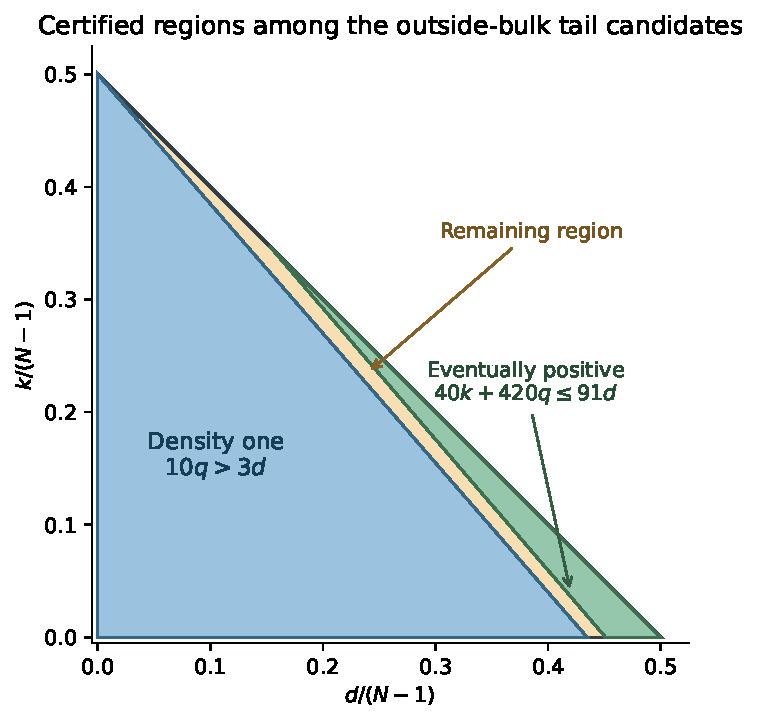
\includegraphics[width=.82\textwidth]{figures/37-global-049-regions.pdf}
\caption{The tail candidate triangle in coordinates $(d/(N-1),k/(N-1))$. Its area is $1/8$. The two proved regions have areas $5/46$ and $169/19912$; the positive bulk of leading size $3N^2/8$ is not shown. The remaining region is unresolved and is not asserted to contain zeros.}
\label{aud:gh:regions}
\end{figure}
\subsection{An exact contour and the favored critical curve}
Put
\[
 b=q-2d,\qquad \kappa=k/d,\qquad \delta=b/d,\qquad r=4+\delta.
\]
The coefficient has the exact single-contour representation~\eqref{aud:dc:actionintegral} with the action~\eqref{aud:dc:L}, whose $4+\delta$ is $r$. Manuscript~37 derives it by the same substitution $\omega=\mathrm e^t-1$, with $R=rd+1$. The original integer powers make the integrand single-valued despite the local logarithms, and its other poles are at $2\pi i\mathbb Z\setminus\{0\}$.

For the horizontal construction assume $\delta>-17/10$, $\delta\ne0$; the real-saddle region will be treated separately in Theorem~\ref{aud:gh:positivecone}. Write $\mathrm e$ for Euler's number. For modulus estimates let
\[
 e=|\delta|/2,\qquad h=r/2-e>0.
\]
The left half-plane is favored when $\delta>0$, and the right half-plane when $\delta<0$. Reflecting the real coordinate reduces both modulus problems to
\begin{equation}\label{aud:gh:centered}
 L_c(t)=\log t-et+\kappa\log\cosh(t/2)
                 -(\kappa+r)\log\sinh(t/2)-r\log2.
\end{equation}
For positive offsets, $h=2$ and $e=\delta/2$. For negative offsets,
\begin{equation}\label{aud:gh:reflection}
 h=2+\delta\in(0,2),\qquad r=h+2,\qquad e=(2-h)/2.
\end{equation}
Reflection sends a lower-left critical point of~\eqref{aud:gh:centered} to the original lower-right critical point and preserves real action values.

Write $t=-s-iy$ with $s>0$, $0<y<\pi$. Define
\begin{equation}\label{aud:gh:U}
 \mathcal U(s,y)=\frac{s\coth s-y\cot y}{s^2+y^2}
 =2\sum_{n\ge1}\frac{(n\pi)^2}
 {(s^2+(n\pi)^2)((n\pi)^2-y^2)}.
\end{equation}
The identity follows from the classical partial fractions~\cite{hyperbolic,trigonometric}. The series and its derivatives converge locally uniformly. In particular
\[
 \mathcal U_s<0,\qquad \mathcal U_y>0,
\]
while $\mathcal U(s,0)$ decreases from $1/3$ to zero and $\mathcal U(s,y)\to\infty$ as $y\uparrow\pi$.

The critical equation is $F_{r,e}(t)=\kappa$, where
\[
 F_{r,e}(t)=\frac{\sinh t}{t}-\frac r2(1+\cosh t)-e\sinh t.
\]
Its imaginary part factors as
\begin{equation}\label{aud:gh:imaginary}
 \operatorname{Im}F_{r,e}(-s-iy)
 =\sinh s\sin y\left\{\mathcal U(s,y)-h+\frac{2e}{\mathrm e^{2s}-1}\right\}.
\end{equation}
Assume $e>0$, as will hold off the line $\delta=0$. The right side of
\begin{equation}\label{aud:gh:heightcurve}
 \mathcal U(s,y)=h-\frac{2e}{\mathrm e^{2s}-1}
\end{equation}
increases from $-\infty$ to $h>0$. It first meets $\mathcal U(s,0)$ at a unique $s_0>0$. For $s>s_0$ there is one smooth curve $y(s)\in(0,\pi)$, strictly increasing from zero to $\pi$.

Along this curve,
\[
 \operatorname{Re}F_{r,e}'(-s-iy)=-\sinh s\sin y\,\mathcal U_y<0.
\]
The Cauchy--Riemann equations therefore give
\begin{equation}\label{aud:gh:CR}
 \kappa'(s)=-\operatorname{Re}F_{r,e}'(-s-iy)(1+y'(s)^2)>0,
 \qquad \kappa(s)=\operatorname{Re}F_{r,e}(-s-iy(s)).
\end{equation}
Also $\kappa(s)\to\infty$: as $y\to\pi$, the positive real term grows with leading size $he^s/2$, whereas the term $\sinh t/t$ is smaller by a factor $O(1/s)$. A point on the curve with negative $\kappa$ therefore ensures one simple favored critical point for each $\kappa\ge0$ at all later heights.

\subsection{A rational lower bound on the saddle height}
The next step supplies a uniform geometric condition for global contour selection.

\begin{lemma}[The saddle stays above height $\pi/2$]\label{aud:gh:height}
For every $\kappa\ge0$ and $\delta>-17/10$, $\delta\ne0$, there is a unique simple favored critical point in the lower strip $-\pi<\operatorname{Im}t<0$. Its height is strictly greater than $\pi/2$.
\end{lemma}
\begin{proof}
Set $C=\cosh s$, $S=\sinh s$, $c=\cos y$, and $\Sigma=s^2+y^2$. Eliminating $e$ from the imaginary critical equation gives the exact identity
\begin{equation}\label{aud:gh:elimination}
 \frac\kappa{C+c}
 =\mathrm e^s\left\{\frac{s+y(\mathrm e^{-s}-c)/\sin y}{\Sigma}-h\right\}.
\end{equation}
For positive offsets $h=2$. The numerator inside braces, after subtracting $h\Sigma$, has derivative
\[
 1-\frac y{\sin y}\mathrm e^{-s}-2hs<1-\mathrm e^{-s}-s<0.
\]
At $y=\pi/2$ its value at $s=0$ is $y-2y^2<0$. Thus the point of the curve at this height has negative $\kappa$.

For negative offsets, use~\eqref{aud:gh:reflection} and put $a=\pi/2$. At height $a$, equation~\eqref{aud:gh:heightcurve} becomes
\begin{equation}\label{aud:gh:B}
 h=B_h(s):=2\mathrm e^{-2s}+(1-\mathrm e^{-2s})\frac{s\coth s}{s^2+a^2}.
\end{equation}
This decreases strictly from 2 to zero: $\mathcal U_s<0$ and
$\mathcal U(s,a)\le \mathcal U(0,a)=1/a^2<2$ make its derivative negative. At this height, the sign of $\kappa$ is the sign of
\[
 J(s)=a-\mathrm e^{-s}(s+2s^2+2a^2).
\]
Moreover
\[
 J'(s)=\mathrm e^{-s}(2s^2-3s+2a^2-1)>0,
\]
since the quadratic has discriminant $17-4\pi^2<0$.

Take $s_*=51/20$. The elementary bounds
\[
 \pi>157/50,\qquad \mathrm e^{51/10}>160,\qquad \mathrm e^{51/20}<13
\]
give
\begin{equation}\label{aud:gh:heightcertificate}
 B_h(s_*)<\frac1{80}+
 \frac{(51/20)(161/160)}{(51/20)^2+(157/100)^2}
 =\frac{267803}{896740}<\frac3{10}.
\end{equation}
Also
\[
 \mathrm e^{s_*}<13<\pi+\frac{3111}{100\pi},
\]
so $J(s_*)<0$. For the last comparison, $x+3111/(100x)$ decreases on $(3,22/7)$ and its value at $22/7$ exceeds 13 by $639/15400$. The exponential inequalities follow respectively from the positive Taylor sum through order 10 and the sum through order 4 plus a geometric tail. The accompanying verifier replays these rational certificates exactly.

If $h\ge3/10$, the solution $B_h(s)=h$ has $s<s_*$ and therefore $J(s)<0$. This proves that the height-$\pi/2$ crossing has negative $\kappa$ in both cases. Monotonicity~\eqref{aud:gh:CR} and the increasing height curve now give a unique critical point for every $\kappa\ge0$, with height above $\pi/2$. Simplicity follows from the strictly negative real part of $F_{r,e}'$ in~\eqref{aud:gh:CR}.
\end{proof}

\subsection{Global selection on horizontal contours}
\begin{lemma}[A unique maximum on each horizontal line]\label{aud:gh:horizontal}
At a favored critical point of height $y\in(\pi/2,\pi)$, the lower horizontal line has exactly one global modulus maximum, at that point. The upper line has its conjugate maximum. Both maxima have nondegenerate horizontal curvature.
\end{lemma}
\begin{proof}
In the reflected favored model, put $J_y(s)=\operatorname{Re}L_c(-s-iy)$. Differentiation gives
\begin{equation}\label{aud:gh:horizontalderivative}
 J_y'(s)\frac{C-c}{S}
 =A_h(s)+eB_0(s)-\frac r2-\frac{\kappa c}{C+c},
\end{equation}
where
\[
 A_h(s)=\frac{s(C-c)}{(s^2+y^2)S},\qquad B_0(s)=\frac{C-c}{S}.
\]
Every variable term on the right decreases when $c<0$. For $A_h$, the partial fraction identity gives
\begin{equation}\label{aud:gh:periodic}
 \frac1{A_h(s)}=2\sum_{n\in\mathbb Z}
                 \frac{s^2+y^2}{s^2+(y+2\pi n)^2}.
\end{equation}
The $n=0$ term is constant. Every other term increases strictly with $s$, since $|y+2\pi n|>y$ for $0<y<\pi$. Hence $A_h$ decreases strictly. Also
\[
 B_0'(s)=\frac{C\cos y-1}{S^2}<0,
\]
and the last term in~\eqref{aud:gh:horizontalderivative} is decreasing because $c<0$.

The right side of~\eqref{aud:gh:horizontalderivative} tends to $+\infty$ at zero, due to $e>0$, and to $e-r/2=-h<0$ at infinity. It has one zero, and its derivative there is negative. The classified saddle is therefore the unique favored-side maximum, with $J_y''<0$. At the opposite point of real coordinate $s$, the action's real part is smaller by $2es$. Thus the maximum is unique on the whole horizontal line. Reflection returns the same assertion in the original coordinates, where
\[
 \operatorname{Re}(-L''(t_s))>0.
\]
\end{proof}

The small contour in~\eqref{aud:dc:actionintegral} can be enlarged to the boundary of $|\operatorname{Im}t|\le y$, with vertical sides tending to infinity. Since $y<\pi$, no other pole is enclosed. On the ends, uniformly on compact parameter sets,
\[
 \operatorname{Re}L(t)\le\log(1+|\operatorname{Re}t|)
                         -h|\operatorname{Re}t|+C.
\]
Thus the vertical integrals vanish. Uniqueness and compactness give a uniform gap away from the two saddle neighborhoods; the negative horizontal Hessian supplies uniform Gaussian decay there. This is a global selection argument, not a conclusion from the critical equation alone.

\begin{theorem}[Global compact-uniform cosine law]\label{aud:gh:cosine}
For the original lower favored saddle $t_s$, put
\begin{gather}
 W=-L''(t_s),\qquad
 P_h=\frac{-i}{4\sinh^2(t_s/2)\sqrt W},\qquad
 \Theta=d\operatorname{Im}L(t_s)+\arg P_h,\label{aud:gh:prefactor}\\
 \mathcal A_h=\frac{2M!}{d!\sqrt{2\pi d}}
                   \mathrm e^{d\operatorname{Re}L(t_s)}|P_h|>0.
\end{gather}
The square root has positive real part. On every compact subset of
$\kappa\ge0$, $\delta>-17/10$, $\delta\ne0$,
\begin{equation}\label{aud:gh:cosinelaw}
 H_{d,k,2d+b}=\mathcal A_h\bigl(\cos\Theta+O(d^{-1})\bigr)
\end{equation}
uniformly as $d\to\infty$. The error is additive, including at leading cosine zeros.
\end{theorem}
\begin{proof}
On the lower horizontal line, $dt=dx$. Its local Gaussian contribution, before multiplication by $M!/d!$, is
\[
 \mathrm e^{dL(t_s)}\frac{1}{4\sinh^2(t_s/2)}
                       \sqrt{\frac{2\pi}{dW}}\,(1+O(d^{-1})).
\]
The counterclockwise rectangle traverses the lower line from left to right and the upper line from right to left. The upper integral is the conjugate of the lower one. Division by $2\pi i$ therefore extracts the lower imaginary part, giving precisely the factor $-i$ in~\eqref{aud:gh:prefactor}.

The rate follows by expanding the local analytic exponent through its cubic term and the prefactor through its linear term on a symmetric interval. Odd Gaussian terms vanish. The remaining normalized moments of $x^2$, $dx^4$, and $d^2x^6$ are $O(d^{-1})$. The other arcs are exponentially small by Lemma~\ref{aud:gh:horizontal}. Summing the conjugate contributions yields~\eqref{aud:gh:cosinelaw}; no phase is divided out.
\end{proof}

At the regular boundary $\delta=0$, $t_s=-iT$ and
$\sqrt{t_s^2L''}=it_s\sqrt{-L''}$. Thus~\eqref{aud:gh:prefactor} agrees with the circular prefactor $t_s/(4\sinh^2(t_s/2)\sqrt{t_s^2L''})$, including its positive-imaginary base value. This checks the differential and orientation factors.

\subsection{From the phase law to density in the wide cone}
The action and nonzero prefactor are analytic on each of the two connected regions
\[
 \mathcal W_+=\{\kappa>0,\delta>0\},\qquad
 \mathcal W_-=\{\kappa>0,-17/10<\delta<0\}.
\]
The critical curve is unique and simple, and the logarithms can be chosen continuously in the lower strip. Consider the directional phase curvature
\begin{equation}\label{aud:gh:curvature}
 C(\kappa,\delta)=(\partial_\kappa-2\partial_\delta)^2
                          \operatorname{Im}L(t_s).
\end{equation}
It is not identically zero in either region. To check this directly, let $K(T)$ and $F(T)$ be~\eqref{aud:fr:K} and~\eqref{aud:fr:FD}.

At $T=14/5$, alternating Taylor bounds give $K(T)>0$ and $F(T)>0$, so $t_s=-iT$ is a nondegenerate base saddle with $L^{\prime\prime}(t_s)<0$. Its continuation enters the favored half-plane on each side of $\delta=0$, since $\operatorname{Re}(\partial_\delta t_s)=1/(2L^{\prime\prime}(t_s))<0$. Since the action is affine in $\kappa,\delta$ and
\[
 L_{t\kappa}-2L_{t\delta}=1+\coth t,
\]
stationary differentiation gives
\[
 (\partial_\kappa-2\partial_\delta)^2L(t_s)
 =-\frac{(1+\coth t_s)^2}{L''(t_s)}.
\]
At $t_s=-iT$ its imaginary part is $2T^2\cos T/F(T)<0$. The analytic continuations from positive and negative $\delta$ have this same nonzero limit.

\mergenote{Manuscript~40's formula~\eqref{aud:dc:curvature} gives this value on the whole regular branch, and it is negative there. The integer-point estimate used next is Lemma~\ref{aud:sc:lattice}. Manuscript~37 states and proves the same lemma, and it is printed once.}


On a compact parameter rectangle where $|C|$ is bounded away from zero, interpolate at fixed $N,d$
\[
 f_{d,N}(X)=\frac1\pi\left[d\operatorname{Im}L\left(t_s\left(\frac Xd,
 \frac{N-1-4d-2X}{d}\right)\right)+\arg P_h\right]-\frac12.
\]
Its second derivative is bounded between fixed nonzero multiples of $1/d$ in one sign; the prefactor argument contributes only $O(d^{-2})$. If $H=0$, the additive cosine law forces $\operatorname{dist}(f_{d,N}(k),\mathbb Z)=O(d^{-1})$. Lemma~\ref{aud:sc:lattice} then gives $O(d^{2/3})$ zeros per row, hence $O(N^{5/3})$ over any such fixed patch.

To remove the curvature restriction on a compact patch, use real analyticity. The zero set of the nonzero analytic function $C$ has area zero, by the elementary argument in the proof of Theorem~\ref{aud:dc:density}, which manuscript~37 repeats.

The exact ratio map is
\begin{equation}\label{aud:gh:Jacobian}
 x=\frac d{N-1}=\frac1{4+2\kappa+\delta},\qquad
 y=\frac k{N-1}=\frac\kappa{4+2\kappa+\delta},\qquad
 \left|\frac{\partial(x,y)}{\partial(\kappa,\delta)}\right|
 =(4+2\kappa+\delta)^{-3}.
\end{equation}
For a fixed finite union $\Omega$ of compact rectangles inside $\mathcal W_+\cup\mathcal W_-$, the image has piecewise smooth boundary. Its candidate count is
\begin{equation}\label{aud:gh:compactcount}
 (N-1)^2I_\Omega+O_\Omega(N),\qquad
 I_\Omega=\int_\Omega(4+2\kappa+\delta)^{-3}\,d\kappa\,d\delta.
\end{equation}
Cover the compact image of $\{C=0\}$ by finitely many open boxes of total area less than $\epsilon$. They contain at most $\epsilon(N-1)^2+O_\epsilon(N)$ lattice candidates. The remaining compact set has a finite cover by curvature rectangles, on which the zero count is $O_\epsilon(N^{5/3})$. Taking $N\to\infty$ first and then $\epsilon\downarrow0$ proves $o(N^2)$ exact cancellations in $\Omega$.

Finally exhaust $\mathcal W_+\cup\mathcal W_-$ by finite unions of compact rectangles, for example
\[
 \kappa\in[1/m,m],\qquad
 \delta\in[-17/10+1/m,-1/m]\cup[1/m,m].
\]
Their integrals increase to
\begin{equation}\label{aud:gh:widearea}
 \int_0^\infty\int_{-17/10}^\infty
       (4+2\kappa+\delta)^{-3}\,d\delta\,d\kappa=\frac5{46}.
\end{equation}
There is no uniform analytic error claim over this noncompact set. For each fixed exhaustion set first take the limit in $N$, and only then enlarge the set.

For completeness this also gives the global $o(N^2)$ cancellation count in the stated cone. The full cone $10q>3d$ is, in $(x,y)$ coordinates, the triangle
\[
 x\ge0,\quad y\ge0,\quad (23/10)x+2y<1,
\]
with $5/46$ area and $O(N)$ lattice boundary error. Outside any fixed exhaustion set, the candidate count divided by $N^2$ has limsup at most $5/46-I_\Omega$. Letting $\Omega$ exhaust proves that the whole cone has only $o(N^2)$ exact zeros. This is a qualitative global density statement; the $O(N^{5/3})$ estimate was used only on fixed curvature patches. The line $\delta=0$ and coordinate boundaries have zero area and are harmless in this argument.
\subsection{Angular selection below radius three}\label{aud:gh:angularsection}
We need a second contour argument for a disjoint region near $q=0$.
It gives a positive real saddle rather than an oscillating conjugate pair.
Throughout this section, $L$ is the leading action in~\eqref{aud:dc:L}.

\begin{lemma}[A positive real saddle is globally selected]\label{aud:gh:angularselection}
Suppose $\kappa\ge0$, $-2\le\delta<0$, and $T\in(0,3]$ satisfies
\[
 L'(T)=0,\qquad V=T^2L''(T)>0.
\]
Then $t=T$ is the unique global maximum of $\operatorname{Re}L(t)$ on
$|t|=T$.  On a compact family of such saddles, the resulting one-arc
asymptotic is uniform:
\begin{equation}\label{aud:gh:realasymptotic}
 H_{d,k,q}=
 \frac{M!}{d!}\,\mathrm e^{dL(T)}
 \frac{T}{4\sinh^2(T/2)\sqrt{2\pi dV}}
 \bigl(1+O(d^{-1})\bigr).
\end{equation}
In particular the coefficient is strictly positive for sufficiently large
$d$, uniformly on the compact family.
\end{lemma}
\begin{proof}
Put $c=(T/\pi)^2$.  Since $T\le3$ and $\pi>157/50$, we have $0<c<23/25$.
The hyperbolic products give the factors
\[
 a(x)=\frac{4cx^2}{(x^2-c)^2},\qquad
 A_n=a(2n-1),\qquad B_n=a(2n).
\]
For $0\le z\le1$ define their transformed version
\[
 a_z(x)=\frac{a(x)}{1+za(x)}
       =\frac{4cx^2}{x^4+(4z-2)cx^2+c^2}.
\]
It is strictly decreasing for $x\ge1$: its logarithmic first derivative
has numerator $2(c^2-x^4)$.  We claim that the ratios
$a_z(2n-1)/a_z(2n)$ are nonincreasing in $n$.

First, writing $D_z(x)=x^4+(4z-2)cx^2+c^2$, differentiation gives
\[
 (\log a_z)''(x)=\frac{2}{x^2D_z(x)^2}
 \left\{x^8+(2-4z)cx^6-8c^2x^4+(6-12z)c^3x^2-c^4\right\}.
\]
For $x\ge3$, the numerator in braces is bounded below by
\[
 x^8-2x^6-8x^4-6x^2-1
 \ge x^8\left(1-\frac29-\frac8{81}-\frac6{729}-\frac1{6561}\right)>0.
\]
Thus logarithmic convexity proves the claim for the successive ratios
starting with $n=2$.  The remaining first comparison is exact algebra:
\begin{gather*}
 a_z(1)a_z(4)-a_z(2)a_z(3)
 =\frac{-64c^2Q(c,z)}{D_z(1)D_z(2)D_z(3)D_z(4)},\\
 Q(c,z)=5c^4+(404z-202)c^3+1925c^2+(2304z-1152)c-2880.
\end{gather*}
The polynomial $Q$ increases with $z$.  Moreover
\[
 Q(c,1)=5c^4+202c^3+1925c^2+1152c-2880
\]
is increasing for $c>0$, and its value at $23/25$ is
$-2340864/78125<0$.  All denominators are positive.  This proves the
claimed transformed ratio ordering.

Set
\[
 S_A(z)=\sum_{n\ge1}\frac{A_n}{1+A_nz},\qquad
 S_B(z)=\sum_{n\ge1}\frac{B_n}{1+B_nz},\qquad \varrho(z)=\frac{S_A(z)}{S_B(z)}.
\]
Normalize the two summand sequences to probabilities $p_n,q_n$.  Their
likelihood ratio is nonincreasing in $n$.  Since $a_z(2n-1)$ decreases,
the elementary covariance comparison yields
\[
 \mathbb E_p a_z(2n-1)\ge\mathbb E_q a_z(2n-1)
                       >\mathbb E_q a_z(2n).
\]
Termwise differentiation is justified by absolute convergence, and therefore
\begin{equation}\label{aud:gh:Rdecreases}
 \frac{\varrho'(z)}{\varrho(z)}
 =-\mathbb E_p a_z(2n-1)+\mathbb E_q a_z(2n)<0.
\end{equation}

A further elementary bound will control the tilt.  The function
$h_B(z)=\sqrt z\,S_B(z)$ is strictly increasing for $0<z\le1$, because
\[
 2\sqrt z\,h_B'(z)
 =\sum_{n\ge1}\frac{B_n(1-B_nz)}{(1+B_nz)^2}>0.
\]
Here is an explicit verification of the strict sign.  For $n=1$,
$B_1/c\le16/9$ and $B_1z\le16/9$, so its summand is at least
$-112c/625$.  For $n\ge2$,
\[
 \frac c{n^2}\le B_n\le\frac{64}{225},\qquad
 \frac{1-B_nz}{(1+B_nz)^2}\ge\frac{36225}{83521}.
\]
Using $\sum_{n\ge2}n^{-2}>1/2$, already true of the terms $2\le n\le7$,
we obtain
\begin{equation}\label{aud:gh:hincreases}
 2\sqrt z\,h_B'(z)
 \ge c\left(\frac{36225}{167042}-\frac{112}{625}\right)>0.
\end{equation}

Write $\nu=-\delta>0$ and $r=4+\delta>0$.  On a quadrant in the positive
half-circle, use $z=(\operatorname{Re}t/T)^2$.  Up to a constant, the real
action is
\[
 G(z)=\frac\kappa2\sum\log(1+A_nz)
       -\frac{\kappa+r}{2}\sum\log(1+B_nz)
       +\frac{\nu T}{2}\sqrt z.
\]
Its derivative has the sign of
\begin{equation}\label{aud:gh:anglesign}
 \kappa\varrho(z)-(\kappa+r)+\frac{\nu T}{2h_B(z)},
\end{equation}
which is strictly decreasing by~\eqref{aud:gh:Rdecreases}--\eqref{aud:gh:hincreases}.
At the real saddle, the expansion $z=\cos^2\theta=1-\theta^2+O(\theta^4)$
gives $G'(1)=V/2>0$.  Thus~\eqref{aud:gh:anglesign} is positive on $(0,1]$,
and $G$ is strictly increasing.  Every point in the negative half-circle
has smaller real action than its reflected positive-half point, by
$\nu|\operatorname{Re}t|$.  The imaginary points are also smaller than
$T$.  Hence $T$ is the unique global maximum.

The circle has radius less than $\pi$, so the exact contour can be enlarged
to it without crossing another pole.  On compact saddle families,
strict global dominance and $V>0$ give uniform far-arc suppression and
local Gaussian decay.  In $t=Te^{i\theta}$, the Cauchy differential supplies
$T$, and the analytic factor is $1/(4\sinh^2(T/2))$.  The single Gaussian
integral gives~\eqref{aud:gh:realasymptotic}; there is no conjugate-pair factor
of two.  Odd local terms integrate to zero and the next normalized moments
are $O(d^{-1})$.  Every leading factor in~\eqref{aud:gh:realasymptotic} is
positive.
\end{proof}

\subsection{An explicit positive coefficient cone}\label{aud:gh:conesection}
\begin{theorem}[Uniform eventual positivity]\label{aud:gh:positivecone}
For every sufficiently large integer $d$, uniformly over all integers
$k,q\ge0$ satisfying
\begin{equation}\label{aud:gh:coneinequality}
 40k+420q\le91d,
\end{equation}
one has $H_{d,k,q}>0$.  The threshold is uniform but is not claimed to be
numerical.
\end{theorem}
\begin{proof}
Put $\eta=q/d=\delta+2$.  The scaled parameter triangle is
\[
 \kappa\ge0,\qquad\eta\ge0,\qquad40\kappa+420\eta\le91.
\]
In particular $0\le\eta\le13/60$, so $\delta<0$.  On the positive real axis,
the critical equation is $F_\delta(T)=\kappa$, with
\begin{gather*}
 F_\delta(T)=\frac{\sinh T}{T}-\mathrm e^{-T}-1
                  -\frac\eta2(1+\mathrm e^T)
             =\frac{1+\mathrm e^T}{2}\bigl(g(T)-\eta\bigr),\\
 g(T)=\frac{1-\mathrm e^{-T}}{T}-2\mathrm e^{-T}.
\end{gather*}
For $0<T\le3$,
\[
 g'(T)=\frac{\mathrm e^{-T}(2T^2+T+1)-1}{T^2}>0.
\]
Indeed, the positive Taylor series makes $(\mathrm e^T-1-T)/T^2$ increasing, and
at $T=3$ its value is $(\mathrm e^3-4)/9<17/9<2$, using $\mathrm e^3<21$.

At $T=1$,
\[
 F_\delta(1)\le\frac{(\mathrm e-3)(\mathrm e+1)}{2\mathrm e}<0.
\]
At $T=3$, put $E_3=\mathrm e^3>20$.  Since $\eta\le13/60<1/3$,
\begin{align*}
 F_\delta(3)
 &=E_3\left(\frac16-\frac\eta2\right)-\frac7{6E_3}-1-\frac\eta2\\
 &>\frac{91}{40}-\frac{21}{2}\eta\ge\kappa.
\end{align*}
Once $F_\delta\ge0$, its derivative is strictly positive by the factored
form and $g'>0$.  There is consequently exactly one saddle $T\in(1,3)$
at every parameter point of the triangle.  At this saddle,
\[
 V=T^2L''(T)=\frac{T^2F_\delta'(T)}{\sinh T}>0.
\]
The strict endpoint inequalities, compactness of the triangle, and the
implicit function theorem make the radius bounds and positive curvature
uniform, including $\kappa=0$ and $\eta=0$.  Apply
Lemma~\ref{aud:gh:angularselection} to obtain the uniform positivity.
\end{proof}

\begin{corollary}[Additional positive terms]\label{aud:gh:positivearea}
At derivative order $N$, the cone~\eqref{aud:gh:coneinequality} supplies
\begin{equation}\label{aud:gh:trianglecount}
 \frac{169}{19912}(N-1)^2+O(N)
\end{equation}
nonzero monomials outside the proved positive bulk.  These cells are also
disjoint from the oscillatory region $q/d>3/10$.
\end{corollary}
\begin{proof}
Set $x=d/(N-1)$ and $y=k/(N-1)$.  The exact bridge
$N-1=2k+2d+q$ turns the conditions into a fixed triangle with vertices
\[
 \left(\frac12,0\right),\qquad
 \left(\frac{420}{931},0\right),\qquad
 \left(\frac{20}{131},\frac{91}{262}\right).
\]
Its area is
\[
 \frac12\left(\frac12-\frac{420}{931}\right)\frac{91}{262}
 =\frac{169}{19912}.
\]
The grid-point count has this area times $(N-1)^2$, with boundary error
$O(N)$.  Every depth is comparable to $N$, so Theorem~\ref{aud:gh:positivecone}
applies to all these cells once $N$ is large.  Excluding the edge $q=0$
removes only $O(N)$ already-bulk cells.  For the others, $j=-q-1\le-2$,
and the factor $\binom Nk$ in the coefficient bridge is positive.  At fixed
$N$, the coordinates $(j,k)$ determine $d$, so distinct cells give distinct
monomials.  Finally $q/d\le13/60<3/10$, proving disjointness from the
oscillatory region.
\end{proof}

\subsection{Combining the regions and the remaining question}
The positive-real triangle has $\delta\le-2+91/420<-17/10$, so it is disjoint from the wide oscillatory cone. Its $q=0$ boundary belongs to the earlier bulk and contributes only $O(N)$ cells. All other counted cells have $q\ge1$, hence $j\le-2$; injectivity of~\eqref{aud:bridge} prevents double counting.

The wide cone contributes $(5/46)N^2+o(N^2)$ nonzero terms, and the positive-real triangle contributes $(169/19912)N^2+O(N)$ for all sufficiently large $N$. Adding~\eqref{aud:bulk} proves~\eqref{aud:gh:constant}. The exact excess over $49/100$ is
\[
 \frac{28176}{57247}-\frac{49}{100}=\frac{12497}{5724700}>0.
\]
This strict margin gives the eventual pointwise inequality in Theorem~\ref{aud:gh:main}.

The proof does not establish exact noncancellation in the oscillatory cone, determine every coefficient in the intervening region, or prove $a(N)\sim N^2/2$. \addednote{the leading asymptotic $a(N)=N^2/2+o(N^2)$ was proved the same day by manuscript~34, written after this manuscript, and is printed in the sibling report \emph{power-tower-exponent-supports}~\cite{pte}. That theorem is ineffective, so the explicit bounds of the source and of its batch-72A count-bounds addition remain the best effective ones (Section~\ref{aud:sec:headlines}). The full support conjecture remains open.} The full tail candidate area is $1/8$; the two regions proved here have total area $5/46+169/19912$. Figure~\ref{aud:gh:regions} displays the remaining gap.

The result and its complete proofs received independent mathematical review. The accompanying rational verifier checks all elementary Taylor, angular-selection, and area certificates; finite numerical experiments are not used to prove the saddle or density assertions. The arguments have not been formalized in Lean or externally refereed, and no exhaustive priority claim is made.
\section{A pointwise three-halves correction (manuscript 53)}\label{aud:sec:53b}
This section derives manuscript~53's count from its growing-offset phase law, Theorem~\ref{aud:go:uniform} and Corollary~\ref{aud:go:safecells} (Section~\ref{aud:sec:53a}).

\begin{theorem}[Pointwise three-halves correction; superseded, see Section~\ref{aud:sec:headlines}]\label{aud:go:main}
There are constants $C>0$ and $N_0$ such that, for every integer $N\ge N_0$,
\begin{equation}\label{aud:go:mainbound}
 a(N)\ge\beta(N)+CN^{3/2}\ge\frac38N^2+CN^{3/2}.
\end{equation}
\end{theorem}

This is a pointwise bound, not a summatory or average statement. Neither a numerical value of $C$ nor a numerical threshold $N_0$ is claimed. The leading quadratic coefficient remains $3/8$; no conjectural $N^2/2$ asymptotic is inferred. \addednote{the leading coefficient of the pointwise lower bound was already above $3/8$ by manuscript~49 (Theorem~\ref{aud:qg:count}), and $a(N)=N^2/2+o(N^2)$ is manuscript~34\textquoteright s theorem~\cite{pte}; see Section~\ref{aud:sec:headlines}.}
\subsection{Counting a positive fraction of phase-safe depths}
We now use the proved growing-offset phase estimate to count terms at each derivative order. Fix
\[
 I=[\kappa_-,\kappa_+]=[1/100,1/50]\subset(0,\kappa_c).
\]
The phase-safe consequence~\ref{aud:go:safecells} supplies constants $\eta_*>0$ and $d_*$ such that, for $d\ge d_*$, $k/d\in I$, $1\le b\le\eta_*\sqrt d$, and $\varepsilon=0$,
\begin{equation}\label{aud:go:safesufficient}
 |\cos(b\psi(k/d))|\ge\frac12
 \quad\Longrightarrow\quad H_{d,k,2d+b}\ne0.
\end{equation}
Indeed choose $\eta_*$ so that the normalized error is at most $1/4$ for large $d$. Shrink $\eta_*$ further if necessary so that $\eta_*\le1$.

Define the positive constants
\begin{equation}\label{aud:go:countconstants}
 \Delta\psi=\psi(\kappa_-)-\psi(\kappa_+)>0,\qquad
 G=\max_{\kappa\in I}\frac{(\kappa+2)^2}{2K'(t(\kappa))}<\infty.
\end{equation}
Their positivity and finiteness follow from the strictly positive derivative of the regular branch on $I$.

\begin{lemma}[Phase-safe depths with the required parity]\label{aud:go:depthcount}
Fix a derivative order $N$ and a positive integer $b$ with $b\equiv N-1\pmod2$. Put $n_b=(N-1-b)/2$. If
\[
 b\ge B_0:=\left\lceil\frac{6\pi}{\Delta\psi}\right\rceil,
\]
then the number of integer depths $d$ satisfying
\[
 \frac{k}{d}\in I,\qquad k=n_b-2d,\qquad
 \varepsilon=0,\qquad |\cos(b\psi(k/d))|\ge\frac12
\]
is at least
\begin{equation}\label{aud:go:depthlower}
 \frac{n_b\Delta\psi}{6G}-2-\frac{2b\Delta\psi}{\pi},
\end{equation}
provided $n_b>0$.
\end{lemma}
\begin{proof}
The real depths with $\kappa(d)=k/d=n_b/d-2\in I$ form the interval
\[
 J_{N,b}=\left[\frac{n_b}{\kappa_++2},\frac{n_b}{\kappa_-+2}\right].
\]
On it, $\theta_b(d)=b\psi(\kappa(d))$ increases strictly through an angle interval of length $b\Delta\psi$. Differentiating $\psi(\kappa)=(\pi-t(\kappa))/2$ gives
\[
 \theta_b'(d)=\frac{b(\kappa(d)+2)^2}{2n_bK'(t(\kappa(d)))}
 \le\frac{bG}{n_b}.
\]
In an arbitrary real interval of length $L$, the set where $|\cos\theta|\ge1/2$ has measure at least $(2/3)L-2\pi$. For $b\ge B_0$, this is at least $b\Delta\psi/3$. Its preimage in $J_{N,b}$ consequently has total length at least $n_b\Delta\psi/(3G)$.

The safe phase set has at most $2+2b\Delta\psi/\pi$ connected components; monotonicity gives the same bound for its preimage. Meanwhile
\[
 d-k-1=3d-n_b-1,
\]
so the exact parity requirement $\varepsilon=0$ is
\begin{equation}\label{aud:go:depthparity}
 d\equiv n_b+1\pmod2.
\end{equation}
Each real interval of length $\ell$ contains at least $\ell/2-1$ integers in this prescribed parity class. Summing over the components proves~\eqref{aud:go:depthlower}. This is interval counting and requires no equidistribution assumption.
\end{proof}

\begin{theorem}[A pointwise correction of order $N^{3/2}$]\label{aud:go:pointwisecount}
There exist constants $C>0$ and $N_0$ such that, for every integer $N\ge N_0$,
\begin{equation}\label{aud:go:maincount}
 a(N)\ge\beta(N)+CN^{3/2}\ge\frac38N^2+CN^{3/2},
\end{equation}
where
\[
 \beta(N)=\begin{cases}
 (3N^2+10N+8)/8,&N\text{ even},\\
 (3N^2+12N+1)/8,&N\text{ odd}
 \end{cases}
\]
is the established positive-bulk count. In terms of~\eqref{aud:go:countconstants} and the analytic choice of $\eta_*$, any positive $C$ smaller than
\begin{equation}\label{aud:go:Cexpression}
 \frac{\eta_*\Delta\psi}{144\sqrt6\,G}
\end{equation}
may be used. Neither a numerical value of $\eta_*$ nor a numerical threshold $N_0$ is asserted.
\end{theorem}
\begin{proof}
Put $R_N=\eta_*\sqrt{N/6}$ and $B_N=\lfloor R_N\rfloor$. Keep the offsets
\begin{equation}\label{aud:go:offsetselection}
 B_0\le b\le B_N,\qquad b\equiv N-1\pmod2.
\end{equation}
For all sufficiently large $N$, one has $b\le\sqrt N$, $N-1-b\ge3N/4$, and hence $n_b\ge3N/8\ge N/3$. Every real depth in $J_{N,b}$ then satisfies
\[
 d\ge\frac{3N/8}{\kappa_++2}>\frac N6,
\]
because $\kappa_++2<9/4$. In particular
\[
 b\le\eta_*\sqrt{N/6}\le\eta_*\sqrt d,
\]
and $d\ge d_*$ once $N$ is large enough. Thus every phase-safe integer depth supplied by Lemma~\ref{aud:go:depthcount} meets the analytic hypotheses of~\eqref{aud:go:safesufficient}.

The error term in~\eqref{aud:go:depthlower} is $O(b+1)=O(\sqrt N)$, uniformly in the selected offsets. It follows that, for all sufficiently large $N$, each such $b$ supplies at least
\[
 \frac{N\Delta\psi}{36G}
\]
nonzero cells. Once $R_N\ge2B_0+6$, the number of offsets in~\eqref{aud:go:offsetselection} is at least $R_N/4$. Their product gives the following lower bound on nonzero cells:
\[
 \frac{\eta_*\Delta\psi}{144\sqrt6\,G}N^{3/2}.
\]

It remains to check that these are distinct new derivative terms. Their coordinates are
\begin{equation}\label{aud:go:bridgecount}
 q=2d+b\ge1,\quad
 k=\frac{N-1-b-4d}{2}\ge0,\quad
 j=-2d-b-1,\quad
 N=2k+4d+b+1.
\end{equation}
There are no reflection holes because $b>0$. If two pairs $(b,d)$ gave the same $(j,k)$, equality of $j$ would give $\Delta b+2\Delta d=0$, whereas equality of $k$ would give $\Delta b+4\Delta d=0$. Both differences must vanish. The resulting monomials are therefore distinct.

The source bulk consists of the nonnegative $x$-power columns and the positive $j=-1$ boundary. Our cells have $j\le-2$ and $d\ge1$, so they are outside that bulk. Equivalently, they occupy the disjoint tail region $d\ge1$, $q\ge1$. Adding the source bulk count proves~\eqref{aud:go:maincount}.
\end{proof}

The new cells have depths $d\ge N/6$. Consequently they are also disjoint, for large $N$, from any separately certified shallow-depth region with depth $O(\log N)$. The proof therefore does not replace or double-count such earlier contributions. The leading lower-bound coefficient remains $3/8$ \addednote{stale against manuscripts~49 and~34, see the previous note; the shallow-depth region with depth $O(\log N)$ alluded to is that of the source\textquoteright s Section~3.23 and of its batch-72A count-bounds addition (manuscript~68), which 53 does not cite}; the new unconditional pointwise improvement is the positive correction of order $N^{3/2}$.
\subsection{Scope, verification, and the remaining problem}
The new contribution is a pointwise lower bound at every sufficiently large derivative order. It is stronger than a pointwise correction of order $N\log N$, while remaining compatible with separate stronger summatory lower bounds. \addednote{the order-$N\log N$ correction and the summatory bounds are manuscript~68\textquoteright s, now an addition to the source report; manuscript~53 does not cite it.} The constant $C$ is positive by the proof, but the saddle threshold and an admissible numerical $\eta$ are not evaluated here.

The argument proves only selected coefficients nonzero. It does not prove the full support conjecture, does not identify the conjectured $N^2/2$ leading asymptotic, and does not claim exact zeros from phase crossings. The growing-offset estimate intentionally uses a uniform error of order $|b|/\sqrt d+b^2/d$; no fixed-$b$ $O(1/d)$ remainder is asserted in this report. \addednote{manuscript~45\textquoteright s Theorem~\ref{aud:sc:fixedrate} supplies that remainder at fixed $b$ (Section~\ref{aud:sec:45a}).}

The coefficient model and bulk region are credited to the inspected source. The regular saddle geometry is verified through the displayed identities, with its rational subinterval checked by exact fractions. All other arguments are analytic or elementary interval counting. The proof received independent mathematical review, including the full offset dependence and parity count. It has not been formalized in Lean or externally refereed, and no exhaustive priority claim is made.
\section{The headline lower bounds and what supersedes them}\label{aud:sec:headlines}
Each of the five manuscripts of this part ends in a pointwise lower bound for $a(N)$. Each bound holds for every $N\ge N_0$ with an $N_0$ that is not numerical, and each manuscript says so. Table~\ref{aud:tab:headlines} lists them.

{\small
\begin{longtable}{@{}>{\raggedright\arraybackslash}p{0.07\textwidth}
 >{\raggedright\arraybackslash}p{0.38\textwidth}
 >{\raggedright\arraybackslash}p{0.48\textwidth}@{}}
\caption{Headline lower bounds of Part~\ref{aud:part:III}, all ineffective and all implied by $a(N)=N^2/2+o(N^2)$ (manuscript~34,~\cite{pte}). The right column lists what each manuscript proves that a count asymptotic does not imply.}\label{aud:tab:headlines}\\
\toprule
MS & Headline bound & Kept here, not implied by the count asymptotic\\
\midrule\endfirsthead
\toprule
MS & Headline bound & Kept here, not implied by the count asymptotic\\
\midrule\endhead
37 & Theorem~\ref{aud:gh:main}(3): $\liminf a(N)/N^2\ge28176/57247=0.49218\ldots$, so $a(N)\ge0.49N^2$ eventually & the horizontal-contour cosine law on the wide cone (Theorem~\ref{aud:gh:cosine}) with its rational height certificate; uniform eventual positivity of \emph{every} coefficient on the triangle $40k+420q\le91d$ (Theorem~\ref{aud:gh:positivecone}), by real-saddle angular selection\\
49 & Theorems~\ref{aud:qg:main} and~\ref{aud:qg:count}: $a(N)\ge(3/8+c)N^2$; in fact $a(N)\ge\beta(N)+C_{\mathcal R}(N-1)^2-O(N)$ & the global inner-saddle bound, the two-saddle additive cosine law with explicit amplitude and phase (Theorem~\ref{aud:qg:cosine}), and the separated adjacent phases (Theorem~\ref{aud:qg:increment})\\
45 & Corollary~\ref{aud:sc:count}: $a(N)\ge\beta(N)+C_{\rm patch}(N-1)^2-O(N^{5/3})$, $C_{\rm patch}=4C_{\mathcal R}$ & the fixed-offset $O(1/d)$ rate and bounded strips (Section~\ref{aud:sec:45a}); the explicit negative row curvature~\eqref{aud:sc:negativecurvature}; $O(d^{2/3})$ zeros per row and $O(N^{5/3})$ per patch\\
40 & Corollary~\ref{aud:dc:stripdensity}: $a(N)\ge(3/8+C_0)N^2-O(N^{5/3})$; and $\liminf a(N)/N^2\ge3/8+\int_\Omega(4+2\kappa+\delta)^{-3}$ for every admissible patch & the cosine law through $\delta=0$ and $\kappa=0$ (Theorem~\ref{aud:dc:main}); the curvature $2T^2\cos T/F(T)<0$ on the whole branch~\eqref{aud:dc:curvature}; the odd--even product comparison (Lemma~\ref{aud:dc:comparison}); the density theorem for analytic exceptional sets (Theorem~\ref{aud:dc:density})\\
53 & Theorem~\ref{aud:go:main}: $a(N)\ge\beta(N)+CN^{3/2}$ & the phase law uniform in $|b|\le\sqrt d$ with explicit error (Theorem~\ref{aud:go:uniform})\\
\bottomrule
\end{longtable}}

\paragraph{The superseding relation.}
Manuscript~34 proves $a(N)/N^2\to1/2$; more precisely, the outside-bulk tail has only $o(N^2)$ exact zeros. Its proof is the $a=2$ case of manuscript~28's theorem for $x^{x^a}$, and both are printed in the sibling report \emph{power-tower-exponent-supports}~\cite{pte}. Every bound in Table~\ref{aud:tab:headlines} has leading constant at most $28176/57247<1/2$, so each holds for all sufficiently large $N$ as a consequence. Manuscript~34 asserts no numerical error rate or order threshold, so no effectivity is lost; the headline bounds were never effective either. Manuscript~34 does not imply the statements in the right column. Those are statements about individual coefficients: cosine laws, separated phases, positivity, bounded strips and curvature formulas. The density-one statements on fixed patches (45, 40, 37) overlap manuscript~34's own compact-patch argument, which uses the same integer-triangle lemma; manuscript~34 proves those patch statements away from the line $\delta=0$ only, which its argument discards as a set of zero area, while 40's strip contains that line. All five manuscripts were written before~34, and none cites it.

\paragraph{Effective bounds.}
The best effective lower bounds are not in this report. The source proves, for every $N\ge0$, the bulk count plus the classified cells of depths one to four (its Corollary \texttt{xxb:dc:cor:lower}). The batch-72A count-bounds addition to the source (manuscript~68, code shipped there as \nolinkurl{code/07-count-bounds-verify_counts.py}) proves
\[
 a(N)\ge\frac38N^2+\frac N2\log N-\frac N2\log\log N-\frac54N\qquad(N\ge e^{10}),
\]
and an exact summatory bound with cubic constant $11/72$. Manuscript~34's asymptotic implies neither.

\part{Arithmetic at unbounded deficit}\label{aud:part:IV}
Part~\ref{aud:part:IV} is manuscript~64, its Sections~1--4, 7 and~8; its Sections~5 and~6 are the case $\kappa=0$ in Part~\ref{aud:part:I}. Unlike Parts~\ref{aud:part:I}--\ref{aud:part:III}, its congruence families and central strips hold at every depth in the stated families, not only eventually.

In this part $r=2d+q+1$ and $M=k+r$, as in Section~\ref{aud:sec:model}. The polynomials $G_j(c,r)$ are~\eqref{aud:fr:G}; manuscript~64 wrote their variable as $a$, renamed $c$ here. Throughout, $p$ is an odd prime and $v_p$ the $p$-adic valuation. In Theorem~\ref{aud:ap:thm:blocks}, $r=Ap+s$ and $k=Bp+t$ with residues $s,t$, so $s$ is not $|b|$ there, and $C=A+B$.

\paragraph{Status and attribution.}
The results have ordinary mathematical proofs and reproducible exact checks, with independent mathematical review. They are not formally verified in Lean or externally refereed. Consecutive-factor congruences, the classical Meixner--Pollaczek framework, and Bernoulli local limit theory are credited inputs. The contribution is their stated application to these coefficient families, the exact valuations, and the central-strip and phase conclusions. Worldwide priority is not asserted.
\section{The scope of the arithmetic results (manuscript 64)}\label{aud:sec:apscope}

The desired full conjecture says that this integer vanishes precisely when $q=2d$ and $k+d$ is even. Those symmetry zeros are already proved; the converse is not assumed here.
The source report completes depths one through four; an earlier companion completes depths five and six and supplies exponential fixed-depth cutoffs \addednote{the companion is manuscript~70, now the batch-72A addition on depths five and six to the source report; manuscript~64 does not cite it}. The present families allow the depth itself to grow without bound. They do not classify every cell at any further complete depth.
\section{A block congruence for the centered recurrence}
The calculations in this section use classical finite-field algebra. The underlying consecutive-factor congruence is the standard mechanism behind Stirling congruences; compare~\cite{guillot}. We give all needed proofs.

\begin{lemma}[A prime-length recurrence block]\label{aud:ap:lem:Gp}
For every odd prime $p$,
\begin{equation}\label{aud:ap:eq:Gp}
 G_p(c,r)\equiv c^p-c\pmod p
\end{equation}
as a polynomial in $c,r$. Consequently, for $B\ge0$ and $0\le t<p$,
\begin{equation}\label{aud:ap:eq:Gblocks}
 G_{Bp+t}(c,r)\equiv(c^p-c)^B G_t(c,r)\pmod p.
\end{equation}
\end{lemma}
\begin{proof}
First fix $c,r\in\mathbb F_p$. Choose representatives $A_0,B_0\in\{0,\ldots,p-1\}$ satisfying $A_0-B_0=c$ and $-(A_0+B_0)=r+1$ in the field. This is possible because two is invertible. The polynomial
\[
 Y_p(z)=(1+z)^{A_0}(1-z)^{B_0}
\]
satisfies $(1-z^2)Y_p'=(c+(r+1)z)Y_p$. Its derivatives at zero satisfy~\eqref{aud:fr:G}, so $G_p(c,r)=Y_p^{(p)}(0)=0$ in characteristic $p$. For fixed $r$, monicity and degree $p$ in $c$ imply~\eqref{aud:ap:eq:Gp}. Every coefficient has degree at most $(p-1)/2$ in $r$, by the recurrence; agreement at all $r\in\mathbb F_p$ therefore proves the polynomial identity.

At an index $Bp$, the recurrence multiplier $j(j+r)$ vanishes modulo $p$. The following block restarts from a scalar multiple of $G_0,G_1$, and its coefficients are periodic modulo $p$. Induction on the blocks gives~\eqref{aud:ap:eq:Gblocks}.
\end{proof}

\begin{theorem}[A residual polynomial of bounded degree]\label{aud:ap:thm:blocks}
Fix an odd prime $p$, and write
\[
 r=Ap+s,\quad k=Bp+t,\qquad0\le s,t<p,\qquad C=A+B.
\]
Over $\mathbb F_p$, put
\[
 W(u)=\prod_{j=0}^{s-1}(2d-j+u)\,G_t(2u+2d-q,s),
 \qquad\deg W\le2p-2.
\]
Then
\begin{equation}\label{aud:ap:eq:fullblocks}
 H_{d,k,q}\equiv2^B(-1)^C\sum_{\ell=0}^{C}(-1)^\ell\binom C\ell
 [u^{d-C-\ell(p-1)}]W(u)\pmod p.
\end{equation}
Out-of-range coefficients are zero. At most two terms on the right can be nonzero.
\end{theorem}
\begin{proof}
Each complete group of $p$ consecutive factors in~\eqref{aud:fr:factor} is $u^p-u$ modulo $p$. Lemma~\ref{aud:ap:lem:Gp}, with $c=2u+2d-q$, gives $c^p-c=2(u^p-u)$. Hence the entire polynomial in~\eqref{aud:fr:factor} is congruent to
\[
 2^B(u^p-u)^C W(u)
 =2^B(-1)^C u^C(1-u^{p-1})^C W(u).
\]
Extracting $u^d$ proves~\eqref{aud:ap:eq:fullblocks}.

The sampled degrees of $W$ differ by $p-1$. Its degree bound permits three sampled degrees only when $s=t=p-1$, in which case they must be $0,p-1,2p-2$. We show $W(0)=0$ in that case. If the least residue of $2d$ is at most $p-2$, the remaining consecutive product contains a zero constant factor. Otherwise $2d\equiv-1$, and $2d-q=4d+1-r\equiv0$, while $r\equiv-1$. The recurrence gives $G_j(0,-1)=0$ for every $j\ge1$. Thus again $W(0)=0$, removing the third possible term.
\end{proof}
A nonzero residue in~\eqref{aud:ap:eq:fullblocks} proves exact nonvanishing. A zero residue proves only divisibility by $p$ and must not be treated as an exact cancellation. In particular, when $C>d$ every coefficient in~\eqref{aud:ap:eq:fullblocks} is zero; such a prime supplies no nonvanishing certificate.

\section{Prime units and exact valuations at unbounded depth}
\begin{theorem}[A two-parameter prime-unit family]\label{aud:ap:thm:family}
Let $p$ be an odd prime, $A\ge1$, $B\ge0$, and suppose
\[
 d=A+B,\qquad k=(B+1)p-1,\qquad
 q=(p-2)A-2B-1\ge0.
\]
Let $s_0$ be the least nonnegative residue of $2d$ modulo $p$. Then
\begin{equation}\label{aud:ap:eq:residue}
 H_{d,k,q}\equiv(-1)^{d+s_0+1}2^B\not\equiv0\pmod p.
\end{equation}
For $N=p(A+2B+2)-2$ and $j=2B-(p-2)A$, the original derivative coefficient satisfies
\begin{equation}\label{aud:ap:eq:valuation}
 v_p\bigl(c_N(j,k)\bigr)
 =1+v_p(d+1)+v_p\binom{d+B+1}{B}.
\end{equation}
\end{theorem}
\begin{proof}
Here $r=2d+q+1=Ap$, and the two complete block counts add to $A+B=d$. Theorem~\ref{aud:ap:thm:blocks} gives
\[
 H_{d,k,q}\equiv2^B(-1)^dG_{p-1}(4d+1,0)\pmod p.
\]
For an explicit last factor, take $A_0=s_0$ and $B_0=p-1-s_0$. The polynomial $(1+z)^{A_0}(1-z)^{B_0}$ has degree $p-1$, and its derivatives satisfy the recurrence with $c=4d+1,r=0$ modulo $p$. Its top coefficient and Wilson's theorem give
\[
 G_{p-1}(4d+1,0)\equiv(p-1)!(-1)^{B_0}
 =(-1)^{s_0+1}\pmod p.
\]
This proves~\eqref{aud:ap:eq:residue}.

The factor $H$ is a $p$-unit, so~\eqref{aud:bridge} reduces the valuation to that of $\binom Nk$. Set $L=A+2B+2$, $M=B+1$, $T=d+1$, so $L=M+T$, $N=pL-2$, $k=pM-1$, and $N-k=pT-1$. The factorial valuation identity
$v_p(n!)=\lfloor n/p\rfloor+v_p(\lfloor n/p\rfloor!)$ yields
\[
 v_p\binom Nk
 =1+v_p\frac{(L-1)!}{(M-1)!(T-1)!}
 =1+v_p\left((d+1)\binom{d+B+1}{B}\right),
\]
which is~\eqref{aud:ap:eq:valuation}.
\end{proof}

For example, take $p=3$ and $A=2B+3$. Then $q=2$, and for every $B\ge0$,
\[
 c_{12B+13}(-3,3B+2)\ne0,\qquad
 v_3\bigl(c_{12B+13}(-3,3B+2)\bigr)
 =1+v_3\binom{4B+4}{B}.
\]
A complementary central family is $p=5$, $A=4B+1$, for which
\[
 H_{5B+1,5B+4,10B+2}\equiv(-2)^B\not\equiv0\pmod5.
\]
Here both depth and logarithmic degree grow while $q=2d$.

At $B=333$ in the preceding $p=3$ family, this certifies $c_{4009}(-3,1001)$ at depth $1002$, with exact valuation one. This is a consequence of the all-parameter proof, not of a finite scan through derivative order $4009$.

\begin{corollary}[A logarithm-free prime-block family]\label{aud:ap:cor:k0prime}
For an odd prime $p$, $d\ge1$, and $0\le s\le(2d\bmod p)$, set $q=(p-2)d+s-1$. Then
\[
 H_{d,0,q}\equiv(-1)^d\prod_{j=0}^{s-1}(2d-j)\not\equiv0\pmod p.
\]
In particular $H_{d,0,d-1}$ is nonzero modulo three for every $d\ge1$.
\end{corollary}
\begin{proof}
The consecutive product has length $pd+s$, and its complete blocks contribute $(u^p-u)^d$. Extract its lowest degree $d$ and then the constant term of the remaining product. The bound on $s$ ensures that every remaining constant is nonzero modulo $p$.
\end{proof}
\section{Uniform logarithm-free strips near the symmetry line}\label{aud:sec:k0strips}
\mergenote{In this section manuscript~64 wrote $b=|2d-q|$ and used $s$ as a summation index. Here the unsigned offset is $s=|q-2d|$, consistent with $s=|b|$ elsewhere, and the index is $\ell$.}
Put
\[
 H_{d,0,q}=[u^d]u\prod_{j=1}^{2d}(u+j)\prod_{j=1}^{q}(u-j),
 \qquad d\ge1,\quad q\ge0.
\]
These are the $k=0$ tail coefficients in the established depth coordinates; no depth-zero or structural low-degree cases are included.

\begin{proposition}[An elementary-symmetric sufficient condition]\label{aud:ap:prop:k0criterion}
Write
\[
 h=\left\lfloor\frac{d-1}{2}\right\rfloor,\quad
 \varepsilon=d-1-2h\in\{0,1\},\quad
 m=\min(2d,q),\quad s=|2d-q|.
\]
Suppose $m\ge h$, $s\ge\varepsilon$, and
\begin{equation}\label{aud:ap:eq:k0criterion}
 h^2(s-\varepsilon)(s-\varepsilon-1)
 \le (m-h+1)(m+1)(\varepsilon+1)(\varepsilon+2).
\end{equation}
Then $H_{d,0,q}\ne0$. More precisely, let $\sigma=1$ when $q\le2d$ and $\sigma=-1$ otherwise. Its sign is $(-1)^{q+h}\sigma^\varepsilon$.
\end{proposition}
\begin{proof}
Let $E_r=e_r(1,1/2^2,\ldots,1/m^2)$ and
$B_\ell=e_\ell(1/(m+1),\ldots,1/(m+s))$, with $e_0=1$ and out-of-range elementary symmetric functions zero. Pairing opposite factors gives
\[
 H_{d,0,q}=(-1)^q(2d)!q!\,[u^{d-1}]
 \prod_{j=1}^m(1-u^2/j^2)
 \prod_{j=m+1}^{m+s}(1+\sigma u/j).
\]
Thus, after removing the nonzero factor
$(-1)^{q+h}\sigma^\varepsilon(2d)!q!$, the coefficient is
\[
 \sum_{j=0}^{\min(h,\lfloor(s-\varepsilon)/2\rfloor)}
 (-1)^j T_j,
 \qquad T_j=E_{h-j}B_{\varepsilon+2j}>0.
\]
If this sum has one term, the claim is immediate. Otherwise we prove that its terms strictly decrease.

For $1\le r\le m$, the identity
\[
 rE_r=\sum_{|S|=r-1}\left(\prod_{i\in S}i^{-2}\right)
 \sum_{j\notin S}j^{-2}
\]
and the fact that the smallest possible remaining sum is at least
$\sum_{j=r}^m j^{-2}>1/r-1/(m+1)$ imply
\[
 \frac{E_{r-1}}{E_r}
 <\frac{r^2(m+1)}{m-r+1}.
\]
Applying the corresponding identity twice to $B_\ell$, with every variable at most $1/(m+1)$, gives
\[
 \frac{B_{\ell+2}}{B_\ell}
 \le\frac{(s-\ell)(s-\ell-1)}{(\ell+1)(\ell+2)(m+1)^2}
 \quad(0\le\ell\le s-2).
\]
For adjacent terms, put $r=h-j$ and $\ell=\varepsilon+2j$. Since $r\le h$ and $\ell\ge\varepsilon$, these inequalities yield
\[
 \frac{T_{j+1}}{T_j}
 <\frac{h^2(s-\varepsilon)(s-\varepsilon-1)}
 {(m-h+1)(m+1)(\varepsilon+1)(\varepsilon+2)}\le1.
\]
The alternating sum is strictly positive, by grouping consecutive pairs (and retaining a positive last term if necessary). This proves the nonvanishing and sign claims.
\end{proof}

\begin{theorem}[Two all-depth central strips]\label{aud:ap:thm:k0strips}
For every $d\ge1$ and $q\ge0$:
\begin{enumerate}
\item if $d$ is odd and $|q-2d|\le5$, then $H_{d,0,q}\ne0$;
\item if $d$ is even and $1\le|q-2d|\le9$, then $H_{d,0,q}\ne0$.
\end{enumerate}
At $q=2d$, the coefficient is zero exactly when $d$ is even.
\end{theorem}
\begin{proof}
For odd $d=2h+1\ge15$, one has $h\ge7$, $\varepsilon=0$, $s\le5$, and $m\ge4h-3\ge h$. The worst instance of~\eqref{aud:ap:eq:k0criterion} is implied by
\[
 20h^2\le2(3h-2)(4h-2),
\]
whose right side minus left side is $4h^2-28h+8>0$ for $h\ge7$.

For even $d=2h+2\ge22$, one has $h\ge10$, $\varepsilon=1$, $1\le s\le9$, and $m\ge4h-5\ge h$. It suffices that
\[
 56h^2\le6(3h-4)(4h-4).
\]
The difference is $16h^2-168h+96>0$ for $h\ge10$. Proposition~\ref{aud:ap:prop:k0criterion} proves both ranges.

The remaining odd depths $1,3,5,7,9,11,13$ and even depths $2,4,\ldots,20$ form 258 cases, including the ten even-depth symmetry cells. Two independent exact-integer evaluations, one by multiplication of shifted factors and one by the signed-Stirling expansion, verify precisely the stated zeros. The largest polynomial degree needed is $90$. The supplied script prints the count and rejects any disagreement; these cases also lie within the source's existing order-$3000$ certificate.

Finally, at $q=2d$ the polynomial is $u\prod_{j=1}^{2d}(u^2-j^2)$. Its even-degree coefficients vanish, and all its odd-degree coefficients in the relevant range are nonzero.
\end{proof}
\section{Why root geometry is not enough}\label{aud:sec:rootgeom}
The source's factorization separates consecutive real roots from purely imaginary centered roots. These geometric facts alone cannot imply the desired coefficient nonvanishing. For an exact example put
\[
 F_\sharp(u)=u\prod_{j=1}^{6}(u^2-j^2),\qquad Q_\sharp(u)=5369u^2+3600.
\]
The first factor has consecutive simple real roots; the second has positive integer coefficients, even parity, and two purely imaginary simple roots. Nevertheless,
\[
 [u]F_\sharp=518400,\qquad [u^3]F_\sharp=-773136,\qquad [u^3](F_\sharp Q_\sharp)=0.
\]
This matches the consecutive-factor part of the depth-three central case, but $Q_\sharp$ is not its prescribed recurrence polynomial. The actual factor is $G_2(2u,13)=4u^2+14$, for which the same coefficient is $-8750304\ne0$. Thus this example refutes only a proposed argument based on root geometry alone; it is not a counterexample to A290268.

A stronger structural assertion was also tested: replace the evaluation $2d$ by any integer $h'\ge2d$ in
\[
 [u^d]\fall{(h'+u)}{h'+q+1}
 G_k(2u+h'-q,h'+q+1).
\]
The candidate statement is that only $q=h'$, $k+d$ even can make this zero. It would imply the A290268 conjecture. An exact diagnostic scan over $1\le d\le12$, $2d\le h'\le4d$, $1\le k\le40$, and $0\le q\le120$ checked 813120 cells and found no other zero. This is an unproved candidate lemma, not a theorem or an assumption used in any result above.

\section{Evidence, literature, and remaining questions (manuscript 64)}
The proof mechanisms have established antecedents. Poon~\cite{poon} develops harmonic elementary-symmetric descriptions of falling-factorial derivatives; these identities do not by themselves give the present nonvanishing statements. Consecutive residue blocks and related Stirling congruences are classical; Guillot and S\'egalat~\cite{guillot} explicitly acknowledge the earlier work of C\'ardenas and Lluis. The centered recurrence is a classical Meixner--Pollaczek specialization~\cite{dlmf}. The fixed-offset phase theorem uses the stated local limit theorem of Auld and Neammanee~\cite{auld-neammanee-2024}. None of these analogies is substituted for a missing noncancellation theorem.

The arithmetic verification checks the prime-length identity symbolically for five primes, 874 exact instances of the prime-unit and valuation family, and 300 full jet block identities. A separate verifier closes the central-strip proof using two exact coefficient formulas on 258 cells and checks 1791 logarithm-free prime-block instances. The geometric obstruction is an exact polynomial identity. These checks supplement the all-parameter algebra and analysis; they do not create a universal proof by extrapolation.

The central strips hold at every depth in their specified widths. The phase theorem holds eventually for each fixed logarithmic degree and fixed offset; it gives no uniform threshold when either parameter grows with the depth. The modular families cover specified arithmetic loci with unbounded depth and logarithmic degree. The full support conjecture and universal integer nonvanishing away from symmetry remain open. No universal claim is made from the diagnostic scan, root location, or a zero residue modulo a prime.
\section{Questions}\label{aud:sec:questions}
The manuscripts pose no numbered questions. The following are the open directions their scope statements name, re-scoped against one another and against the sibling report. The source's Question~6 ($a(N)\sim N^2/2$) is answered in~\cite{pte} and is not repeated.

\begin{question}[The transition to the fold]\label{aud:q:gap}
Fix $b$. Describe $H_{d,k,2d+b}$, and prove eventual nonvanishing, in the intermediate range $d^{-2/3}\ll\kappa_c-k/d\ll1$. This range lies between the compact intervals of Theorem~\ref{aud:fr:phasethm} and the critical window of Theorem~\ref{aud:af:fullAiry}. The merge recorded this gap; no manuscript poses or claims it.
\end{question}

\begin{question}[Exceptional rays and strips]\label{aud:q:rays}
Decide the finitely many candidate cells per depth in the bounded strips $|k-\kappa^\star d|\le C_{b,I}$ of Theorem~\ref{aud:sc:main}(1). These lie around the transcendental phase-crossing ratios, the first being $\kappa_9=K(8\pi/9)$. Manuscripts~58 and~45 make no claim there.
\end{question}

\begin{question}[Beyond the regular branch]\label{aud:q:beyond}
Extend the phase laws past the fold $\kappa_c$ to later saddle branches, and past the established dominance boundaries of the cosine laws of Part~\ref{aud:part:III}. Manuscripts~58, 40 and~54 exclude these regions explicitly.
\end{question}

\begin{question}[Effective thresholds]\label{aud:q:effective}
Make any of the eventual statements of Parts~\ref{aud:part:I}--\ref{aud:part:III} effective, with a numerical depth threshold. Every manuscript disclaims one. An effective fixed-offset threshold would bear on the source's Question~4, which asks for uniformity in the depth, and its Question~5, which asks for arithmetic separation of real zeros.
\end{question}

\begin{question}[The stronger evaluation lemma]\label{aud:q:evaluation}
Prove or refute manuscript~64's candidate statement of Section~\ref{aud:sec:rootgeom}: for every integer $h'\ge2d$, $[u^d]\fall{(h'+u)}{h'+q+1}G_k(2u+h'-q,h'+q+1)$ vanishes only when $q=h'$ and $k+d$ is even. It would imply the support conjecture. Its exact diagnostic scan of 813120 cells found no other zero.
\end{question}

The full support conjecture of the source (\texttt{xxb:conj:support}) remains open.

\section{Provenance}\label{aud:sec:provenance}
This report was written in the write phase of batch~72A of ProveIt's incoming-reports intake. The 79 archives of batch~72 arrived in commit \texttt{1512ef835}. Cluster~A, twenty manuscripts on the power-tower derivative family, was placed in commit \texttt{d292c6765}. The manuscripts are numbered by archive modification time, as in the batch index. That commit opened this report with manuscript~58 as base. It staged 58's \texttt{article.tex}, \texttt{spectral\_sections.tex} and \texttt{README.md} as delivered, and the members' code, data and figure under the prefixes listed in the README. Each manuscript is dated 1 October 2026 and has the author line ``Research note prepared for Vladimir Reshetnikov with OpenAI''. Each pins ProveIt commit \texttt{ca81647a9f679e96d49ffdbc54b0c0ab13d10a36}, the source report's text at that time.

{\small
\begin{longtable}{@{}>{\raggedright\arraybackslash}p{0.05\textwidth}
 >{\raggedright\arraybackslash}p{0.30\textwidth}
 >{\raggedright\arraybackslash}p{0.27\textwidth}
 >{\raggedright\arraybackslash}p{0.30\textwidth}@{}}
\caption{The nine manuscripts. Archive names omit the prefix \texttt{ProveIt\_A290268\_} and the suffix \texttt{.zip}; all pin \texttt{ca81647a9}.}\label{aud:tab:provenance}\\
\toprule
MS & Archive; title & Printed as & Contributed\\
\midrule\endfirsthead
\toprule
MS & Archive; title & Printed as & Contributed\\
\midrule\endhead
58 & \texttt{Explicit\_\allowbreak Finite\_\allowbreak Ratio}; \emph{An Explicit Finite-Ratio Noncancellation Region for OEIS A290268} & base: Sections~\ref{aud:sec:model}--\ref{aud:sec:58scope} & spectral limit, regular branch, saddle coefficients, phase law, algebraic ratios, first eight offsets, first phase crossing; the shared certificate\\
54 & \texttt{Airy\_\allowbreak Fold}; \emph{The Airy Transition at the A290268 Critical Ratio} & Part~\ref{aud:part:II} & trace lemma, discrete centering, quartic localization, additive Airy law, nonvanishing at the critical degree\\
64 & \texttt{Arithmetic\_\allowbreak Phase}; \emph{Arithmetic Nonvanishing and Central Phase Laws for OEIS A290268} & Sections~\ref{aud:sec:kappa0}, \ref{aud:sec:kappa0k}; Part~\ref{aud:part:IV} & block congruences, prime-unit families and valuations, central strips, root-geometry example; the case $\kappa=0$ by a second route\\
45 & \texttt{Sparse\_\allowbreak Cancellations}; \emph{Sparse Cancellations in the A290268 Tail} & Sections~\ref{aud:sec:45a}, \ref{aud:sec:45b} & $O(1/d)$ rate, bounded strips, row curvature, lattice lemma, patch density\\
53 & \texttt{Pointwise\_\allowbreak Three\_\allowbreak Halves}; \emph{A Pointwise Three-Halves Correction for OEIS A290268} & Sections~\ref{aud:sec:53a}, \ref{aud:sec:53b} & phase law for $|b|\le\sqrt d$, count $\beta(N)+CN^{3/2}$\\
49 & \texttt{Strict\_\allowbreak Quadratic\_\allowbreak Gain}; \emph{A Strict Pointwise Quadratic Gain for OEIS A290268} & Section~\ref{aud:sec:qg} & inner and outer saddles, two-saddle cosine law, separated phases, count $(3/8+c)N^2$\\
40 & \texttt{Direct\_\allowbreak Contour}; \emph{A Direct Contour Proof for the A290268 Regular Region} & Section~\ref{aud:sec:dc} & single-contour representation, odd--even comparison, cosine law through $\delta=0$, curvature formula, analytic exceptional sets\\
37 & \texttt{Global\_\allowbreak 049\_\allowbreak Bound}; \emph{A Global $0.49$ Lower Bound for OEIS A290268} & Section~\ref{aud:sec:gh} & horizontal selection in the wide cone, positivity triangle, $\liminf a(N)/N^2\ge28176/57247$, region figure\\
61 & \texttt{Growing\_\allowbreak Logarithmic\_\allowbreak Degrees}; \emph{Growing Logarithmic Degrees in OEIS A290268} & not printed & superseded by~58 (below)\\
\bottomrule
\end{longtable}}

The zip entry times show that the manuscripts were written in the order 64, 61, 58, 54, 53, 49, 45, 40, 37, the reverse of the batch numbering. Manuscript~34 (sibling report) was written after all of them. Read ``earlier'' and ``preceding'' in the manuscripts in that order. The members cite each other only partly. Manuscript~45 cites~58 and~49 Theorem~5.1 and shipped their PDFs as inputs. Manuscript~40 cites~49 Theorem~5.1 as a comparison, not a dependency. Manuscript~54 alludes to~58 without citing it, as does 58 to~64, 61 to~64, 64 to manuscript~70 (now in the source report) and 53 to manuscript~68 (likewise). Merge notes mark each of these.

\paragraph{Manuscript 61, superseded.}
Manuscript~61 proved two theorems at a fixed offset $b$. The first is a uniform sublinear range: for every $K(d)=o(d)$, $H_{d,k,2d+b}\ne0$ for all $0\le k\le K(d)$ at large $d$, apart from the reflection holes, with a phase law. The second is a positive linear range: there is $\eta_b>0$ with nonvanishing for $0\le k\le\eta_bd$. Its proof used a signed Laurent product with a positive saddle coefficient, root bounds and an absolute-integral comparison for the shift. Its normalization $2^k(-1)^{q+h}\sigma^\varepsilon(2d)!q!\,C_hm^{-\varepsilon}$ is~\eqref{aud:fr:N}, and its constant $a$ with $a\arctan(1/a)=1/4$ is $a_0$. Both theorems follow from Theorem~\ref{aud:fr:phasethm} on $I=[0,\kappa_1]$ with $\kappa_1$ below the first exceptional ratio. The applicable phase is nonzero and continuous there, by Corollary~\ref{aud:fr:algebraic} at $\kappa=0$ and continuity. For $|b|\le8$, Corollary~\ref{aud:fr:eight} even gives $\eta_b=1/36$. Manuscript~61 called itself a continuation of~64 and was written before~58; it cites neither. It disclaimed numerical values of $\eta_b$ and $D_b$, offsets growing with $d$, and a phase limit in the linear band, and it remarked that its amplitude $C_h$ need not be asymptotic to the elementary-symmetric coefficient when $k$ is large. Nothing from~61 is shipped. Its archive \nolinkurl{docs/incoming/ProveIt_A290268_Growing_Logarithmic_Degrees.zip} survives in commit \texttt{1512ef835}.

\paragraph{Where the merge had to choose.}
\begin{itemize}
\item \emph{Base.} Manuscript~58, the most general fixed-offset theorem and the input of~45 and~54. Its \texttt{spectral\_sections.tex} is kept as the input file of Sections~\ref{aud:sec:model}ff.
\item \emph{Order.} Parts by regime rather than by manuscript, as described in Section~\ref{aud:sec:organization}. Within Part~\ref{aud:part:III}, 49 precedes 45 because 45 uses its cosine law, and 45 precedes 40 and 37 because the lattice lemma is printed there.
\item \emph{Duplicates.} These are listed in Section~\ref{aud:sec:printedonce}. Manuscript~64's phase theorems became corollaries of~58 with 64's proofs as second proofs. Manuscript~45's Proposition~4.1, which restates 49's cosine law, was not reprinted. Of the closed-walk trace estimate, 54's full proof and 53's offset-dependent proof are both printed, since 53 tracks a parameter that 54 holds fixed; 45's and 49's sketches are kept with citations.
\item \emph{Superseded headlines.} The count bounds of~37, 49, 53, 45 and~40 are kept, with dated notes at each ``$1/2$ remains open'' or ``$3/8$ remains'' sentence and the table of Section~\ref{aud:sec:headlines}; manuscript~34 is cited, not reprinted.
\item \emph{Abstracts.} The eight abstracts were replaced by one. Every non-claim in them is also stated in the manuscripts' bodies, which are kept.
\item \emph{Notation.} The renames of Section~\ref{aud:sec:conventions}.
\item \emph{Bibliography.} The items were merged. Manuscripts~37 and~40 cite DLMF~\S4.36 with different descriptions, and one item covers both. Manuscript~64's commented-out bibliography entry inside its fixed-offset section is its item \texttt{auld-neammanee-2024} and was dropped as a comment. The members' citations of one another were replaced by cross-references.
\end{itemize}

\clearpage
\begin{thebibliography}{99}\raggedright
\bibitem{source}V. Reshetnikov, \emph{ProveIt, Term counts in the derivatives of power towers}, Part 3. Inspected commit \texttt{ca81647a9f679e96d49ffdbc54b0c0ab13d10a36}.\\
\url{https://github.com/VladimirReshetnikov/ProveIt/blob/ca81647a9f679e96d49ffdbc54b0c0ab13d10a36/SetTheory/Cardinals/docs/reports/generating-functions-and-asymptotics/oeis-sequence-asymptotics/power-tower-derivative-term-counts/article.tex}. In the repository: \nolinkurl{SetTheory/Cardinals/docs/reports/generating-functions-and-asymptotics/oeis-sequence-asymptotics/power-tower-derivative-term-counts}.
\bibitem{pte}ProveIt research report \emph{power-tower-exponent-supports} (batch~72A), \nolinkurl{SetTheory/Cardinals/docs/reports/generating-functions-and-asymptotics/oeis-sequence-asymptotics/power-tower-exponent-supports}. It prints manuscript~34's theorem $a(N)=N^2/2+o(N^2)$ for A290268 as the case $a=2$ of $A_a(N)=N^2/2+o(N^2)$ for $x^{x^a}$.
\bibitem{dlmf}NIST Digital Library of Mathematical Functions, \emph{Meixner--Pollaczek generating function}, Eq.~18.23.7.\\\url{https://dlmf.nist.gov/18.23.E7}
\bibitem{kuijlaars}A. B. J. Kuijlaars and W. Van Assche, \emph{The asymptotic zero distribution of orthogonal polynomials with varying recurrence coefficients}, Journal of Approximation Theory (1999), Theorems 1.4 and 1.10. DOI: \href{https://doi.org/10.1006/jath.1999.3316}{10.1006/jath.1999.3316}.\\\url{https://wis.kuleuven.be/analyse/members/walter/varrec.pdf}
\bibitem{dlmf-airy}NIST Digital Library of Mathematical Functions, \emph{Airy functions: real integral representation and value at zero}, Eqs.~9.5.1 and 9.2.3.\\
\url{https://dlmf.nist.gov/9.5.E1}\quad\url{https://dlmf.nist.gov/9.2.E3}
\bibitem{hyperbolic}NIST Digital Library of Mathematical Functions, \S4.36, infinite products and partial fractions for hyperbolic functions (equations 4.36.1--2 for the products).\\\url{https://dlmf.nist.gov/4.36}
\bibitem{trigonometric}NIST Digital Library of Mathematical Functions, \S4.22, infinite products and partial fractions for trigonometric functions.\\\url{https://dlmf.nist.gov/4.22}
\bibitem{bernoulli}NIST Digital Library of Mathematical Functions, \S24.16, equation 24.16.1, higher-order Bernoulli polynomials.\\\url{https://dlmf.nist.gov/24.16.E1}
\bibitem{jarnik}V. Jarn\'ik, \emph{\"Uber die Gitterpunkte auf konvexen Kurven}, Mathematische Zeitschrift \textbf{24} (1926), 500--518.\\\url{https://dml.cz/handle/10338.dmlcz/500690}
\bibitem{guillot} P. Guillot and Y. S\'egalat, \emph{Not so new congruences for Stirling numbers of the first kind, with an application to Chern classes}, arXiv:1507.02834v2 (2015).\newline\url{https://arxiv.org/abs/1507.02834}
\bibitem{poon} S. S. Poon, \emph{Higher Derivatives of the Falling Factorial and Related Generalizations of the Stirling and Harmonic Numbers}, arXiv:1401.2737 (2014).\newline\url{https://arxiv.org/abs/1401.2737}
\bibitem{auld-neammanee-2024} G. Auld and K. Neammanee, \emph{A nonuniform local limit theorem for Poisson binomial random variables via Stein's method}, Journal of Inequalities and Applications 2024, article 10 (2024), Theorem 1.1.\newline\url{https://link.springer.com/article/10.1186/s13660-024-03087-4}
\end{thebibliography}
\end{document}

